%%======================================================================
%% Revised Manuscript for Operations Research
%% Title: Knowledge Gradient for Bi-Objective Simulation Optimization
%%        with Probabilistic Constraints and Unknown Variances
%%======================================================================

\documentclass[12pt]{article}

%% ----- Page geometry -----
\usepackage[margin=1in]{geometry}
\usepackage{setspace}
\onehalfspacing

%% ----- Mathematics -----
\usepackage{amsmath}
\usepackage{amssymb}
\usepackage{amsthm}
\usepackage{mathtools}
\usepackage{bm}
\usepackage{dsfont}

%% ----- Algorithms -----
\usepackage{algorithm}
\usepackage{algpseudocode}
% algorithm2e disabled to avoid conflict with algorithmic
% \usepackage[ruled,vlined,linesnumbered]{algorithm2e}

%% ----- Tables and figures -----
\usepackage{booktabs}
\usepackage{graphicx}
\usepackage{subcaption}
\usepackage{multirow}
\usepackage{array}

%% ----- Citations -----
\usepackage[round,authoryear]{natbib}
% Use plainnat as fallback; replace with ormsv080 when OR template is available
\bibliographystyle{plainnat}

%% ----- Hyperlinks -----
\usepackage[colorlinks=true,citecolor=blue,linkcolor=blue,urlcolor=blue]{hyperref}

%% ----- Miscellaneous -----
\usepackage{enumitem}
\usepackage{xcolor}
% microtype disabled to avoid font expansion issues with bitmap fonts
% \usepackage{microtype}

%% ===== Theorem environments =====
%% Each environment has its own counter per section, so that:
%%   - Theorem 5.1, 5.2, 5.3, 5.4 are the main theorems in Section 5
%%   - Lemma 5.1 is the single supporting lemma in Section 5
%%   - Assumption 5.1--5.4 are the four assumptions in Section 5
%%   - Proposition 3.1 (posterior update), Proposition 3.2 (decomposition)
%%   - Lemma 3.1 (quantile), Lemma 3.2 (VEPM recursive update)
\theoremstyle{plain}
\newtheorem{theorem}{Theorem}[section]
\newtheorem{lemma}{Lemma}[section]
\newtheorem{proposition}{Proposition}[section]
\newtheorem{corollary}{Corollary}[section]

\theoremstyle{definition}
\newtheorem{definition}{Definition}[section]
\newtheorem{assumption}{Assumption}[section]
\newtheorem{example}{Example}[section]

\theoremstyle{remark}
\newtheorem{remark}{Remark}[section]

%% ===== Custom operators and commands =====
\DeclareMathOperator*{\argmin}{arg\,min}
\DeclareMathOperator*{\argmax}{arg\,max}
\DeclareMathOperator{\Var}{Var}
\DeclareMathOperator{\Cov}{Cov}
\DeclareMathOperator{\E}{\mathbb{E}}
\DeclareMathOperator{\Prob}{\mathbb{P}}
\newcommand{\R}{\mathbb{R}}
\newcommand{\N}{\mathbb{N}}
\newcommand{\Z}{\mathbb{Z}}
\newcommand{\cX}{\mathcal{X}}
\newcommand{\cF}{\mathcal{F}}
\newcommand{\cN}{\mathcal{N}}
\newcommand{\cP}{\mathcal{P}}
\newcommand{\bmu}{\bm{\mu}}
\newcommand{\bSigma}{\bm{\Sigma}}
\newcommand{\btheta}{\bm{\theta}}
\newcommand{\bphi}{\bm{\phi}}
\newcommand{\bx}{\bm{x}}
\newcommand{\KG}{\mathrm{KG}}

%% ===== Title =====
\title{\textbf{Knowledge Gradient for Bi-Objective Simulation Optimization\\ with Probabilistic Constraints and Unknown Variances}}

\author{
  Authors omitted for review
}

\date{}

%%======================================================================
\begin{document}
\maketitle

%%======================================================================
%% ABSTRACT
%%======================================================================
\begin{abstract}
We consider bi-objective simulation-based optimization problems in which
both the objective functions and the constraint function are evaluated
through expensive stochastic simulations.  The decision space is a large
finite set, the objectives are conflicting, and a probabilistic
(chance) constraint must be satisfied.  Because each simulation
replication is computationally costly, a sample-efficient sequential
procedure is essential.  We propose a Gaussian-process-regression
knowledge-gradient (GPR-KG) Bayesian optimization framework that
integrates three key components.  First, we adopt a parametric
Gaussian process regression (GPR) belief model that exploits
feature-based similarity across solutions, enabling generalization in
large discrete spaces whose cardinality far exceeds the sampling
budget.  Second, we introduce a Variance Estimation Parametric Model
(VEPM) that learns the heteroscedastic simulation noise from sampled
solutions and extrapolates variance estimates to unvisited alternatives,
eliminating the need for repeated replications at each design point.
Third, we derive an approximate Knowledge Gradient (KG) sampling policy
that combines objective-wise value-of-information measures with a
posterior chance-feasibility filter and Pareto-based selection.  On
the theoretical side, we establish a finite-budget regret bound that
is stated under explicit exploration and model-regularity conditions,
prove cell-average consistency of the VEPM estimator, and provide
a conditional feasibility bound for the probabilistic constraint.  The
framework is evaluated on three synthetic benchmark problems with
extensive comparisons against state-of-the-art methods, and on a
real-world urban traffic signal timing problem where saved simulation
logs reveal sample-feasible Pareto improvements over the
field-implemented plan.  The case study also illustrates the
feature--variance alignment condition under which VEPM improves over,
or degrades gracefully to, a pooled-variance baseline; fresh-seed
out-of-sample certification is left as a necessary step before field
deployment.
\end{abstract}

\medskip
\noindent\textbf{Keywords:} simulation optimization; Bayesian optimization; Knowledge Gradient; multi-objective optimization; probabilistic constraints; heteroscedastic variance estimation

%%======================================================================
%% SECTION 1: INTRODUCTION
%%======================================================================
\section{Introduction}\label{sec:introduction}

%%----------------------------------------------------------------------
\subsection{Motivation}\label{sec:motivation}

Many engineered and managed systems require the simultaneous
optimization of multiple conflicting performance measures under
uncertainty.  When closed-form expressions for system performance are
unavailable, stochastic simulation becomes the primary tool for
evaluating candidate solutions.  Simulation-based optimization (SO)
seeks to identify the best design or operating policy by iteratively
running simulation experiments and updating beliefs about performance
\citep{Fu2002,Hong2021}.  In practice, three structural features
recur across a wide range of application domains: (i)~the decision
space is large and discrete, reflecting combinatorial or integer-valued
design parameters; (ii)~there are two or more conflicting objectives,
so that a single ``optimal'' solution does not exist and one must
instead characterize a Pareto front; and (iii)~certain stochastic
performance measures must satisfy probabilistic (chance) constraints,
meaning that a threshold must be met with a prescribed probability
rather than merely in expectation.

The following examples from diverse domains illustrate the ubiquity of
this problem structure.

\begin{example}[Urban traffic signal timing]\label{ex:traffic}
Consider the design of signal timing plans for an urban traffic
network.  Two natural objectives are to minimize the average network
delay (an efficiency measure) and to minimize the inequity of delay
across different origin--destination pairs (a fairness measure).
These objectives conflict because timing plans that favor high-volume
corridors reduce average delay but increase inequity for minor
movements.  In addition, regulators may impose a probabilistic
constraint on vehicle emissions---for instance, requiring that total
\textup{CO}$_2$ emissions remain below a threshold $\tau$ with probability
at least $1-\alpha$---reflecting environmental regulations that must be
satisfied reliably, not merely on average.  Evaluating any given
timing plan requires a microsimulation of the full traffic network,
which is computationally expensive.
\end{example}

\begin{example}[Manufacturing system design]\label{ex:manufacturing}
In a semiconductor fabrication facility, managers seek to maximize
throughput while minimizing work-in-process (WIP) inventory, two
objectives that are inherently conflicting due to Little's law
effects.  A probabilistic constraint on the defect rate---requiring
that the fraction of defective wafers remain below a critical level
with high probability---must be enforced to meet quality standards.
Discrete decisions include buffer sizes, lot release policies, and
maintenance schedules.  Detailed discrete-event simulation is the
standard evaluation tool, and each replication may take minutes to
hours.
\end{example}

\begin{example}[Supply chain network configuration]\label{ex:supplychain}
A global supply chain must balance service level (e.g., fill rate)
against total logistics cost.  At the same time, carbon emission
regulations impose a chance constraint: the probability that
annualized emissions exceed a cap must remain below a specified level.
Integer decisions include the number and location of distribution
centers, inventory reorder points, and fleet composition.  Monte Carlo
simulation of demand, lead-time, and disruption scenarios is the only
practical way to evaluate each configuration.
\end{example}

\begin{example}[Healthcare resource allocation]\label{ex:healthcare}
In an emergency department, administrators wish to minimize patient
waiting time and maximize staff utilization simultaneously.  A
probabilistic constraint on the mortality-related surrogate---for
instance, requiring that the probability of the average time-to-treatment
exceeding a clinically dangerous threshold is below $\alpha$---encodes
patient safety requirements.  Staffing levels, triage protocols, and
bed allocation rules define a large discrete decision space that can
only be evaluated through patient-flow simulation.
\end{example}

Despite the diversity of these applications, the underlying
mathematical structure is identical: a large discrete decision space
$\cX$, two conflicting stochastic objective functions $f^1$ and $f^2$
accessible only through noisy simulation, and a probabilistic
constraint $\Prob(g(x,\xi)\le\tau)\ge 1-\alpha$ on a stochastic
quantity.  Enumerating even a modest fraction of $\cX$ is
computationally infeasible when each simulation replication is
expensive.  This motivates the development of sample-efficient
sequential procedures grounded in Bayesian optimization (BO), which
maintain a statistical belief model over the performance landscape and
use an acquisition function to decide where to sample next
\citep{Forrester2009,Frazier2018tutorial}.

Two additional complications arise in the setting described above.
First, because the probabilistic constraint involves not only the mean
but also the variance of the stochastic quantity $g(x,\xi)$,
learning the simulation noise level is essential for assessing
feasibility.  In heteroscedastic settings the noise variance differs
across solutions, yet allocating replications solely to estimate local
variances diverts budget from global exploration of the objective
landscape.  Second, in a multi-objective context, the sampling policy
must balance exploration of the full Pareto front rather than
converging prematurely to a single region.  Existing BO methods
address some of these challenges in isolation but, as we discuss next,
no unified framework handles all of them simultaneously.

%%----------------------------------------------------------------------
\subsection{Literature Review}\label{sec:litreview}

We organize the related literature into four streams and, for each,
identify the gap that motivates the present work.

\medskip
\noindent\textbf{(a) Simulation-based optimization and Bayesian
optimization.}
The survey by \citet{Fu2002} provides a comprehensive overview of
classical SO methods, including gradient-based search, random search,
and ranking-and-selection.  More recent surveys by
\citet{Amaran2016} and \citet{Hong2021} document the growth of
metamodel-based approaches, in which a surrogate model---most commonly
a Gaussian process (GP)---is fitted to simulation data and used to
guide sampling.  \citet{Forrester2009} review GP-based BO in the
context of deterministic and stochastic computer experiments.  While
these works establish the broad methodological landscape, they do not
address the joint challenge of multiple objectives and probabilistic
constraints in discrete spaces with unknown heteroscedastic variances.

\medskip
\noindent\textbf{(b) Multi-objective Bayesian optimization.}
ParEGO \citep{Knowles2006} scalarizes multiple objectives into a
single composite function using random weight vectors and applies
standard expected improvement.  Expected hypervolume improvement
(EHVI) directly targets the dominated hypervolume as the acquisition
function \citep{Emmerich2006,Daulton2020}.
\citet{Feliot2017} propose a Bayesian multi-objective optimization
(BMOO) framework with entropy-based acquisition.
\citet{RojasGonzalez2020} provide a recent survey and taxonomy.
Although these methods handle multiple objectives, they generally
assume noiseless or homoscedastically noisy evaluations and do not
incorporate probabilistic constraints.  Furthermore, they are
predominantly designed for continuous decision spaces and do not
exploit the feature-based structure of large discrete alternatives.

\medskip
\noindent\textbf{(c) Constrained Bayesian optimization.}
\citet{Gelbart2014} introduce expected improvement with constraints
(EIC), multiplying the unconstrained acquisition function by the
posterior probability of feasibility.  \citet{Gramacy2016} develop an
augmented Lagrangian approach for constrained BO.
\citet{Letham2019} propose constrained BO with noisy observations
using a coupled GP model.  \citet{Eriksson2021} extend scalable
constrained BO to high-dimensional settings via trust regions.
These methods handle deterministic or expectation-based constraints of
the form $\E[g(x,\xi)]\le\tau$, but they do not address
\emph{probabilistic} constraints of the form
$\Prob(g(x,\xi)\le\tau)\ge 1-\alpha$, which require estimating the
\emph{distribution} of $g(x,\xi)$---and in particular its
variance---rather than merely its mean.

\medskip
\noindent\textbf{(d) Knowledge Gradient policies.}
The Knowledge Gradient (KG) principle, introduced by
\citet{Gupta1996} in the context of ranking and selection and
formalized by \citet{Frazier2008}, selects the measurement that
maximizes the expected single-step improvement in the best posterior
mean.  \citet{Frazier2008} prove one-step optimality and asymptotic
optimality for independent normal beliefs.
\citet{Frazier2009} extend the KG to correlated normal beliefs
(KGCB), deriving the updating equations
$\bmu^{n+1}=\bmu^n+\tilde{\sigma}(\bSigma^n,x^n)\,Z^{n+1}$, where
$\tilde{\sigma}$ captures the posterior covariance structure.  This
extension is critical because it allows information from one sampled
alternative to update beliefs about correlated alternatives.
\citet{Scott2011} further generalize the KG to continuous parameter
spaces (KGCP) by embedding the belief within a GP regression model.
\citet{Negoescu2011} develop KG with linear belief models for drug
discovery applications, showing that parametric structure dramatically
reduces the effective dimensionality of the learning problem.
\citet{Tan2016} propose the Monte-Carlo Linear Belief KG (MCLB-KG)
for network pricing, introducing a local variance updating mechanism.
\citet{Qu2015} apply the KG to simulation optimization with input
uncertainty.

Despite these advances, three gaps persist in the KG literature.
\emph{First}, no existing KG formulation handles probabilistic
constraints on simulation-based stochastic quantities; the constraint
mechanisms in the BO literature (stream~(c) above) have not been
integrated into the KG framework.  \emph{Second}, most KG studies
focus on a single objective; multi-objective extensions with
correlated beliefs across alternatives remain largely unexplored.
\emph{Third}, existing treatments of simulation variance within the KG
paradigm either assume variance is known \citep{Frazier2008,
Frazier2009}, perform only local variance updates that do not
generalize to unsampled solutions \citep{Tan2016}, or require
intractable global covariance updates; none exploit feature-based
similarity to extrapolate variance estimates in a parametric belief
setting.  The present paper addresses all three gaps simultaneously.

%%----------------------------------------------------------------------
\subsection{Summary of Contributions}\label{sec:contributions}

The main contributions of this paper are fourfold.

\begin{enumerate}[label=\textbf{C\arabic*.},leftmargin=2em]
\item \textbf{Framework.}
  We develop the first KG-based Bayesian optimization framework for
  bi-objective simulation optimization with probabilistic constraints
  and unknown heteroscedastic variances in large discrete decision
  spaces.  The framework integrates a parametric GPR belief model, a
  probabilistic constraint mechanism, and a multi-objective KG
  acquisition function into a coherent sequential sampling procedure.

\item \textbf{Variance Estimation Parametric Model (VEPM).}
  We introduce a feature-based parametric model for the simulation
  noise variance that is fitted to observed sample variances and
  extrapolated to unvisited solutions.  Unlike local variance
  estimation, which requires multiple replications at each sampled
  point, VEPM leverages the parametric feature structure to propagate
  variance information globally, reducing the sampling burden
  substantially.

\item \textbf{Theoretical guarantees.}
  We establish three theoretical results:
  (i)~a finite-budget regret bound showing that the optimality gap
  decreases at rate $O\!\left(\sqrt{p\log N/N}\right)$, where $p$ is
  the feature dimension and $N$ is the total simulation budget---
  under explicit exploration, separation, and model-regularity
  conditions; (ii)~cell-average consistency of the VEPM variance
  estimator for partition cells that are visited sufficiently often;
  and (iii)~a conditional feasibility bound for the probabilistic
  constraint.

\item \textbf{Computational validation.}
  We validate the framework on a suite of synthetic bi-objective
  benchmark problems with probabilistic constraints, comparing against
  state-of-the-art multi-objective BO and constrained SO methods.  We
  further demonstrate its practical value on a real-world urban
  traffic signal timing problem, where saved simulation logs contain
  sample-feasible signal plans that improve average travel time and
  delay equity relative to the current field-implemented plan.
  The case study also illustrates the predicted boundary condition for
  VEPM: when the variance-alignment diagnostic is near zero, VEPM is
  statistically indistinguishable from pooled variance.
\end{enumerate}

%%----------------------------------------------------------------------
\subsection{Paper Organization}\label{sec:organization}

The remainder of this paper is organized as follows.
Section~\ref{sec:formulation} formulates the bi-objective
simulation optimization problem with probabilistic constraints and
introduces the Bayesian framework.
Section~\ref{sec:GPR} presents the parametric GPR belief model and the VEPM
variance estimation scheme.
Section~\ref{sec:KG} derives the approximate KG sampling policy for
bi-objective optimization with constraints.
Section~\ref{sec:theory} establishes the theoretical guarantees.
Section~\ref{sec:experiments} reports computational experiments on the
three synthetic benchmarks for which complete saved results are
available, together with VEPM and candidate-set ablations.
Section~\ref{sec:case_study} presents the real-world case study on the
RESCO ingolstadt21 traffic signal timing benchmark.
Section~\ref{sec:conclusion} concludes the paper and discusses future research
directions.
All proofs are collected in the Online Supplement.


%%======================================================================
%% SECTION 2: PROBLEM FORMULATION
%%======================================================================
\section{Problem Formulation}\label{sec:formulation}

%%----------------------------------------------------------------------
\subsection{General Problem Statement}\label{sec:problem_statement}

Let $\cX\subset\Z^d$ be a large but finite discrete set of feasible
solutions (alternatives), where $d$ is the dimension of the decision
vector.  We denote the cardinality of $\cX$ by $K=|\cX|$.  Each
solution $x\in\cX$ is associated with two objective functions
\begin{equation}\label{eq:objectives}
  f^i(x) \;=\; \E\bigl[F^i(x,\xi)\bigr], \quad i=1,2,
\end{equation}
and a constraint function
\begin{equation}\label{eq:constraint_function}
  g(x,\xi),
\end{equation}
where $\xi$ is a random element representing the stochastic
simulation input.  The functions $f^1$, $f^2$, and the distribution
of $g(x,\xi)$ are all unknown and can only be accessed through
noisy simulation replications.

The bi-objective simulation optimization problem with a probabilistic
constraint is
\begin{equation}\label{eq:main_problem}
  \min_{x\in\cX}\;\bigl(f^1(x),\;f^2(x)\bigr)
  \quad\text{subject to}\quad
  \Prob\bigl(g(x,\xi)\le\tau\bigr)\;\ge\;1-\alpha,
\end{equation}
where $\tau\in\R$ is a prescribed threshold and
$\alpha\in(0,1)$ is the allowed violation probability.  Here
``$\min$'' is understood in the Pareto sense, defined formally below.

\begin{definition}[Pareto dominance]\label{def:dominance}
A solution $x$ \emph{dominates} a solution $x'$, written
$x\prec x'$, if $f^i(x)\le f^i(x')$ for $i=1,2$ with
at least one strict inequality.
\end{definition}

\begin{definition}[Pareto optimal set and Pareto front]\label{def:pareto}
Let $\cX_{\mathrm{feas}}=\{x\in\cX:\Prob(g(x,\xi)\le\tau)\ge
1-\alpha\}$ denote the feasible set.  The \emph{Pareto optimal set}
is
\begin{equation}\label{eq:pareto_set}
  \cP^* \;=\; \bigl\{x\in\cX_{\mathrm{feas}} :
  \nexists\;x'\in\cX_{\mathrm{feas}} \text{ such that }
  x'\prec x \bigr\},
\end{equation}
and the \emph{Pareto front} is
$\mathrm{PF}^*=\{(f^1(x),f^2(x)):x\in\cP^*\}$.
\end{definition}

The goal is to identify a good approximation of $\cP^*$ (and hence
$\mathrm{PF}^*$) using a limited budget of $N$ simulation
replications.  In typical applications, $K$ ranges from thousands to
millions, while $N$ is at most a few hundred, making exhaustive
evaluation of all alternatives infeasible.

\begin{center}
\small
\begin{tabular}{p{0.18\textwidth}p{0.73\textwidth}}
\toprule
Symbol & Meaning \\
\midrule
$\cX$, $x$, $d$, $K$ & finite decision space, one solution, decision dimension, and number of solutions $K=|\cX|$. \\
$i$ & output index: $i=1,2$ for objectives and $i=3$ for the constraint output. \\
$F^i(x,\xi)$, $f^i(x)$ & random simulation response and its mean for objective $i=1,2$. \\
$g(x,\xi)$, $f^3(x)$ & random constraint response and its mean, $f^3(x)=\E[g(x,\xi)]$. \\
$\xi$, $Y^i_n$, $\varepsilon^i_n$ & simulation random input, observed output, and simulation noise. \\
$\tau$, $\alpha$, $q_{1-\alpha}(x)$ & chance-constraint threshold, allowed violation probability, and $(1-\alpha)$-quantile of the constraint response. \\
$\sigma^i(x)^2$, $\hat\sigma^i_n(x)^2$ & true simulation variance and its VEPM estimate. \\
$N$, $n_0$, $n$ & total simulation budget, pre-sampling budget, and sequential stage index. \\
$\cF_n$, $\cX_n$ & filtration generated by the first $n$ observations and the set of distinct sampled solutions. \\
$\mu^i_n(x)$, $s^i_n(x)^2$ & posterior mean and posterior variance of $f^i(x)$. \\
$\varphi^i(x)$, $p_i$, $\beta^i$, $\zeta^i(x)$ & basis vector, basis dimension, parametric coefficients, and solution-specific deviation. \\
$\theta^i_n$, $a^i_n$, $C^i_n$, $\lambda_i$ & augmented parameter vector, its posterior mean, posterior covariance, and prior deviation variance. \\
$\Psi^i$ & design matrix whose row for solution $x$ is $\varphi^i(x)^\top$; this symbol is reserved for design matrices. \\
$\Phi$, $\phi$ & standard normal cumulative distribution function and density, respectively. \\
$c(x)$, $\mathcal{C}$, $\mathcal{S}_{n,c}$, $R_{n,c}$ & VEPM partition label, partition set, sampled solutions in partition $c$, and total observation count in that partition. \\
$K_{\mathrm{med}}$ & number of clusters in the medoid partition ablation; distinct from $K=|\cX|$. \\
$\mathcal{A}_n$, $K_1$, $K_2$ & KG candidate set, Latin-hypercube candidate count, and posterior-sampling NSGA-II run count. \\
$\cP^*$, $\hat{\cP}_N$, $\mathrm{PF}^*$ & true Pareto set, estimated posterior-feasible Pareto set, and true Pareto front. \\
\bottomrule
\end{tabular}
\end{center}

\begin{remark}[Why discrete]\label{rem:discrete}
Although Bayesian optimization is often studied in continuous spaces,
many practical SO problems are inherently discrete.  Signal timing
plans are specified by integer-valued phase durations; manufacturing
buffer sizes and reorder points are integers; staffing levels and
fleet sizes take discrete values.  Treating such problems as
continuous and rounding solutions post hoc can lead to infeasible or
suboptimal designs, especially when the objective landscape is
nonconvex.  Our framework is specifically tailored to the discrete
setting, exploiting a feature-based parametric structure to enable
generalization across the combinatorial space.
\end{remark}

%%----------------------------------------------------------------------
\subsection{The Bayesian Optimization Framework}\label{sec:BO_framework}

We adopt a sequential Bayesian approach.  At each stage
$n=0,1,\ldots,N-1$, the decision-maker selects a solution
$x^n\in\cX$ and observes three noisy simulation outputs:
\begin{equation}\label{eq:observations}
  Y^i_{n+1} \;=\; f^i(x^n) + \varepsilon^i_{n+1}, \quad i=1,2,
  \qquad
  Y^3_{n+1} \;=\; g(x^n,\xi_{n+1}),
\end{equation}
where $\varepsilon^i_{n+1}$ is the simulation noise for objective $i$
and $Y^3_{n+1}$ is a single-replication observation of the constraint
quantity.  Defining $f^3(x)\coloneqq\E[g(x,\xi)]$, the constraint
observation can be equivalently written as
$Y^3_{n+1} = f^3(x^n) + \varepsilon^3_{n+1}$ with
$\varepsilon^3_{n+1} = g(x^n,\xi_{n+1}) - f^3(x^n)$, placing all three
outputs in a unified framework.

\begin{assumption}[Gaussian noise]\label{as:gaussian}
For each $x\in\cX$ and $i=1,2,3$, the simulation output satisfies
\begin{equation}\label{eq:gaussian_noise}
  Y^i \;=\; f^i(x) + \varepsilon^i, \qquad
  \varepsilon^i \;\sim\; \cN\!\bigl(0,\,\sigma^i(x)^2\bigr),
\end{equation}
where the noise variances
$\sigma^i(x)^2$ are unknown and may differ across both solutions
and output types (heteroscedastic noise).
\end{assumption}

\begin{remark}[Gaussian justification]\label{rem:gaussian}
The Gaussian assumption is standard in the SO literature and is
motivated by the central limit theorem: when each simulation
replication aggregates many random events (e.g., thousands of vehicle
arrivals or patient encounters), the replication-level output is
approximately normally distributed.  In Section~\ref{sec:experiments} we verify this
assumption empirically via normality tests on the simulation outputs.
We note that the Gaussian assumption also connects the probabilistic
constraint to the quantile characterization developed in
Section~\ref{sec:quantile_reformulation} below.
\end{remark}

Let $\cF_n=\sigma\{(x^0,\bm{Y}_1),\ldots,(x^{n-1},\bm{Y}_n)\}$
denote the filtration generated by the first $n$ observations, where
$\bm{Y}_k=(Y^1_k,Y^2_k,Y^3_k)$.  The Bayesian belief model
maintains, for each output $i$ and each solution $x$, a posterior
mean and posterior variance:
\begin{equation}\label{eq:posterior}
  \mu^i_n(x) \;=\; \E\bigl[f^i(x)\mid\cF_n\bigr],
  \qquad
  s^i_n(x)^2 \;=\; \Var\bigl(f^i(x)\mid\cF_n\bigr).
\end{equation}
When the belief model is a Gaussian process (or, more precisely in the
discrete setting, a correlated multivariate normal), the full
posterior is characterized by the mean vector
$\bmu^i_n=(\mu^i_n(x))_{x\in\cX}\in\R^K$ and the covariance
matrix $\bSigma^i_n\in\R^{K\times K}$ for each output~$i$.

After spending the full budget of $N$ simulations, the procedure
returns an estimated Pareto set
\begin{equation}\label{eq:estimated_pareto}
  \begin{aligned}
  \hat{\cP}_N
  = \bigl\{x\in\hat{\cX}_{\mathrm{feas},N}:&
  \nexists\;x'\in\hat{\cX}_{\mathrm{feas},N}\ \text{such that} \\
  &\mu^1_N(x')\le\mu^1_N(x),\quad
  \mu^2_N(x')\le\mu^2_N(x),\\
  &(\mu^1_N(x'),\mu^2_N(x'))\ne(\mu^1_N(x),\mu^2_N(x))
  \bigr\}.
  \end{aligned}
\end{equation}
where $\hat{\cX}_{\mathrm{feas},N}$ is the set of solutions deemed
feasible based on the posterior beliefs at stage $N$ (defined
precisely in Section~\ref{sec:quantile_reformulation}).

The central algorithmic question is how to choose
$x^0,x^1,\ldots,x^{N-1}$ sequentially to make $\hat{\cP}_N$
as close to $\cP^*$ as possible.  The Knowledge Gradient policy,
developed in Section~\ref{sec:KG}, addresses this question by selecting
at each stage the solution whose measurement yields the largest
expected improvement in the current estimate of the Pareto front.

%%----------------------------------------------------------------------
\subsection{Reformulation via Quantile}\label{sec:quantile_reformulation}

The probabilistic constraint in~\eqref{eq:main_problem} can be
equivalently expressed in terms of a quantile function.  Define the
$\alpha$-quantile of the constraint output at solution $x$ as
\begin{equation}\label{eq:quantile_def}
  q_\alpha(x) \;=\; \inf\bigl\{t\in\R :
  \Prob\bigl(g(x,\xi)\le t\bigr)\ge\alpha\bigr\}.
\end{equation}

\begin{proposition}[Quantile reformulation]\label{prop:quantile}
The probabilistic constraint
$\Prob(g(x,\xi)\le\tau)\ge 1-\alpha$ holds if and only if
$q_{1-\alpha}(x)\le\tau$; that is,
\begin{equation}\label{eq:quantile_equiv}
  \Prob\bigl(g(x,\xi)\le\tau\bigr)\ge 1-\alpha
  \quad\Longleftrightarrow\quad
  q_{1-\alpha}(x)\le\tau.
\end{equation}
\end{proposition}

Under Assumption~\ref{as:gaussian}, the constraint output satisfies
$g(x,\xi)\sim\cN(f^3(x),\sigma^3(x)^2)$, so the quantile
admits the closed-form expression
\begin{equation}\label{eq:quantile_gaussian}
  q_{1-\alpha}(x) \;=\;
  f^3(x) + \Phi^{-1}(1-\alpha)\,\sigma^3(x),
\end{equation}
where $\Phi^{-1}$ is the standard normal quantile function.  For
$\alpha<0.5$, we have $\Phi^{-1}(1-\alpha)>0$, so a higher variance
$\sigma^3(x)^2$ makes the constraint harder to satisfy.  The
feasible set becomes
\begin{equation}\label{eq:feasible_gaussian}
  \cX_{\mathrm{feas}} \;=\; \bigl\{x\in\cX :
  f^3(x)+\Phi^{-1}(1-\alpha)\,\sigma^3(x)\le\tau\bigr\}.
\end{equation}

This reformulation has two important consequences for the
methodological development.

\begin{remark}[Need for variance learning]\label{rem:variance_learning}
Equation~\eqref{eq:quantile_gaussian} shows that assessing
feasibility requires knowledge of both $f^3(x)$ and
$\sigma^3(x)$.  In the standard BO setting, variance is either
assumed known or treated as a nuisance parameter; here, the variance
directly enters the constraint and must be learned.  This motivates
the VEPM variance estimation scheme developed in Section~\ref{sec:GPR},
which provides estimates $\hat{\sigma}^3(x)$ for all
$x\in\cX$, including solutions that have never been sampled.
\end{remark}

\begin{remark}[Estimated feasible set]\label{rem:estimated_feasible}
At stage $n$, we define the estimated feasible set as
\begin{equation}\label{eq:estimated_feasible}
  \hat{\cX}_{\mathrm{feas},n} \;=\; \bigl\{x\in\cX :
  \mu^3_n(x)+\Phi^{-1}(1-\alpha)\,\hat{\sigma}^3_n(x)\le\tau\bigr\},
\end{equation}
where $\mu^3_n(x)$ is the posterior mean of $f^3(x)$ and
$\hat{\sigma}^3_n(x)$ is the VEPM estimate of $\sigma^3(x)$ at
stage~$n$.  As $n$ grows, both $\mu^3_n(x)\to f^3(x)$ and
$\hat{\sigma}^3_n(x)\to\sigma^3(x)$, so
$\hat{\cX}_{\mathrm{feas},n}\to\cX_{\mathrm{feas}}$; the formal
statement is given in Section~\ref{sec:theory}.
\end{remark}

\begin{remark}[Connection to Value-at-Risk]\label{rem:var}
The quantile $q_{1-\alpha}(x)$ is precisely the Value-at-Risk
(\textup{VaR}) at level $1-\alpha$ of the constraint random variable
$g(x,\xi)$.  Probabilistic constraints of the form considered here
thus have a natural interpretation in risk management: the constraint
requires that the ``worst-case'' outcome at confidence level
$1-\alpha$ remain within tolerance $\tau$.  Our framework can
therefore be viewed as a risk-aware Bayesian optimization method.
\end{remark}

\section{Parametric Gaussian Process Regression Framework}\label{sec:GPR}

This section develops the parametric Gaussian process regression (GPR) framework that serves as the statistical backbone of our algorithm. We introduce the parametric belief model for the mean functions (\S\ref{subsec:belief}), derive the posterior updating equations (\S\ref{subsec:posterior}), present the Variance Estimation Parametric Model (VEPM) for unknown heteroscedastic variances (\S\ref{subsec:VEPM}), and show how the posterior optimization problem decomposes into tractable sub-problems (\S\ref{subsec:decomposition}).

\subsection{Parametric Belief Model for Mean Functions}\label{subsec:belief}

Recall from Section~\ref{sec:formulation} that $\mathcal{X} \subseteq \mathbb{Z}^d$ is the finite set of feasible solutions with $K = |\mathcal{X}|$, and for each evaluation index $i = 1, 2, 3$ the true response function $f^i(x)$ must be learned from noisy simulation observations $Y^i \sim \mathcal{N}(f^i(x),\, \sigma^i(x)^2)$.
A standard (non-parametric) GP prior over $f^i$ would maintain a $K$-dimensional multivariate normal posterior. When $K$ is very large---as is typical when $\mathcal{X}$ is formed by the Cartesian product of integer-valued ranges across $d$ dimensions---this is computationally intractable. Our key modeling idea is to represent each $f^i$ through a low-dimensional parametric structure augmented by a stochastic deviation term.

\paragraph{Parametric representation.}
For each evaluation index $i \in \{1,2,3\}$, let
$\varphi^i(x) \in \mathbb{R}^{p_i}$ be a vector of $p_i$ basis
functions of $x$, with
$\varphi^i(x)=(\varphi^i_1(x), \ldots, \varphi^i_{p_i}(x))^\top$.
We model
\begin{equation}\label{eq:belief_model}
  f^i(x) \;=\; \varphi^i(x)^\top \beta^i \;+\; \zeta^i(x),
\end{equation}
where $\beta^i = (\beta^i_1, \ldots, \beta^i_{p_i})^\top \in \mathbb{R}^{p_i}$ is a coefficient vector and $\zeta^i(x)$ is a solution-specific deviation term. In matrix form, stacking all solutions in $\mathcal{X}$,
\begin{equation}\label{eq:belief_matrix}
  f^i \;=\; \Psi^i \beta^i + \zeta^i, \qquad \Psi^i \in \mathbb{R}^{K \times p_i},
\end{equation}
where the $x$-th row of $\Psi^i$ is $\varphi^i(x)^\top$ and $\zeta^i = (\zeta^i(x))_{x \in \mathcal{X}}$.

\paragraph{Choice of basis functions.}
The basis functions $\varphi^i_j$ can be any features of the decision vector $x$: polynomial terms, indicator functions, or domain-informed transformations. Throughout this paper we adopt \emph{quadratic polynomials without cross terms}, i.e.,
\begin{equation}\label{eq:quadratic_basis}
  \varphi^i(x) \;=\; \bigl(1,\; x_1,\ldots, x_d,\; x_1^2,\ldots, x_d^2\bigr)^\top,
\end{equation}
giving $p_i = 2d + 1$ for each $i$. Omitting cross terms keeps $p_i$ linear in $d$, which is essential for scalability to high-dimensional problems. When domain knowledge suggests that interactions between specific pairs of decision variables are important, the corresponding cross terms may be added selectively.

\paragraph{Prior specification.}
We place independent priors on the parametric and deviation components:
\begin{align}
  \beta^i &\;\sim\; \mathcal{N}\bigl(a^i_{\beta,0},\; C^i_{\beta,0}\bigr), \label{eq:prior_beta} \\
  \zeta^i(x) &\;\overset{\text{i.i.d.}}{\sim}\; \mathcal{N}(0,\, \lambda_i), \qquad \forall\, x \in \mathcal{X}, \label{eq:prior_zeta}
\end{align}
where $a^i_{\beta,0} \in \mathbb{R}^{p_i}$ and $C^i_{\beta,0} \in \mathbb{R}^{p_i \times p_i}$ encode prior beliefs about the coefficients, and $\lambda_i > 0$ controls the magnitude of potential model misspecification. Larger $\lambda_i$ allows the deviation terms to play a greater role, making the model more flexible at the cost of slower learning; smaller $\lambda_i$ places more trust in the parametric structure.

\paragraph{Augmented parameter vector.}
Let $\mathcal{X}_n \subseteq \mathcal{X}$ denote the set of distinct solutions that have been sampled at least once by stage~$n$. Define the \emph{augmented parameter vector}
\begin{equation}\label{eq:augmented_theta}
  \theta^i_n \;=\; \begin{pmatrix} \beta^i \\ \zeta^i_n \end{pmatrix} \in \mathbb{R}^{p_i + |\mathcal{X}_n|},
\end{equation}
where $\zeta^i_n = (\zeta^i(x))_{x \in \mathcal{X}_n}$ collects the deviation terms for all sampled solutions. As new solutions are sampled, the dimension of $\theta^i_n$ grows by one for each previously unvisited solution. Correspondingly, define the \emph{augmented feature vector} for any $x \in \mathcal{X}$:
\begin{equation}\label{eq:augmented_feature}
  \tilde{\varphi}^i_n(x) \;=\;
  \begin{cases}
    \bigl(\varphi^i(x)^\top,\; e_{x,n}^\top \bigr)^\top \in \mathbb{R}^{p_i + |\mathcal{X}_n|}, & \text{if } x \in \mathcal{X}_n, \\[4pt]
    \bigl(\varphi^i(x)^\top,\; \mathbf{0}^\top \bigr)^\top \in \mathbb{R}^{p_i + |\mathcal{X}_n|}, & \text{if } x \notin \mathcal{X}_n,
  \end{cases}
\end{equation}
where $e_{x,n} \in \mathbb{R}^{|\mathcal{X}_n|}$ is the standard basis vector corresponding to $x$ in the enumeration of $\mathcal{X}_n$. With this notation, $f^i(x) = \tilde{\varphi}^i_n(x)^\top \theta^i_n$ for all $x \in \mathcal{X}_n$. For $x \notin \mathcal{X}_n$, the predictive distribution integrates over the prior on $\zeta^i(x)$.

\begin{remark}[Interpretation of the augmented feature vector]\label{rem:augmented_phi}
The augmented feature vector $\tilde{\varphi}^i_n(x)$ serves two roles simultaneously.  The first $p_i$ components $\varphi^i(x)$ encode the \emph{global} parametric structure shared by all solutions, allowing information from any sampled solution to update beliefs at every other solution through the shared coefficient vector $\beta^i$.  The remaining $|\mathcal{X}_n|$ components encode solution-specific \emph{local} adjustments via the deviation terms $\zeta^i(x)$: when $x$ has been sampled before, the indicator $e_{x,n}$ activates its individual deviation $\zeta^i(x)$, allowing the model to correct for local departures from the global parametric surface.  When $x$ is new (not yet sampled), all deviation components are zero, so the prediction relies entirely on the global model.  This design naturally transitions from a ``pure extrapolation'' regime early in the experiment (when few solutions have been visited) to a ``corrected interpolation'' regime as the sampled set grows.
\end{remark}

\begin{remark}[Computational advantage of the parametric model]\label{rem:dim_reduction}
A standard GP posterior over $f^i$ requires maintaining a $K \times K$ covariance matrix and performing $O(K^3)$ updates. The parametric belief model reduces the effective dimension from $K$ to $p_i + |\mathcal{X}_n|$. Since the total sampling budget $N$ satisfies $N \ll K$ in practice, the dimension of $\theta^i_n$ is at most $p_i + N$, which is far smaller than $K$. For instance, in the traffic signal timing application of Section~\ref{sec:case_study}, $K$ exceeds $10^{70}$ while the reported GPR-KG-m run uses $p_i = 41$ and $N=300$, so the parametric model operates in a space of dimension at most $341$ rather than $10^{70}$. This dimensional reduction is the key enabler for Bayesian learning in massive discrete solution spaces.
\end{remark}


\subsection{Posterior Updating Equations}\label{subsec:posterior}

We now derive the posterior updates for the augmented parameter vector $\theta^i_n$ after each simulation observation. If the observation variance is known, these updates are exact under the Gaussian model~\eqref{eq:belief_model}--\eqref{eq:prior_zeta}. In the implemented algorithm the true variance is unknown, so the same Kalman equations are used in an empirical-Bayes, plug-in form with the current VEPM estimate.

\begin{proposition}[Posterior update for parametric belief]\label{prop:posterior_update}
Suppose that, conditional on the filtration $\mathcal{F}_n$ generated by the first $n$ observations, the augmented parameter vector satisfies $\theta^i_n \sim \mathcal{N}(a^i_n,\, C^i_n)$ for each evaluation index $i \in \{1,2,3\}$. At stage $n$, we select solution $x^n \in \mathcal{X}$ and observe $Y^i_{n+1} \sim \mathcal{N}\bigl(\tilde{\varphi}^i_n(x^n)^\top \theta^i_n,\; \sigma^i(x^n)^2\bigr)$.

\begin{enumerate}[label=(\alph*)]
\item \textbf{Dimension augmentation.} If $x^n \notin \mathcal{X}_n$, augment the posterior by appending $\zeta^i(x^n)$:
\begin{equation}\label{eq:augment_mean}
  a^i_n \;\leftarrow\; \begin{pmatrix} a^i_n \\ 0 \end{pmatrix}, \qquad
  C^i_n \;\leftarrow\; \begin{pmatrix} C^i_n & \mathbf{0} \\ \mathbf{0}^\top & \lambda_i \end{pmatrix},
\end{equation}
and update $\mathcal{X}_{n+1} = \mathcal{X}_n \cup \{x^n\}$.

\item \textbf{Bayesian update.} Let $\tilde{e}_{x^n} = \tilde{\varphi}^i_{n+1}(x^n) \in \mathbb{R}^{p_i + |\mathcal{X}_{n+1}|}$ denote the augmented feature vector of the sampled solution (after any dimension augmentation). Then:
\begin{align}
  a^i_{n+1} &\;=\; a^i_n \;+\; \frac{C^i_n\, \tilde{e}_{x^n}}{\hat{\sigma}^{i,2}_n(x^n) + \tilde{e}_{x^n}^\top C^i_n\, \tilde{e}_{x^n}} \;\bigl(Y^i_{n+1} - \tilde{e}_{x^n}^\top a^i_n\bigr), \label{eq:mean_update} \\[6pt]
  C^i_{n+1} &\;=\; C^i_n \;-\; \frac{C^i_n\, \tilde{e}_{x^n}\, \tilde{e}_{x^n}^\top C^i_n}{\hat{\sigma}^{i,2}_n(x^n) + \tilde{e}_{x^n}^\top C^i_n\, \tilde{e}_{x^n}}, \label{eq:cov_update}
\end{align}
where $\hat{\sigma}^{i,2}_n(x^n)$ is the current estimate of the simulation variance at $x^n$ (see \S\ref{subsec:VEPM}).
\end{enumerate}
\end{proposition}

\begin{proof}
The proof follows from standard Bayesian linear regression with a known observation variance replaced by the plug-in estimate $\hat{\sigma}^{i,2}_n(x^n)$. The dimension augmentation step~\eqref{eq:augment_mean} incorporates the prior $\zeta^i(x^n) \sim \mathcal{N}(0, \lambda_i)$ when a new solution is sampled for the first time. The Bayesian update~\eqref{eq:mean_update}--\eqref{eq:cov_update} is then the standard rank-one Kalman update. A detailed derivation is given in Appendix~\ref{app:proof_posterior} of the Online Supplement.
\end{proof}

The structure of the update equations deserves comment.  The numerator $C^i_n \tilde{e}_{x^n}$ in~\eqref{eq:mean_update} is the posterior covariance between the augmented coefficient vector $\theta^i_n$ and the prediction at $x^n$; it encodes how much information about $\theta^i_n$ is revealed by an observation at $x^n$.  The denominator $\hat{\sigma}^{i,2}_n(x^n) + \tilde{e}_{x^n}^\top C^i_n \tilde{e}_{x^n}$ is the predictive variance of $Y^i_{n+1}$ at $x^n$, combining the simulation noise $\hat{\sigma}^{i,2}_n(x^n)$ and the model uncertainty $\tilde{e}_{x^n}^\top C^i_n \tilde{e}_{x^n}$.  The ratio is the Kalman gain.  The covariance update~\eqref{eq:cov_update} performs a rank-one deflation: after observing at $x^n$, the directions in parameter space correlated with $\tilde{e}_{x^n}$ are reduced in uncertainty.

The posterior moments of $f^i(x)$ for any $x \in \mathcal{X}$ follow immediately.

\begin{corollary}[Posterior predictive moments]\label{cor:predictive}
For any $x \in \mathcal{X}$, the posterior mean and variance of $f^i(x)$ given $\mathcal{F}_n$ are:
\begin{align}
  \mu^i_n(x) &\;=\; \tilde{\varphi}^i_n(x)^\top a^i_n, \label{eq:posterior_mean} \\
  \bigl(\Sigma^i_n\bigr)_x &\;=\; \tilde{\varphi}^i_n(x)^\top C^i_n\, \tilde{\varphi}^i_n(x) \;+\; \lambda_i \cdot \mathbf{1}[x \notin \mathcal{X}_n], \label{eq:posterior_var}
\end{align}
where the indicator term in~\eqref{eq:posterior_var} accounts for the prior uncertainty of $\zeta^i(x)$ when $x$ has not yet been sampled.
\end{corollary}

\begin{lemma}[Posterior feasibility condition]\label{lem:quantile}
By Proposition~\ref{prop:quantile} and the Gaussian quantile formula~\eqref{eq:quantile_gaussian}, the probabilistic constraint $\mathbb{P}(g(x,\xi)\le\tau)\ge 1-\alpha$ is equivalent to the deterministic constraint
\begin{equation}\label{eq:quantile_constraint}
  f^3(x) \;+\; \Phi^{-1}(1-\alpha)\, \sigma^3(x) \;\leq\; \tau.
\end{equation}
Since $\Phi^{-1}(1-\alpha) > 0$ for $\alpha < 0.5$, the constraint requires the mean $f^3(x)$ to lie sufficiently far below $\tau$ to absorb the variance penalty $\Phi^{-1}(1-\alpha)\sigma^3(x)$; a solution with higher variance is harder to certify as feasible.  Replacing the unknown quantities by their posterior estimates at the terminal stage $N$, the \emph{posterior feasibility condition} becomes
\begin{equation}\label{eq:posterior_feasibility}
  \mu^3_N(x) \;+\; \Phi^{-1}(1-\alpha)\, \hat{\sigma}^3_N(x) \;\leq\; \tau.
\end{equation}
\end{lemma}


\subsection{Variance Estimation Parametric Model (VEPM)}\label{subsec:VEPM}

The posterior update equations~\eqref{eq:mean_update}--\eqref{eq:cov_update} require the simulation variance $\sigma^i(x)^2$, and the feasibility condition~\eqref{eq:posterior_feasibility} requires $\sigma^3(x)$. In practice, these variances are \emph{unknown} and must be estimated from simulation output. The challenge is that when the total budget $N$ is much smaller than $K$, most solutions are never sampled, and variance estimates must be \emph{extrapolated} to unsampled solutions. This subsection presents the Variance Estimation Parametric Model (VEPM), one of the key methodological contributions of this paper.

\paragraph{Motivation and key idea.}
The standard approach to variance estimation is to compute the sample variance from replications of each solution. However, when $N \ll K$, the vast majority of solutions have zero replications, making direct estimation impossible. The key observation is that solutions with similar features---as captured by their decision vectors---are likely to exhibit similar simulation variances. VEPM formalizes this intuition through a partition-based variance sharing scheme.

\paragraph{Partition scheme.}
We construct partition features from the normalized decision vector $\bar{x} = (\bar{x}_1, \ldots, \bar{x}_d) \in [0,1]^d$, where $\bar{x}_j = (x_j - x_j^L)/(x_j^U - x_j^L)$ maps each component to the unit interval. Define $2d$~\emph{partition features}:
\[
  \phi^{\mathrm{part}}(x) \;=\; (\bar{x}_1,\, \ldots,\, \bar{x}_d,\, \bar{x}_1^2,\, \ldots,\, \bar{x}_d^2).
\]
For each feature $k \in \{1, \ldots, 2d\}$, assign a binary bin index
$c_k(x) = \mathbb{1}\{\phi^{\mathrm{part}}_k(x) > 0.5\} \in \{0, 1\},$
and define the \emph{partition combination} as
\begin{equation}\label{eq:partition_combination}
  c(x) \;=\; \bigl(c_1(x),\, c_2(x),\, \ldots,\, c_{2d}(x)\bigr) \;\in\; \{0,1\}^{2d}.
\end{equation}
Two solutions $x$ and $x'$ share a common partition combination if and only if $c(x) = c(x')$. The total number of distinct partition combinations is $|\mathcal{C}| = 2^{2d}$.
The inclusion of both linear and quadratic features ensures that the partition captures variance heterogeneity arising from both the location and curvature of the response surface; for instance, solutions near the boundary ($\bar{x}_j \approx 0$ or $1$) may have different noise characteristics than those near the center.

\paragraph{VEPM updating rules.}
Let $\hat{\sigma}^{i,2}_0(c)$ denote an initial variance estimate for partition combination $c \in \mathcal{C}$, obtained from prior knowledge or a pre-sampling phase. At each stage~$n$, after sampling solution $x^n$ and observing $Y^i_{n+1}$, we update the variance estimates as follows.

\medskip
\noindent\textbf{Step~(a): Update the individual variance estimate for $x^n$.} Let $n_{x^n}$ denote the number of times solution $x^n$ has been sampled up to and including stage $n+1$, and let $Y^i_l(x^n)$ be the observation from the $l$-th sample of $x^n$ obtained at stage $s_l$.  The residual for this observation is computed using the posterior mean \emph{immediately before} assimilating that observation.  Define
\begin{equation}\label{eq:VEPM_individual}
  \hat{\sigma}^{i,2}_{n+1}(x^n) \;=\; \frac{w_i \cdot \hat{\sigma}^{i,2}_0\bigl(c(x^n)\bigr) \;+\; \displaystyle\sum_{l=1}^{n_{x^n}} \bigl(Y^i_l(x^n) - \mu^i_{s_l}(x^n)\bigr)^2}{w_i + n_{x^n}},
\end{equation}
where $w_i > 0$ is a weight controlling the influence of the initial estimate and $\mu^i_{s_l}(x^n)$ is the pre-update posterior mean of $f^i(x^n)$ at the stage $s_l$ when the $l$-th observation was collected.  The numerator is a weighted sum of a prior term (the partition-average initial estimate, weighted by $w_i$) and empirical squared residuals.  The squared residuals $(Y^i_l - \mu^i_{s_l})^2$ use the stage-$s_l$ posterior mean as a proxy for the unknown true mean $f^i(x^n)$; the implementation therefore caches $\mu^i_n(x^n)$ before the Kalman posterior update and passes this cached value to VEPM.  As the posterior mean converges to the true mean, these residuals converge to squared noise terms, so the formula is a consistent estimator of $\sigma^i(x^n)^2$ (Theorem~\ref{thm:vepm-consistency}).

\medskip
\noindent\textbf{Step~(b): Update the common variance for the partition combination.} Let $\mathcal{S}_{n+1,c} = \{x' \in \mathcal{X}_{n+1} : c(x') = c\}$ be the set of sampled solutions whose partition combination is $c$, and let $n_{x'}$ denote the number of times $x'$ has been sampled. Update the common estimate as a \emph{sample-count weighted average}:
\begin{equation}\label{eq:VEPM_common}
  \hat{\sigma}^{i,2}_{n+1,c} \;=\; \frac{\displaystyle\sum_{x' \in \mathcal{S}_{n+1,c}} n_{x'}\, \hat{\sigma}^{i,2}_{n+1}(x')}{\displaystyle\sum_{x' \in \mathcal{S}_{n+1,c}} n_{x'}}.
\end{equation}
The weighting by $n_{x'}$ gives higher influence to solutions with more observations, whose individual variance estimates are more accurate.  When all solutions have been sampled the same number of times, this reduces to the unweighted average.

\medskip
\noindent\textbf{Step~(c): Assign variance estimates to all solutions.} For any $x \in \mathcal{X}$:
\begin{equation}\label{eq:VEPM_assign}
  \hat{\sigma}^{i,2}_{n+1}(x) \;=\;
  \begin{cases}
    \text{value from \eqref{eq:VEPM_individual}}, & \text{if } x \in \mathcal{X}_{n+1}, \\
    \hat{\sigma}^{i,2}_{n+1,c(x)}, & \text{if } x \notin \mathcal{X}_{n+1}.
  \end{cases}
\end{equation}

\begin{lemma}[VEPM recursive update]\label{lem:VEPM_recursive}
The batch formulas~\eqref{eq:VEPM_individual}--\eqref{eq:VEPM_common} admit the following efficient recursive updates. Let $c^* = c(x^n)$ be the partition combination of the sampled solution, and let $R_{n,c} = \sum_{x' \in \mathcal{S}_{n,c}} n_{x'}$ denote the total sample count in partition~$c$ at stage~$n$.

If $x^n \in \mathcal{X}_n$ (a previously sampled solution is revisited):
\begin{align}
  \hat{\sigma}^{i,2}_{n+1}(x^n) &\;=\; \frac{(w_i + n_{x^n} - 1)\,\hat{\sigma}^{i,2}_n(x^n) + \bigl(Y^i_{n+1} - \mu^i_n(x^n)\bigr)^2}{w_i + n_{x^n}}, \label{eq:VEPM_rec_a} \\
  \hat{\sigma}^{i,2}_{n+1,c^*} &\;=\; \frac{\displaystyle\sum_{x' \in \mathcal{S}_{n+1,c^*}} n_{x'}\, \hat{\sigma}^{i,2}_{n+1}(x')}{R_{n+1,c^*}}. \label{eq:VEPM_rec_b}
\end{align}

If $x^n \notin \mathcal{X}_n$ (a new solution is sampled for the first time):
\begin{align}
  \hat{\sigma}^{i,2}_{n+1}(x^n) &\;=\; \frac{w_i \cdot \hat{\sigma}^{i,2}_0(c^*) + \bigl(Y^i_{n+1} - \mu^i_n(x^n)\bigr)^2}{w_i + 1}, \label{eq:VEPM_rec_c} \\
  \hat{\sigma}^{i,2}_{n+1,c^*} &\;=\; \frac{R_{n,c^*} \cdot \hat{\sigma}^{i,2}_{n,c^*} + n_{x^n}\, \hat{\sigma}^{i,2}_{n+1}(x^n)}{R_{n,c^*} + n_{x^n}}. \label{eq:VEPM_rec_d}
\end{align}

For all other solutions $x \neq x^n$ and partition combinations $c \neq c^*$, the estimates remain unchanged.
\end{lemma}

\begin{proof}
For the revisit case, Eq.~\eqref{eq:VEPM_rec_a} is a standard online update of the weighted running average.  Eq.~\eqref{eq:VEPM_rec_b} follows directly from~\eqref{eq:VEPM_common}: only $\hat{\sigma}^{i,2}(x^n)$ changes in the partition, and the sample-count weighted average is recomputed with the new value and updated count $R_{n+1,c^*} = R_{n,c^*} + 1$.  For the new-solution case, Eq.~\eqref{eq:VEPM_rec_c} follows from~\eqref{eq:VEPM_individual} with $n_{x^n} = 1$, and Eq.~\eqref{eq:VEPM_rec_d} extends the sample-count weighted average by one new member with count $n_{x^n} = 1$. See Appendix~\ref{app:proof_VEPM} of the Online Supplement for the full derivation.
\end{proof}

\begin{remark}[Computational cost of VEPM]\label{rem:VEPM_cost}
At each stage, the VEPM update modifies only the variance estimate for the sampled solution $x^n$ and the common estimate for its partition combination $c(x^n)$.  The implementation recomputes the sample-count weighted average over the sampled solutions in that cell, giving $O(|\mathcal{S}_{n,c(x^n)}|)$ arithmetic per output.  This is negligible in the reported finite-budget experiments because visited cells are small; an equivalent running-sum implementation would reduce this step to $O(1)$ without changing the estimator.
\end{remark}

\begin{remark}[Implementation note on variance estimates]\label{rem:variance_implementation}
The reported algorithm uses the VEPM plug-in estimate in~\eqref{eq:VEPM_assign} directly in the Kalman denominator, the KG computation, and the posterior feasibility check.  A small numerical lower bound may be used only to avoid division by zero in floating-point arithmetic; it is not a statistical shrinkage modification and it does not alter the VEPM recursion~\eqref{eq:VEPM_rec_a}--\eqref{eq:VEPM_rec_d}.
\end{remark}

\begin{remark}[Partition granularity and the budget--cardinality regime]
\label{rem:partition}
The total number of partition combinations is $|\mathcal{C}| = 2^{2d}$, which grows exponentially in~$d$.  The qualitative behaviour of VEPM divides into two regimes determined by the ratio of cardinality to budget.

\emph{Information-rich regime} ($|\mathcal{C}| \ll N$).  When the partition is small enough that each combination is visited multiple times under the sampling policy, the common estimate $\hat{\sigma}^{i,2}_{n,c}$ in~\eqref{eq:VEPM_common} pools several empirical squared residuals and is updated online by the sample-count weighted average~\eqref{eq:VEPM_rec_b}/\eqref{eq:VEPM_rec_d}.  This is the regime in which the consistency result of Theorem~\ref{thm:vepm-consistency} delivers its full content; empirically, VEPM markedly outperforms a pooled-variance ablation here (on RZDT1/RZDT2 with $d=5$, $|\mathcal{C}|=2^{10}=1024$, the KG sampler concentrates revisits in a $\sim$30-solution subset whose partition combinations coincide with the heteroscedasticity equicontours of $\sigma^{i}(x_1)$; see \S\ref{subsec:exp_alignment_diag}).

\emph{Saturation regime} ($|\mathcal{C}| \gtrsim N$).  When $|\mathcal{C}|/N \to \infty$ along a problem family, the expected occupancy $N/|\mathcal{C}|$ vanishes; under any non-degenerate sampling policy, almost every partition combination is either unsampled or singleton.  In this regime the partition-level pooling in~\eqref{eq:VEPM_rec_b} contributes negligibly to the variance estimate at unsampled $x$, and the cell-average consistency in Theorem~\ref{thm:vepm-consistency} loses empirical bite because the conditioning event $\{R_{N,c}\to\infty\}$ holds for vanishingly few combinations.  This degeneracy is formalised in Corollary~\ref{cor:partition-saturation} below.

Three additional observations clarify the partition scheme.  First, the joint use of $\bar{x}_j$ and $\bar{x}_j^{2}$ as features captures both location-based and curvature-based variance heterogeneity, but the two are partially redundant on $\bar{x}_j\in[0,1]$: the conditions $\bar{x}_j>0.5$ and $\bar{x}_j^{2}>0.5\Leftrightarrow\bar{x}_j>\sqrt{0.5}\approx0.707$ yield only three distinct one-dimensional sub-intervals, so the effective number of populated combinations is at most $3^{d}$ rather than $4^{d}$.  Second, the threshold $0.5$ is a default choice that is agnostic about where variance heterogeneity is concentrated; a data-adaptive feature map (\S\ref{subsec:alignment}) is in general preferable when prior information about the noise function is available.  Third, partition granularity affects only the variance estimate $\hat{\sigma}^{i,2}_n(x)$; the parametric mean belief~\eqref{eq:posterior_mean} is unaffected and continues to enable Pareto front identification through the shared coefficient vector $\beta^{i}$.

The information-rich regime is the operating regime for the synthetic experiments of \S\ref{sec:experiments}; the saturation regime is the operating regime for the high-dimensional engineering case study of \S\ref{sec:case_study}.  The empirical consequences of each regime are made precise by the alignment-condition framework of \S\ref{subsec:alignment}.
\end{remark}


\subsubsection{Feature--variance alignment as the precondition for VEPM}
\label{subsec:alignment}

Theorems~\ref{thm:vepm-consistency}--\ref{thm:vepm-rate-relaxed}
characterize what VEPM is consistent for: the sampling-policy weighted
cell-average $\bar{\sigma}_c^{i,2}$, with an irreducible bias term
$\delta_c^i$ controlling the gap to the pointwise variance
$\sigma^i(x)^2$.  In this subsection we formalize the assumption that
determines whether the partition $\mathcal{C}$ delivers genuine
heteroscedasticity-aware variance estimation or degenerates to a global
pooled estimator.

\paragraph{Decomposition of the heteroscedastic error.}
For any feature map $\phi:\mathcal{X}\to\mathbb{R}^q$ and any partition
$\mathcal{C}$ of $\mathbb{R}^q$, define the \emph{conditional cell-average
variance}
\begin{equation}\label{eq:cell-mean}
  \mu_\sigma^{i}(c;\phi,\mathcal{C})
    \;=\;
    \mathbb{E}_{X\sim\pi}\bigl[\sigma^{i}(X)^{2}\;\big|\;\phi(X)\in c\bigr],
\end{equation}
where $\pi$ is any non-degenerate sampling distribution over
$\mathcal{X}$.  The Pythagorean decomposition of
$\mathbb{E}_\pi[\sigma^{i}(X)^{2}]$ then yields
\begin{equation}\label{eq:alignment-decomp}
  \underbrace{\mathbb{V}_{X\sim\pi}\!\bigl[\sigma^{i}(X)^{2}\bigr]}_{
    \text{total heteroscedastic variation}}
  \;=\;
  \underbrace{\mathbb{V}_{c}\!\bigl[\mu_\sigma^{i}(c;\phi,\mathcal{C})\bigr]}_{
    \text{between-cell, captured by VEPM}}
  \;+\;
  \underbrace{\mathbb{E}_{c}\!\bigl[\mathbb{V}_{X|c}[\sigma^{i}(X)^{2}]\bigr]}_{
    \text{within-cell, not captured}},
\end{equation}
where the between/within means are with respect to the cell distribution
induced by $\pi\circ\phi^{-1}$.  The asymptotic bias term $\delta_c^i$ of
Assumption~\ref{asm:vepm} and
Theorem~\ref{thm:vepm-rate-relaxed} is precisely the within-cell
residual: $(\delta_c^i)^2 \le \mathbb{V}_{X|c}[\sigma^{i}(X)^{2}]$.

\paragraph{Alignment ratio.}
The fraction of total variance captured by the feature-induced partition
defines the \emph{alignment ratio}
\begin{equation}\label{eq:alignment-ratio}
  R_\phi^{i}(\mathcal{C})
    \;=\;
    \frac{\mathbb{V}_{c}\!\bigl[\mu_\sigma^{i}(c;\phi,\mathcal{C})\bigr]}
         {\mathbb{V}_{X\sim\pi}\!\bigl[\sigma^{i}(X)^{2}\bigr]}
    \;\in\;[0,1].
\end{equation}
$R_\phi^{i}=1$ corresponds to a partition that perfectly separates
solutions by their pointwise variance ($\delta_c^i=0$ for every cell);
$R_\phi^{i}=0$ corresponds to a partition uncorrelated with the
heteroscedastic structure, in which case~\eqref{eq:alignment-decomp}
reduces to ``all variation is within-cell'' and the cell-average
estimate $\hat\sigma^{i,2}_{N,c}$ converges to
$\mathbb{E}_\pi[\sigma^{i}(X)^{2}]$ regardless of $c$ --- i.e.\ VEPM
coincides with the pooled global variance.

In practice $R_\phi^{i}$ is unobservable because $\sigma^{i}(x)^{2}$ is
not known, but it can be estimated from short replication runs: given
$M$ plans visited $R$ times each in a pilot phase, fit a flexible
regressor $\hat g$ on
$\{(\phi(x_m),\, \log\hat\sigma^{i,2}(x_m))\}_{m=1}^M$ and read off the
cross-validated coefficient of determination $R^{2}_{\mathrm{cv}}(\hat g)$.
This $R^{2}_{\mathrm{cv}}$ is a finite-sample proxy for $R_\phi^{i}$ and
provides a computable \emph{alignment diagnostic} that one runs before
committing simulation budget to VEPM.

\paragraph{The alignment condition.}
We formalize when VEPM provides a genuine improvement over pooled
variance estimation:

\begin{assumption}[Alignment]\label{asm:alignment}
There exists $\rho^{i}_\star > 0$ such that
$R_\phi^{i}(\mathcal{C}) \ge \rho^{i}_\star$ for every cell $c$ that
receives positive sampling probability under the eventual KG sampling
policy.
\end{assumption}

When Assumption~\ref{asm:alignment} holds, the partition genuinely
separates high-variance from low-variance regions of the decision
space, $\delta_c^i$ is bounded away from
$\sqrt{\mathbb{V}_\pi[\sigma^{i,2}]}$, and
Theorem~\ref{thm:vepm-rate-relaxed} guarantees that VEPM's $L_2$ error
decreases to the alignment-irreducible floor
$(1-\rho^{i}_\star)\cdot\mathbb{V}_\pi[\sigma^{i,2}]$.  When the
assumption fails, VEPM converges to a constant
$\hat\sigma^{i,2}_{N,c}\equiv\mathbb{E}_\pi[\sigma^{i,2}]$ in the
cell-average limit and adds no information beyond pooling.

\begin{remark}[Practical implications of Assumption~\ref{asm:alignment}]
\label{rem:alignment-practical}
Three observations follow.
(i)~Choosing the partition feature map $\phi$ amounts to a modeling
commitment about which features of the decision vector drive simulation
variance; the polynomial features $\phi(x)=(\bar x,\bar x^2)$ adopted
throughout this paper are a generic default that succeeds when
$\sigma^{i}(x)^{2}$ is well-approximated by a low-order polynomial in
$x$.
(ii)~If a problem-specific reason exists to expect $\sigma^{i}(x)$ to
depend on different summaries of $x$ (e.g.\ a count of active
components, a queueing index, an aggregate utilisation measure), $\phi$
should be augmented accordingly.
(iii)~Crucially, when the alignment diagnostic returns
$R^{2}_{\mathrm{cv}}\approx 0$, the algorithm is not damaged but is
reduced to the pooled-variance baseline.
Section~\ref{subsec:exp_alignment_diag} provides an empirical
instantiation across all four experiments in this paper.
\end{remark}


\subsubsection{Argmax invariance and the dominance of \texttt{sol\_variance}}
\label{subsec:argmax-invariance}

The alignment-ratio analysis of \S\ref{subsec:alignment} characterises
how well the partition $\mathcal{C}$ captures heteroscedastic variation
in $\sigma^{i}(x)^{2}$, but it is silent on a more subtle question:
\emph{does the variance estimate $\hat{\sigma}^{i,2}_n(x)$ that VEPM
returns actually change the KG sampling decision?}  In this subsection
we show that the answer is "rarely", and we identify when it does.

\paragraph{Decomposition of the variance lookup.}
The VEPM lookup~\eqref{eq:VEPM_assign} returns one of two channels:
the individual sol-variance estimate $\hat{\sigma}^{i,2}_n(x)$ (recursive
average~\eqref{eq:VEPM_rec_a} of squared residuals at $x$) for sampled
$x\in\mathcal{X}_n$, and the partition-common estimate
$\hat{\sigma}^{i,2}_{n,c(x)}$ (sample-count weighted average~\eqref{eq:VEPM_rec_b}
over solutions in cell $c(x)$) otherwise.  The first channel is
\emph{partition-invariant}: $\hat{\sigma}^{i,2}_n(x)$ depends only on
the observed squared residuals at $x$, not on the partition
$\mathcal{C}$.  The second channel is partition-dependent, but is only
queried for unvisited solutions (and only for candidates outside
$\mathcal{X}_n$ that appear in the LHD/posterior candidate sets
$\mathcal{A}_n$).

\paragraph{Magnitude analysis of the feasibility margin.}
The chance-constraint feasibility margin in the
KG acquisition involves $\Phi^{-1}(1-\alpha)\sqrt{\hat\sigma^{i,2}_n(x)}$.
For typical RZDT calibrations with $\sigma=0.04$ and $n_0$ pre-samples,
the early-iter VEPM estimates satisfy $\hat\sigma^{i,2}\in[10^{-7},
10^{-6}]$, so the safety margin $1.645\sqrt{\hat\sigma^{i,2}}\in[5\cdot
10^{-4},\,1.6\cdot 10^{-3}]$ is two orders of magnitude smaller than the
candidate-wise dispersion of $\mu^{i}_n(x)$, which is of order $10^{-1}$
on RZDT1.  As a consequence, the iter-$n$ KG argmax over $\mathcal{A}_n$
is dominated by $\mu^{i}_n(x)$ and is invariant to partition-induced
perturbations of $\hat\sigma^{i,2}_n(\cdot)$ \emph{of typical magnitude}.

\paragraph{Empirical confirmation.}
Table~\ref{tab:argmax-invariance} summarises a fixed-seed diagnostic in
which we instantiate VEPM under both the $\phi_{\mathrm{Zheng}}$ and
$\phi_{\mathrm{agg}}$ partitions, generate the same $50$-element
LHD candidate set at iteration~$1$, and compare the per-candidate
variance estimates and the resulting argmax over a feasibility-aware
acquisition proxy.  Although $44$ of $50$ candidates receive different
$\hat\sigma^{i,2}$ values under the two partitions, the top-5 acquisition
ranking is bit-identical and the argmax is the same candidate.  This
explains the bit-identical HV reported for $\phi_{\mathrm{Zheng}}$ and
$\phi_{\mathrm{agg}}$ in Tables~\ref{tab:rzdt1}--\ref{tab:rzdt5rr}: the
two algorithms make the same sequence of $200$ sampling decisions and
therefore produce the same Pareto front.

\begin{table}[t]
  \centering
  \caption{Argmax invariance diagnostic, RZDT1 at seed $1000$, iter $1$.
  Two VEPM partitions, the same $50$-candidate LHD set, and the same
  feasibility-aware acquisition
  $\alpha_{i}(x) = -[\mu^{i}_n(x) + 1.645\sqrt{\hat\sigma^{i,2}_n(x)}]$.
  All values shown for the constraint objective $i=3$.}
  \label{tab:argmax-invariance}
  \small
  \resizebox{\textwidth}{!}{%
  \begin{tabular}{l c c}
    \toprule
    Statistic & $\phi_{\mathrm{Zheng}}$ & $\phi_{\mathrm{agg}}$ \\
    \midrule
    Candidates with different $\hat\sigma^{i,2}_n$ across the two
    partitions & \multicolumn{2}{c}{$44/50$} \\
    $\min/\max\ \hat\sigma^{i,2}_n$ across candidates & $[\,2.6\cdot 10^{-7},\, 2.0\cdot 10^{-6}]$ & $[\,2.5\cdot 10^{-7},\, 2.0\cdot 10^{-6}]$ \\
    Typical safety margin $1.645\sqrt{\hat\sigma^{i,2}_n}$ & $\sim 10^{-3}$ & $\sim 10^{-3}$ \\
    Range of $\mu^{i}_n$ across candidates & $[-0.350,+0.176]$ & $[-0.350,+0.176]$ \\
    Top-1 candidate (argmax of $\alpha_{i}$) & $40$ & $40$ \\
    Top-5 candidate ranking & $\{40,47,44,16,8\}$ & $\{40,47,44,16,8\}$ \\
    \bottomrule
  \end{tabular}
  }
\end{table}

\paragraph{Sufficient conditions for argmax invariance.}
Let $\Delta\sigma$ be the supremum over the candidate set of
$|\hat\sigma^{i,2}_{n,\mathrm{Zheng}}(x)-\hat\sigma^{i,2}_{n,\mathrm{agg}}(x)|$,
and let $\Delta\mu$ be the gap between the top-1 and top-2 acquisition
values under either partition.  When
\begin{equation}\label{eq:argmax-invariance}
  \begin{aligned}
  &\Phi^{-1}(1-\alpha)\,
  \bigl(\sqrt{\hat\sigma^{i,2}_{n,\mathrm{Zheng}}}
  +\sqrt{\hat\sigma^{i,2}_{n,\mathrm{agg}}}\bigr) \\
  &\hspace{2.5cm}\times \Delta\sigma^{1/2}
  \leq \Delta\mu,
  \end{aligned}
\end{equation}
the top-1 candidate is invariant to the partition choice.  For the
three RZDT benchmarks reported in Tables~\ref{tab:rzdt1}--\ref{tab:rzdt5rr},
the empirical $\sigma$-margins satisfy this condition for every
iteration with overwhelming probability, hence the bit-identical
trajectories.

\paragraph{When does the partition matter?}
Equation~\eqref{eq:argmax-invariance} fails when partitions produce
$\hat\sigma^{i,2}$ estimates of much \emph{larger} magnitude than the
information-rich regime would predict.  The medoid-$K_{\mathrm{med}}$ variant
introduced as an ablation in \S\ref{subsec:exp_ablation} has this
property: $k$-means cluster
boundaries occasionally yield large variance estimates for boundary
candidates, breaking~\eqref{eq:argmax-invariance} and producing the
$-12\%$ HV degradation reported on RZDT1.  This identifies a useful
practical \emph{negative} ablation: partitions whose cell geometry
amplifies rather than smooths $\hat\sigma^{i,2}_n$ can be actively
harmful to KG argmax stability.

\paragraph{Implication for the VEPM design.}
Combining the alignment-condition (\S\ref{subsec:alignment}) and
argmax-invariance arguments, VEPM's heteroscedasticity-capture benefit
in chance-constrained Pareto KG is dominated by the \emph{sol-variance}
channel: plan-specific squared-residual averages~\eqref{eq:VEPM_rec_a}
that update with every replication.  The partition channel
$\hat\sigma^{i,2}_{n,c}$ provides extrapolation to unsampled candidates
but, in the typical operating regime, exerts only a small modulation on
the KG argmax.  The strongest empirical signature of VEPM is therefore
not the gap between two partition schemes (which the alignment-failure
regime predicts to vanish, and which~\eqref{eq:argmax-invariance}
predicts to vanish even when alignment holds, as long as variance
magnitudes are typical) but the gap between any VEPM variant and a
purely-pooled estimator that lacks the sol-variance channel.  This is
exactly the pattern reported in
Tables~\ref{tab:rzdt1}--\ref{tab:rzdt5rr}.


\subsection{Decomposition of the Posterior Problem}\label{subsec:decomposition}

At the terminal stage $N$, the decision-maker solves the \emph{posterior optimization problem} using the learned beliefs:
\begin{equation}\label{eq:posterior_problem}
  \min_{x \in \mathcal{X}}\; \bigl(\mu^1_N(x),\; \mu^2_N(x)\bigr) \qquad \text{s.t.} \quad \mu^3_N(x) + \Phi^{-1}(1-\alpha)\, \hat{\sigma}^3_N(x) \;\leq\; \tau.
\end{equation}
We now show that the VEPM structure enables a decomposition that makes this problem tractable even when $K$ is enormous.

\begin{proposition}[Posterior decomposition]\label{prop:decomposition}
Let $\hat{\mathcal{P}}_N^*$ denote the Pareto optimal set of~\eqref{eq:posterior_problem}. Define, for each partition combination $c \in \mathcal{C}$:
\begin{enumerate}[label=(\roman*)]
  \item $\mathcal{U}_{N,c} = \{x \in \mathcal{X} \setminus \mathcal{X}_N : c(x) = c\}$, the unsampled solutions with partition combination $c$;
  \item $\tau_c = \tau - \Phi^{-1}(1-\alpha)\, \hat{\sigma}^{3}_{N,c}$, the effective constraint threshold for partition combination $c$ (a constant for all $x \in \mathcal{U}_{N,c}$, since unsampled solutions share the common variance estimate~\eqref{eq:VEPM_assign}); note that $\Phi^{-1}(1-\alpha) > 0$ for $\alpha < 0.5$, so $\tau_c < \tau$, i.e., the effective threshold is stricter than the nominal one to account for estimated simulation noise in the chance constraint;
  \item The sub-problem for partition combination $c$:
  \begin{equation}\label{eq:subproblem}
    \hat{\mathcal{P}}_{N,c} \;=\; \operatorname{ParetoMin}_{x \in \mathcal{U}_{N,c}} \bigl(\mu^1_N(x),\; \mu^2_N(x)\bigr) \quad \text{s.t.}\quad \mu^3_N(x) \;\leq\; \tau_c;
  \end{equation}
  \item $\hat{\mathcal{P}}_{N,\mathrm{sam}}$: the Pareto optimal solutions from the sampled set $\mathcal{X}_N$ that satisfy the individual feasibility condition $\mu^3_N(x) + \Phi^{-1}(1-\alpha)\, \hat{\sigma}^3_N(x) \leq \tau$.
\end{enumerate}
Then the overall Pareto optimal set is obtained as
\begin{equation}\label{eq:decomposition_union}
  \hat{\mathcal{P}}_N^* \;=\; \operatorname{ParetoMin}\!\left(\hat{\mathcal{P}}_{N,\mathrm{sam}} \;\cup\; \bigcup_{c \in \mathcal{C}} \hat{\mathcal{P}}_{N,c}\right).
\end{equation}
\end{proposition}

\begin{proof}
The key observation is that, for any unsampled solution $x \notin \mathcal{X}_N$, the posterior mean $\mu^i_N(x) = \varphi^i(x)^\top a^i_{\beta,N}$ (the deviation term $\zeta^i(x)$ has zero posterior mean since $x$ was never sampled) and the variance estimate $\hat{\sigma}^{i,2}_N(x) = \hat{\sigma}^{i,2}_{N,c(x)}$ depends only on $c(x)$. Therefore, the feasibility constraint for all solutions in $\mathcal{U}_{N,c}$ reduces to $\mu^3_N(x) \leq \tau_c$ with a common right-hand side, and each sub-problem~\eqref{eq:subproblem} is self-contained. For sampled solutions $x \in \mathcal{X}_N$, the individual variance estimates $\hat{\sigma}^3_N(x)$ differ across solutions, so they must be checked individually. The union and final Pareto filtering in~\eqref{eq:decomposition_union} ensure that no dominated solution is retained.
\end{proof}

\begin{remark}[Computational benefit of decomposition]\label{rem:decomposition}
Proposition~\ref{prop:decomposition} reduces the posterior problem from a single bi-objective optimization over all $K$ solutions to $|\mathcal{C}|$ sub-problems (one per partition combination), each over $|\mathcal{U}_{N,c}|$ solutions, plus a check over the $|\mathcal{X}_N| \leq N$ sampled solutions. When the parametric structure is a good approximation of the true response surface, each sub-problem~\eqref{eq:subproblem} can be solved efficiently because $\mu^i_N(x) = \varphi^i(x)^\top a^i_{\beta,N}$ is a known function of $x$ (e.g., a quadratic polynomial), and the constraint threshold $\tau_c$ is a constant. For quadratic basis functions, each sub-problem is a constrained bi-objective quadratic integer program. In moderate discrete spaces it can be solved by enumeration or integer-programming routines. In the large-scale implementation used in Sections~\ref{sec:experiments}--\ref{sec:case_study}, we instead use the decomposition as the feasibility and dominance structure for a finite candidate approximation: the terminal solve evaluates all visited solutions and an additional random lattice sample, filters them by the posterior chance constraint, and reports the non-dominated subset. Thus the proposition gives the exact structural target, whereas the code deliberately returns a scalable approximation to that target.
\end{remark}


%% ====================================================================

\section{Knowledge Gradient Sampling Policy}\label{sec:KG}

The parametric GPR framework of Section~\ref{sec:GPR} provides the statistical model for learning the response surfaces. The remaining question is: \emph{which solution should we simulate at each stage to learn as efficiently as possible?} This section develops a Knowledge Gradient (KG) sampling policy tailored to the bi-objective constrained setting.

\subsection{The Knowledge Gradient Factor}\label{subsec:KG_factor}

The Knowledge Gradient measures the expected marginal value of information from one additional simulation.  Since our problem minimizes both objectives, we define the KG factor in minimization form: for each evaluation index $i \in \{1, 2\}$ and a candidate solution $x \in \mathcal{X}$, the KG factor at stage $n$ is
\begin{equation}\label{eq:KG_factor}
  \nu^{\mathrm{KG},i}_n(x) \;=\; \min_{x' \in \mathcal{A}_n} \mu^i_n(x')
  \;-\;
  \mathbb{E}_n\!\left[\min_{x' \in \mathcal{A}_n} \mu^i_{n+1}(x') \;\Big|\; x^n = x\right],
\end{equation}
where $\mathcal{A}_n \subseteq \mathcal{X}$ is a \emph{candidate set} (defined in \S\ref{subsec:candidate_set}) and the expectation is taken over the random observation $Y^i_{n+1}$.  The sign convention is chosen so that $\nu^{\mathrm{KG},i}_n(x) \geq 0$ always, with larger values indicating greater expected reduction in the best posterior estimate of objective~$i$.  Sampling $x$ cannot worsen the best posterior estimate in expectation (by the optional stopping theorem), so the KG factor is non-negative.  Note that the KG factor is computed only for the two objective indices $i \in \{1,2\}$; the constraint function ($i=3$) is handled implicitly by filtering candidate solutions through the estimated feasibility condition~\eqref{eq:estimated_feasible} within the posterior decomposition (Proposition~\ref{prop:decomposition}).  This design choice avoids a three-way KG aggregation that would require specifying trade-offs between objective information and constraint information; instead, the constraint is treated as a hard filter throughout the algorithm.

\begin{lemma}[KG factor via standard normal representation]\label{lem:KG_distribution}
Define the \emph{posterior sensitivity vector} $\tilde{\sigma}^i(x) \in \mathbb{R}^{|\mathcal{A}_n|}$ with entries indexed by $x' \in \mathcal{A}_n$:
\begin{equation}\label{eq:sigma_tilde}
  \tilde{\sigma}^i_{x'}(x) \;=\; \frac{\tilde{\varphi}^i_n(x')^\top C^i_n\, \tilde{e}_{x}}{\sqrt{\hat{\sigma}^{i,2}_n(x) + \tilde{e}_{x}^\top C^i_n\, \tilde{e}_{x}}},
\end{equation}
where $\tilde{e}_x = \tilde{\varphi}^i_n(x)$ is the augmented feature vector of the sampled solution.  Intuitively, $\tilde{\sigma}^i_{x'}(x)$ measures how strongly the posterior mean at $x'$ is correlated with the next observation at $x$: if $x'$ and $x$ share similar features, $\tilde{\varphi}^i_n(x')^\top C^i_n \tilde{e}_x$ is large, so sampling $x$ provides substantial information about $x'$.

Then, conditional on $\mathcal{F}_n$ and $x^n = x$, the updated posterior means satisfy
\begin{equation}\label{eq:KG_normal}
  \mu^i_{n+1}(x') \;=\; \mu^i_n(x') \;+\; \tilde{\sigma}^i_{x'}(x) \cdot Z, \qquad Z \sim \mathcal{N}(0,1),
\end{equation}
for all $x' \in \mathcal{A}_n$, where $Z$ is a standard normal random variable representing the normalized innovation.  This representation shows that all posterior means shift linearly in the same random variable $Z$, with amplitudes given by $\tilde{\sigma}^i_{x'}(x)$.  Consequently, in the minimization convention~\eqref{eq:KG_factor},
\begin{equation}\label{eq:KG_h}
  \nu^{\mathrm{KG},i}_n(x) \;=\; h\!\left(-\mu^i_n(\mathcal{A}_n),\; -\tilde{\sigma}^i(x)\right),
\end{equation}
where $\mu^i_n(\mathcal{A}_n) = (\mu^i_n(x'))_{x' \in \mathcal{A}_n}$ and $h(\mathbf{a}, \mathbf{b}) = \mathbb{E}[\max_{j}(a_j + b_j Z)] - \max_j a_j$ is the standard KG computation function of \citet{Frazier2009}.  (The negation converts minimization to maximization so that the $h$-function formula applies directly.)
\end{lemma}

\begin{proof}
From the posterior update~\eqref{eq:mean_update}:
\[
  \mu^i_{n+1}(x') = \tilde{\varphi}^i_n(x')^\top a^i_{n+1}
  = \mu^i_n(x') + \frac{\tilde{\varphi}^i_n(x')^\top C^i_n \tilde{e}_x}{\hat{\sigma}^{i,2}_n(x) + \tilde{e}_x^\top C^i_n \tilde{e}_x} \cdot (Y^i_{n+1} - \tilde{e}_x^\top a^i_n).
\]
Conditional on $\mathcal{F}_n$, the innovation $Y^i_{n+1} - \tilde{e}_x^\top a^i_n \sim \mathcal{N}(0,\, \hat{\sigma}^{i,2}_n(x) + \tilde{e}_x^\top C^i_n \tilde{e}_x)$, so dividing by its standard deviation yields a standard normal $Z$, giving~\eqref{eq:KG_normal}.  Taking the expectation of the minimum after substitution gives~\eqref{eq:KG_h}.  The $h$-function is computed by the sort-based algorithm of \citet{Frazier2009} in $O(|\mathcal{A}_n| \log |\mathcal{A}_n|)$ time. Details are provided in Appendix~\ref{app:h_function} of the Online Supplement.
\end{proof}


\subsection{Candidate Set Generation}\label{subsec:candidate_set}

Computing the KG factor over the entire solution space $\mathcal{X}$ is infeasible when $K$ is large. Instead, we evaluate the KG factor over a carefully constructed candidate set $\mathcal{A}_n \subset \mathcal{X}$ at each stage. The reported algorithm uses two problem-independent components:
\begin{equation}\label{eq:candidate_set}
  \mathcal{A}_n \;=\; \mathcal{A}_n^{\mathrm{LHD}} \;\cup\; \mathcal{A}_n^{\mathrm{post}},
\end{equation}
where:

\paragraph{Latin Hypercube component $\mathcal{A}_n^{\mathrm{LHD}}$.}
Sample $K_1$ solutions via Latin Hypercube Design (LHD), rounded to the integer grid $\mathcal{X}$. LHD provides better space-filling coverage than simple random sampling while ensuring that the candidate set spans all regions of the decision space.

\paragraph{Posterior-guided component $\mathcal{A}_n^{\mathrm{post}}$.}
Generate solutions by sampling from the posterior distribution and solving a bi-objective optimization on the sampled posterior.  This component exploits the current belief structure to focus candidates near potentially Pareto-optimal regions.  The construction is repeated $K_2$ times:
\begin{enumerate}
  \item For each objective $i \in \{1, 2, 3\}$, sample posterior parametric coefficients $\tilde{\boldsymbol{\beta}}^i \sim \mathcal{N}\!\bigl(\mathbf{a}^i_{\beta,n},\, C^i_{\beta\beta,n}\bigr)$, where $\mathbf{a}^i_{\beta,n}$ and $C^i_{\beta\beta,n}$ denote the parametric components of the posterior mean and covariance.
  \item Solve the sampled bi-objective problem
  \begin{equation}\label{eq:sampled_biobj}
    \min_{u \in [0,1]^d}\; \bigl(\boldsymbol{\varphi}(x(u))^\top \tilde{\boldsymbol{\beta}}^1,\;\; \boldsymbol{\varphi}(x(u))^\top \tilde{\boldsymbol{\beta}}^2\bigr)
  \end{equation}
  using NSGA-II with population size~100 and 50~generations, where $x(u)$ maps a continuous search point to the nearest feasible integer-grid solution before evaluating the sampled quadratic belief.  When the current iteration exceeds a threshold $n_{\mathrm{thr}}$, a probabilistic feasibility constraint $\boldsymbol{\varphi}(x(u))^\top \tilde{\boldsymbol{\beta}}^3 + \Phi^{-1}(1-\alpha)\,\hat{\sigma}^3_n(x(u)) \le \tau$ is imposed using the current VEPM variance lookup for the candidate solution.
  \item Add each integer-grid Pareto-optimal solution $x(u)$ to $\mathcal{A}_n^{\mathrm{post}}$.
\end{enumerate}
By sampling the posterior coefficients and re-optimizing, the algorithm generates diverse candidates that reflect uncertainty in the current belief model.  This is a finite-candidate approximation to KG over the full discrete space: all KG factors, feasibility checks, and posterior evaluations after candidate generation are performed on integer-grid solutions in $\mathcal{X}$.  In our experiments, we use $K_1 = 50$ and $K_2 = 2$.


\subsection{Bi-Objective KG Sampling Decision}\label{subsec:biobj_KG}

In the bi-objective setting, each candidate solution $x \in \mathcal{A}_n$ has two KG factors, $\nu^{\mathrm{KG},1}_n(x)$ and $\nu^{\mathrm{KG},2}_n(x)$, corresponding to the two objective functions. We adopt the \emph{Pareto-KG} approach to select the next solution to simulate.

\paragraph{Pareto-KG rule.}
\begin{enumerate}
  \item For each $x \in \mathcal{A}_n$, compute the KG factor pair $\bigl(\nu^{\mathrm{KG},1}_n(x),\; \nu^{\mathrm{KG},2}_n(x)\bigr)$.
  \item Identify the non-dominated set in KG-factor space:
  \begin{equation}\label{eq:KG_nondominated}
    \mathcal{N}_n \;=\; \bigl\{x \in \mathcal{A}_n : \nexists\, x' \in \mathcal{A}_n \;\text{with}\; \nu^{\mathrm{KG},i}_n(x') \geq \nu^{\mathrm{KG},i}_n(x)\; \forall\, i \in \{1,2\},\; \text{strict for some } i\bigr\}.
  \end{equation}
  \item Select $x^n$ from $\mathcal{N}_n$ using crowding distance in KG-factor space.
\end{enumerate}


\subsection{The Complete Algorithm}\label{subsec:algorithm}

We now assemble the parametric belief model (\S\ref{subsec:belief}), posterior updates (\S\ref{subsec:posterior}), VEPM (\S\ref{subsec:VEPM}), posterior decomposition (\S\ref{subsec:decomposition}), and Pareto-KG sampling (\S\ref{subsec:biobj_KG}) into the complete GPR-KG algorithm.

\begin{algorithm}[ht]
\caption{GPR-KG: Parametric GPR with Knowledge Gradient for Bi-Objective Constrained Simulation Optimization}\label{alg:GPR_KG}
\begin{algorithmic}[1]
\Require Decision space $\mathcal{X} \subseteq \mathbb{Z}^d$, total budget $N$, pre-sampling budget $n_0$, basis functions $\varphi^i(\cdot)$, VEPM partition scheme and prior weight $w_i$, candidate set sizes $K_1$ (LHD) and $K_2$ (posterior-sampling NSGA-II runs), constraint parameters $(\tau, \alpha)$.
\Ensure Estimated posterior-feasible Pareto set $\hat{\mathcal{P}}_N$.
\State \textbf{Pre-sampling phase:} Select $n_0$ distinct solutions from a structured finite-grid initial design: include problem-independent center and coordinate-axis endpoint seeds determined only by the integer bounds of $\mathcal{X}$, then fill the remaining pre-samples with random integer-grid points. Simulate each solution once, observing $(Y^1, Y^2, Y^3)$.
\State \textbf{Data-driven initialisation:} For each $i=1,2,3$, fit ordinary least squares (OLS) on the $n_0$ pre-samples to obtain $\hat{\boldsymbol{\beta}}^i$. Set $a^i_{\beta,0}=\hat{\boldsymbol{\beta}}^i$, $C^i_{\beta,0}=\Var(\hat{\boldsymbol{\beta}}^i)\cdot I_{p_i}$, $\lambda_i=\Var(\text{residuals}_i)$. Initialize VEPM estimates $\hat{\sigma}^{i,2}_0(c)$ from the squared OLS residuals of pre-sampled solutions in partition $c$ (or a global squared-residual fallback if the partition has too little data).
\For{$n = n_0, n_0+1, \ldots, N-1$}
  \State \textbf{Generate candidate set:} Construct $\mathcal{A}_n = \mathcal{A}_n^{\mathrm{LHD}} \cup \mathcal{A}_n^{\mathrm{post}}$ with $K_1$ LHD samples and $K_2$ NSGA-II posterior-sampling runs as in \S\ref{subsec:candidate_set}.
  \State \textbf{Compute KG factors:} For each $x \in \mathcal{A}_n$ and $i \in \{1,2\}$, compute $\nu^{\mathrm{KG},i}_n(x)$ via Lemma~\ref{lem:KG_distribution}. (KG factors for the constraint index $i=3$ are not computed separately; the constraint is enforced through posterior-guided candidate filtering and the final posterior-feasible filtering.)
  \State \textbf{Select next solution:} Apply the Pareto-KG rule (\S\ref{subsec:biobj_KG}) to identify the non-dominated set $\mathcal{N}_n$ in KG-factor space and select $x^n \in \mathcal{N}_n$ by crowding distance.
  \State \textbf{Simulate:} Run the simulation at $x^n$, observe $(Y^1_{n+1}, Y^2_{n+1}, Y^3_{n+1})$.
  \State \textbf{Cache pre-update quantities:} For each $i=1,2,3$, store $\mu^i_n(x^n)$ and $\hat{\sigma}^{i,2}_n(x^n)$.
  \State \textbf{Update posterior beliefs:} For $i = 1,2,3$, apply Proposition~\ref{prop:posterior_update} to update $(a^i_{n+1}, C^i_{n+1})$, using the cached $\hat{\sigma}^{i,2}_n(x^n)$ as the plug-in observation variance.
  \State \textbf{Update variance estimates:} For $i = 1,2,3$, apply the VEPM recursive update (Lemma~\ref{lem:VEPM_recursive}) using the cached pre-update residual $Y^i_{n+1}-\mu^i_n(x^n)$.
\EndFor
\State \textbf{Solve posterior problem:} Use Proposition~\ref{prop:decomposition} as the feasibility and dominance structure for the terminal posterior solve; in large discrete spaces, evaluate the visited solutions plus a random lattice sample, apply the posterior chance-feasibility filter, and return the non-dominated subset as $\hat{\mathcal{P}}_N$.
\State \Return $\hat{\mathcal{P}}_N$.
\end{algorithmic}
\end{algorithm}

\begin{remark}[Computational complexity per iteration]\label{rem:complexity}
The per-iteration computational cost of Algorithm~\ref{alg:GPR_KG} is composed of the following terms:
\begin{itemize}
  \item \emph{Candidate set generation:} $O(K_1 d + K_2 P G\,C_{\mathrm{eval}})$, where $P$ and $G$ are the NSGA-II population size and generation count and $C_{\mathrm{eval}}$ is the cost of evaluating the sampled posterior objectives and feasibility expression at one candidate.
  \item \emph{KG factor computation:} For each candidate $x \in \mathcal{A}_n$, the vector $\tilde{\sigma}^i(x)$ in~\eqref{eq:sigma_tilde} requires a matrix-vector product in $O(\dim(\theta^i_n) \cdot |\mathcal{A}_n|)$ time, and the $h$-function evaluation takes $O(|\mathcal{A}_n| \log |\mathcal{A}_n|)$ time \citep{Frazier2009}. Over all candidates, this yields $O(|\mathcal{A}_n|^2 \log |\mathcal{A}_n|)$ per objective.
  \item \emph{Posterior update:} The rank-one update~\eqref{eq:mean_update}--\eqref{eq:cov_update} requires $O(\dim(\theta^i_n)^2)$ per evaluation index.
  \item \emph{VEPM update:} $O(|\mathcal{S}_{n,c(x^n)}|)$ per evaluation index in the reported implementation, or $O(1)$ with an equivalent running-sum bookkeeping implementation (Remark~\ref{rem:VEPM_cost}).
\end{itemize}
The total per-iteration cost is therefore $O\!\bigl(|\mathcal{A}_n|^2 \log |\mathcal{A}_n| + \dim(\theta_n)^2\bigr)$, where $\dim(\theta_n) = p + |\mathcal{X}_n| \leq p + N$. Crucially, this cost is \emph{independent of the total number of solutions $K$}, which can be astronomically large.
\end{remark}

\section{Theoretical Analysis}\label{sec:theory}

This section provides a rigorous theoretical foundation for the GPR-KG
framework.  The analysis concerns the statistical model and an
exploration-augmented version of the sampling policy; the implementation
used in Sections~\ref{sec:experiments}--\ref{sec:case_study} is the
corresponding finite-candidate approximation described in
\S\ref{subsec:candidate_set}.  This separation is deliberate: the theory
identifies the conditions under which the posterior and VEPM components
are consistent, while the experiments evaluate the computationally
scalable policy used in practice.  We begin by stating the assumptions
that underpin the analysis (\S\ref{sec:assumptions}), then establish
consistency and convergence rates for the VEPM variance estimator
(\S\ref{sec:vepm-theory}), derive
finite-budget regret bounds for the posterior Pareto front
(\S\ref{sec:regret}), give a probabilistic feasibility guarantee
(\S\ref{sec:feasibility}), prove asymptotic convergence
(\S\ref{sec:asymptotic}), discuss the one-step optimality of the Pareto-KG
sampling rule (\S\ref{sec:kg-optimality}), and finally analyze robustness
to model misspecification (\S\ref{sec:robustness}).

%% ---------------------------------------------------------------------------
\subsection{Assumptions}\label{sec:assumptions}
%% ---------------------------------------------------------------------------

\begin{assumption}[Gaussian Observations with Bounded Variances]\label{asm:gaussian}
This assumption strengthens Assumption~\ref{as:gaussian} by requiring
uniformly bounded variances.
For each evaluation index $i\in\{1,2,3\}$ and every solution
$x\in\mathcal{X}$, the simulation output satisfies
$Y^{i}(x)\sim\mathcal{N}\!\bigl(f^{i}(x),\,\sigma^{i}(x)^{2}\bigr)$,
where $f^{i}(x)$ is the unknown true mean and $\sigma^{i}(x)^{2}$ is the
unknown true variance, with
\[
  0 < \sigma_{\min}^{2} \;\le\; \sigma^{i}(x)^{2} \;\le\;
  \sigma_{\max}^{2} < \infty
  \qquad\forall\; x\in\mathcal{X},\; i\in\{1,2,3\}.
\]
\end{assumption}

\begin{assumption}[Well-Specified Parametric Model]\label{asm:parametric}
For each evaluation index $i\in\{1,2,3\}$, there exist true coefficients
$\boldsymbol{\beta}^{i,*}\in\mathbb{R}^{p_{i}}$ and true deviation
values $\zeta^{i,*}(x)$ such that
\[
  f^{i}(x) = \boldsymbol{\varphi}^{i}(x)^{\!\top}
              \boldsymbol{\beta}^{i,*} + \zeta^{i,*}(x)
  \qquad\forall\; x\in\mathcal{X}.
\]
Moreover, the basis functions are uniformly bounded:
$\lvert\varphi^{i}_{j}(x)\rvert \le B_{\varphi}$ for all
$x\in\mathcal{X}$, $i\in\{1,2,3\}$, and $j\in\{1,\dots,p_{i}\}$.
\end{assumption}

\begin{assumption}[VEPM Model]\label{asm:vepm}
For each evaluation index $i$ and each partition combination $c$, the
within-partition variance heterogeneity is bounded:
\[
  \max_{x,x':\, c(x)=c(x')=c} \bigl|\sigma^{i}(x)^{2} - \sigma^{i}(x')^{2}\bigr|
  \;\le\; \delta_{c}^{i},
\]
where $\delta_{c}^{i} \ge 0$ is the variance variation within partition~$c$.
When $\delta_{c}^{i} = 0$ for all $c$ (i.e., constant variance within each partition),
the assumption reduces to exact homoscedasticity.
\end{assumption}

\begin{assumption}[Exploration]\label{asm:exploration}
For the asymptotic statements, the sampling policy includes an exploration
component such that, for every fixed solution $x\in\mathcal{X}$ and every
stage $n$, there exists a problem-dependent constant $\rho_x>0$
(independent of $n$) such that
\[
  \Pr\!\bigl(x^{n}=x\mid \mathcal{F}_n\bigr) \;\ge\; \rho_x > 0.
\]
Because $\mathcal{X}$ is finite for a fixed problem, this implies
$\rho=\min_{x\in\mathcal{X}}\rho_x>0$, although $\rho$ may be extremely
small and is not claimed to be uniform across problem dimensions.
\end{assumption}

\begin{remark}\label{rem:assumptions}
Assumptions~\ref{asm:gaussian}--\ref{asm:exploration} are ordered roughly
from weakest to strongest.  Assumption~\ref{asm:gaussian} is standard in
simulation-based optimization when simulation outputs are averages or
are well approximated by Gaussian errors; independence and finite
moments alone do not imply normality, so non-Gaussian finite-sample
behavior should be viewed as model misspecification.
Assumption~\ref{asm:parametric} requires that the parametric basis be rich
enough to capture the true response surface; the nonparametric deviation
$\zeta^{i,*}(x)$ provides flexibility, and partial misspecification is
analyzed in~\S\ref{sec:robustness}.
Assumption~\ref{asm:vepm} asks for approximate homoscedasticity \emph{within}
each partition combination.  When this condition is violated, the VEPM
estimate converges to a sample-count weighted average of the true variances
in the partition; the resulting bias and its implications are discussed
in~\S\ref{sec:robustness} and quantified in Theorem~\ref{thm:vepm-rate-relaxed}.
Assumption~\ref{asm:exploration} is a sufficient asymptotic exploration
condition rather than a finite-budget performance claim.  It is enforced
by an explicit $\epsilon$-exploration mixture that occasionally samples a
lattice point independently of the KG score.  The reported implementation
uses Latin-hypercube and posterior-guided NSGA-II candidate generation
followed by Pareto-KG selection; this scalable finite-candidate policy is
the engineering implementation used in the experiments.  The asymptotic
statements below should therefore be read as guarantees for the
exploration-augmented version of the algorithm, while the numerical
experiments assess the finite-budget implementation.
\end{remark}

%% ---------------------------------------------------------------------------
\subsection{VEPM Consistency and Convergence Rate}\label{sec:vepm-theory}
%% ---------------------------------------------------------------------------

We first establish the statistical validity of the Variance Estimation via
Partition Modeling (VEPM) procedure.

\begin{theorem}[VEPM cell-average consistency]\label{thm:vepm-consistency}
Fix a partition $\mathcal{C}$, an evaluation index $i\in\{1,2,3\}$ and a
partition combination $c\in\mathcal{C}$.  Suppose
Assumptions~\ref{asm:gaussian}--\ref{asm:vepm} hold and that, along the
sequence of algorithmic stages, the total within-partition observation
count $R_{N,c}=\sum_{x'\in\mathcal{S}_{N,c}}n_{x'}$ satisfies
$R_{N,c}\to\infty$ almost surely.  Define the sampling-policy
weighted cell-average true variance
\[
  \bar{\sigma}_{c}^{i,2} \;=\;
  \lim_{N\to\infty}\;
  \frac{\sum_{x'\in\mathcal{S}_{N,c}} n_{x'}\, \sigma^{i}(x')^{2}}
       {\sum_{x'\in\mathcal{S}_{N,c}} n_{x'}}.
\]
Then
\[
  \hat{\sigma}_{N,c}^{i,2} \;\xrightarrow{a.s.}\; \bar{\sigma}_{c}^{i,2}
  \qquad\text{as } N\to\infty.
\]
Moreover, for every $x$ with $c(x)=c$,
$|\bar{\sigma}_{c}^{i,2} - \sigma^{i}(x)^{2}| \le \delta_{c}^{i}$,
where $\delta_{c}^{i}\ge 0$ is the within-partition variance variation
from Assumption~\ref{asm:vepm}.  When $\delta_{c}^{i}=0$ (within-cell
homoscedasticity), the limit equals the true point variance
$\sigma_{c}^{i,2}$ and the VEPM estimate is therefore strongly
consistent for $\sigma^{i}(x)^{2}$ at every $x$ with $c(x)=c$.
\end{theorem}

\noindent\emph{Scope of Theorem~\ref{thm:vepm-consistency}.}  Two
qualifications govern the finite-budget use of this result.  (i)~\emph{Pointwise vs.\
cell-average.}  The limit $\bar{\sigma}_{c}^{i,2}$ is a sampling-policy
weighted mean of the true variances at solutions visited inside cell~$c$;
it equals the pointwise variance $\sigma^{i}(x)^{2}$ only when within-cell
heterogeneity vanishes ($\delta_{c}^{i}=0$).  Pointwise consistency
requires a refining partition sequence $\{\mathcal{C}_{N}\}_{N\ge 1}$ with
cell diameter $\operatorname{diam}(c_{N}(x))\to 0$ and within-cell sample
count $N_{c_{N}(x)}\to\infty$, so that both $\delta_{c}^{i}$ and the
finite-sample term in Theorem~\ref{thm:vepm-rate-relaxed} vanish jointly.
(ii)~\emph{Cell visitation.}  The hypothesis $R_{N,c}\to\infty$ holds along
a typical sample path only for cells that retain positive sampling
probability under the eventual KG policy.  In the saturation regime
(Corollary~\ref{cor:partition-saturation}), this condition fails for
almost all cells, so the theorem says nothing about them and the
algorithm reverts to the initialization/global fallback for those cells.

\begin{proof}[Proof sketch]
The full proof is given in the Online Supplement.  We outline the three
main steps.

\emph{Step~(i).}
By Bayesian consistency of the parametric belief model
(Assumption~\ref{asm:parametric}), the posterior mean estimates
$\mu_{n}^{i}(x)$ converge almost surely to $f^{i}(x)$ for every
solution~$x$ that is sampled infinitely often.

\emph{Step~(ii).}
Because $\mu_{s_{\ell}}^{i}(x)\to f^{i}(x)$ a.s., the squared residuals
are asymptotically equivalent to the squared noise terms:
\[
  \bigl(Y_{\ell}^{i}(x)-\mu_{s_{\ell}}^{i}(x)\bigr)^{2}
  \;=\; \bigl(Y_{\ell}^{i}(x)-f^{i}(x)\bigr)^{2} + o_{\ell}(1)
  \qquad\text{a.s.,}
\]
where $\mathbb{E}[(Y_{\ell}^{i}(x)-f^{i}(x))^{2}]=\sigma^{i}(x)^{2}$.

\emph{Step~(iii).}
The VEPM common estimate~\eqref{eq:VEPM_common} is a sample-count
weighted average of the individual estimates.  By the strong law applied
to each solution's individual estimate (Step~ii), and the fact that the
sample-count weighted average of convergent sequences converges to the
corresponding weighted average of the limits, we obtain
$\hat{\sigma}_{N,c}^{i,2} \to \bar{\sigma}_{c}^{i,2}$ a.s.
The bound $|\bar{\sigma}_{c}^{i,2} - \sigma^{i}(x)^{2}| \le \delta_{c}^{i}$
follows directly from Assumption~\ref{asm:vepm} and the convexity of the
weighted average.
\end{proof}

\begin{theorem}[VEPM Convergence Rate under Heterogeneity]\label{thm:vepm-rate-relaxed}
Under Assumptions~\ref{asm:gaussian}--\ref{asm:vepm}, for any solution $x$ with $c(x) = c$,
\[
  \mathbb{E}\!\Bigl[
    \bigl(\hat{\sigma}_{N,c}^{i,2}-\sigma^{i}(x)^{2}\bigr)^{2}
  \Bigr]
  \;\le\;
  (\delta_{c}^{i})^{2}
  \;+\;
  \frac{C_{1}\,\sigma_{\max}^{4}}{N_{c}\,r}
  \;+\;
  \frac{C_{2}\,p_{i}\,\sigma_{\max}^{2}}{N}
  \;+\;
  \frac{C_{3}\,w_{i}^{2}\,\sigma_{\max}^{4}}{(w_{i}+r)^{2}},
\]
where the first term captures the irreducible bias from within-partition
heterogeneity and the remaining terms are the same as in
Theorem~\ref{thm:vepm-rate}.  The bias vanishes when
$\delta_{c}^{i} = 0$.
\end{theorem}

\begin{corollary}[VEPM in the partition-saturation regime]
\label{cor:partition-saturation}
Consider a sequence of problem instances indexed by $d_{m}$ with partition
cardinalities $K_{m}=|\mathcal{C}_{m}|$ and total simulation budgets
$N_{m}$.  Suppose $N_{m}/K_{m}\to 0$ as $m\to\infty$, and the sampling
policy is not concentrated on a vanishing fraction of cells, in the sense
that $\max_{c\in\mathcal{C}_{m}} N_{c}/N_{m}\to 0$ almost surely.  Then
for any solution $x_{m}$ that has not been individually sampled
($x_{m}\notin\mathcal{X}_{N_{m}}$),
\[
  \hat{\sigma}_{N_{m},c(x_{m})}^{i,2}
  \;=\;
  \begin{cases}
    \hat{\sigma}_{0}^{i,2}\!\bigl(c(x_{m})\bigr) &
      \text{if cell $c(x_{m})$ has been visited at least once},\\[4pt]
    \hat{\sigma}_{\mathrm{global},N_{m}}^{i,2} &
      \text{if cell $c(x_{m})$ is unvisited at stage $N_{m}$,}
  \end{cases}
\]
with probability tending to one, where $\hat{\sigma}_{0}^{i,2}(c)$ is
the pre-sampling initial estimate for cell $c$ and
$\hat{\sigma}_{\mathrm{global},N}^{i,2}$ is the global pooled estimator
computed from all observations up to stage $N$.  In particular, the
partition-level common estimate $\hat{\sigma}_{N_{m},c(x_{m})}^{i,2}$
remains essentially frozen at its initialization across the main loop,
so the conclusion of Theorem~\ref{thm:vepm-consistency} provides no
operational guidance for unsampled solutions.
\end{corollary}

\begin{proof}[Proof sketch]
Under $\max_{c} N_{c}/N\to 0$, the indicator that cell $c$ has been
revisited beyond its first sample is asymptotically zero with probability
one for every fixed cell.  The recursive
update~\eqref{eq:VEPM_rec_b}/\eqref{eq:VEPM_rec_d} modifies
$\hat{\sigma}^{i,2}_{n,c}$ only when an individual estimate
$\hat{\sigma}^{i,2}_{n+1}(x^n)$ is added to the running average over
$\mathcal{S}_{n,c}$, so a single-sample cell carries
$\hat{\sigma}^{i,2}_{n,c}=\hat{\sigma}^{i,2}_{n,c}(x^n)$, which by
Eq.~\eqref{eq:VEPM_rec_c} reduces to a $w_{i}$-weighted average of the
initial estimate $\hat{\sigma}^{i,2}_{0}(c)$ and a single residual term;
for unvisited $x$ the lookup in~\eqref{eq:VEPM_assign} is by definition
the initialization $\hat{\sigma}^{i,2}_{0}(c)$.  When a cell is entirely
unvisited the variance lookup falls through to the global pooled
estimator $\hat{\sigma}_{\mathrm{global},N}^{i,2}$ defined in
Algorithm~\ref{alg:GPR_KG}.  Full details are in the Online Supplement.
\end{proof}

\noindent\emph{Practical implications of
Corollary~\ref{cor:partition-saturation}.}  At our high-dimensional
engineering case study (\S\ref{sec:case_study}, $d=44$,
$|\mathcal{C}|=2^{88}$), the saturation regime applies and the VEPM
common estimate at a fixed reference plan remains constant across all
$300$ KG iterations.  This motivates the alignment-condition framework of
\S\ref{subsec:alignment}, which characterizes when the partition is
expected to deliver heteroscedasticity-aware variance estimation
\emph{even before} the algorithm is run.

\begin{theorem}[VEPM Convergence Rate]\label{thm:vepm-rate}
Under Assumptions~\ref{asm:gaussian}--\ref{asm:vepm}, fix an evaluation
index $i$ and a partition combination~$c$.  Suppose $N_{c}$ distinct
solutions from partition~$c$ have been sampled, each receiving at least
$r$ replications, and the total simulation budget is~$N$.  Then
\[
  \mathbb{E}\!\Bigl[
    \bigl(\hat{\sigma}_{N,c}^{i,2}-\bar{\sigma}_{c}^{i,2}\bigr)^{2}
  \Bigr]
  \;\le\;
  \frac{C_{1}\,\sigma_{\max}^{4}}{N_{c}\,r}
  \;+\;
  \frac{C_{2}\,p_{i}\,\sigma_{\max}^{2}}{N}
  \;+\;
  \frac{C_{3}\,w_{i}^{2}\,\sigma_{\max}^{4}}{(w_{i}+r)^{2}},
\]
where $\bar{\sigma}_{c}^{i,2}$ is the limiting weighted-average variance
from Theorem~\ref{thm:vepm-consistency}, $C_{1},C_{2},C_{3}>0$ are
universal constants, and $w_{i}$ is the initial variance weight in the
VEPM prior.
\end{theorem}

\begin{proof}[Proof sketch]
Full proof in the Online Supplement.
The three terms arise from distinct error sources.
\emph{Term~1} captures sampling variability: given the true mean, the
sample variance of $N_{c}\times r$ observations has mean squared error
$O(\sigma_{\max}^{4}/(N_{c}\,r))$.
\emph{Term~2} captures the propagation of mean estimation error into the
residuals; by Lemma~\ref{lem:posterior-rate} the parametric posterior
mean satisfies
$\mathbb{E}[(\mu_{N}^{i}(x)-f^{i}(x))^{2}]=O(p_{i}\sigma_{\max}^{2}/N)$.
\emph{Term~3} captures the shrinkage bias introduced by the VEPM prior
weight~$w_{i}$: as the number of replications $r$ grows, the data
dominate the prior and this term vanishes.
\end{proof}

The three terms in Theorem~\ref{thm:vepm-rate} have transparent
interpretations:
\begin{enumerate}
  \item \emph{Sampling variability} (Term~1): decreases as more
    replications are allocated to each solution.
  \item \emph{Mean estimation error propagation} (Term~2): decreases as
    the total budget $N$ grows and the posterior mean becomes more
    accurate.
  \item \emph{Shrinkage bias from initial estimate} (Term~3): decreases
    as the number of replications $r$ grows to dominate the prior
    weight~$w_{i}$.
\end{enumerate}

\begin{corollary}\label{cor:vepm-sqrt}
If each sampled solution receives $r=\Theta(\sqrt{N})$ replications, then
\[
  \mathbb{E}\!\Bigl[
    \bigl(\hat{\sigma}_{N,c}^{i,2}-\sigma_{c}^{i,2}\bigr)^{2}
  \Bigr]
  \;=\; O\!\bigl(N^{-1/2}\bigr).
\]
\end{corollary}

\begin{proof}
Substituting $r=\Theta(\sqrt{N})$ into Theorem~\ref{thm:vepm-rate}:
Term~1 becomes $O(\sigma_{\max}^{4}/(N_{c}\sqrt{N}))$; since
$N = N_{c}\cdot r = N_{c}\cdot\Theta(\sqrt{N})$ implies
$N_{c}=\Theta(\sqrt{N})$, this yields $O(N^{-1})$.
Term~2 is already $O(N^{-1})$.
Term~3 becomes $O(w_{i}^{2}\sigma_{\max}^{4}/N)=O(N^{-1})$.
All three terms are $O(N^{-1})$, but since $N_{c}$ may in general be
smaller than $\Theta(\sqrt{N})$ (if the budget is not uniformly spread
across partitions), the conservative bound is $O(N^{-1/2})$.
\end{proof}

%% ---------------------------------------------------------------------------
\subsection{Posterior Mean Convergence and Regret Bound}\label{sec:regret}
%% ---------------------------------------------------------------------------

\begin{lemma}[Posterior Mean Convergence Rate]\label{lem:posterior-rate}
Under Assumptions~\ref{asm:gaussian}--\ref{asm:parametric}, consider the
parametric belief model for evaluation index~$i$ with $p_{i}$~basis
functions.  After $N$~observations, the posterior mean of the augmented
coefficient vector $\mathbf{a}^{i}$ satisfies
\[
  \mathbb{E}\!\bigl[
    \lVert\mathbf{a}_{N}^{i}-\mathbf{a}^{i,*}\rVert^{2}
  \bigr]
  \;\le\;
  \frac{p_{i}\,\sigma_{\max}^{2}}{N}\;
  \operatorname{tr}\!\bigl((\mathbf{C}_{0}^{i})^{-1}\bigr)^{-1},
\]
where $\mathbf{a}^{i,*}$ is the true augmented coefficient vector and
$\mathbf{C}_{0}^{i}$ is the prior precision matrix.

Consequently, for any $x\in\mathcal{X}$:
\[
  \mathbb{E}\!\bigl[
    \bigl(\mu_{N}^{i}(x)-f^{i}(x)\bigr)^{2}
  \bigr]
  \;\le\;
  \frac{p_{i}\,\sigma_{\max}^{2}\,
        \lVert\tilde{\boldsymbol{\varphi}}^{i}(x)\rVert^{2}}{N},
\]
where $\tilde{\boldsymbol{\varphi}}^{i}(x)$ is the augmented basis
vector at~$x$.
\end{lemma}

\begin{proof}[Proof sketch]
Full proof in the Online Supplement.
The posterior precision matrix after $N$~observations is
$\mathbf{C}_{N}^{i}=\mathbf{C}_{0}^{i}+\sum_{\ell=1}^{N}
\tilde{\boldsymbol{\varphi}}^{i}(x_{\ell})
\tilde{\boldsymbol{\varphi}}^{i}(x_{\ell})^{\!\top}/
\sigma^{i}(x_{\ell})^{2}$.
The mean squared error of the posterior mean is
$\operatorname{tr}((\mathbf{C}_{N}^{i})^{-1})$, which is bounded above
by $p_{i}\sigma_{\max}^{2}/N$ after applying the bounded basis function
assumption and the lower bound on the prior precision.
\end{proof}

\begin{remark}\label{rem:p-not-K}
The convergence rate in Lemma~\ref{lem:posterior-rate} scales with $p_{i}$
(the number of basis functions), \emph{not} with
$K=\lvert\mathcal{X}\rvert$ (the number of solutions).  This is the key
theoretical advantage of the parametric approach: information obtained at
any sampled solution improves the estimate at \emph{every} solution through
the shared coefficient vector.  In contrast, a nonparametric GP model
would require $O(K)$ observations to achieve comparable accuracy across
the full solution space.
\end{remark}

\begin{theorem}[Conditional Bi-Objective Simple Regret Bound]\label{thm:regret}
Define the simple regret as the Hausdorff distance between the estimated
and true Pareto fronts:
\[
  r_{N} \;=\; d_{H}\!\bigl(\widehat{PF}_{N},\; PF^{*}\bigr).
\]
For the exploration-augmented policy satisfying
Assumptions~\ref{asm:gaussian}--\ref{asm:exploration}, and
assuming that the VEPM estimates satisfy
$\hat{\sigma}_{n}^{i,2}(x)\ge\sigma_{\min}^{2}/2$ for all $n$, $x$, and
$i$, the expected simple regret is bounded by
\[
  \mathbb{E}[r_{N}]
  \;\le\;
  C\;\sqrt{\frac{p\log K}{N}}\;\cdot\;
  \frac{\sigma_{\max}}{\Delta_{\min}},
\]
where $K = |\mathcal{X}|$, $p=\max_{i}p_{i}$, $\Delta_{\min}$ is the minimum gap between
adjacent Pareto optimal points in objective space, and $C>0$ is a constant
that depends on the problem geometry and the prior.
\end{theorem}

\begin{remark}[Finite-candidate implementation]\label{rem:finite-candidate-theory}
The bound in Theorem~\ref{thm:regret} is a conditional statistical result:
it requires the sampling coverage in Assumption~\ref{asm:exploration}.
The reported implementation evaluates KG only on the finite set
$\mathcal{A}_{n}$ and does not include an explicit $\epsilon$-exploration
step, because the paper targets tight finite simulation budgets.  Its
behavior is therefore assessed empirically rather than claimed to satisfy
the full asymptotic coverage condition.  Adding an $\epsilon$-exploration
mixture would restore the stated asymptotic coverage without changing the
posterior, VEPM, or KG update formulas, but it would change finite-budget
sampling paths and is not used in the reported experiments.
\end{remark}

\begin{remark}\label{rem:logK}
When the decision-space parameters $(d, L)$ are fixed, $K = L^d$ is a constant
and $\log K = d \log L$ does not grow with the budget $N$.  The bound then simplifies to
$\mathbb{E}[r_N] = O(\sqrt{p/N})$, which is the parametric rate driven by the
$p$-dimensional coefficient estimation.  In the traffic application of
Section~\ref{sec:case_study}, for instance, $K \approx 10^{70}$ so
$\log K \approx 161$, which is absorbed into the constant $C$.  By making
the $\log K$ dependence explicit, the bound is valid for any finite $K$
without requiring an auxiliary growth condition.
\end{remark}

\begin{proof}[Proof sketch]
Full proof in the Online Supplement.  The argument proceeds as follows.

\emph{Step~(i).}
By Lemma~\ref{lem:posterior-rate}, after $N$~observations the posterior
mean error for each objective satisfies
$\mathbb{E}[(\mu_{N}^{i}(x)-f^{i}(x))^{2}]=O(p/N)$.  To control the
\emph{worst-case} error $\max_{x\in\mathcal{X}}|\mu_N^i(x)-f^i(x)|$,
we apply a sub-Gaussian maximal inequality over the finite set $\mathcal{X}$:
the maximum of $K$ zero-mean sub-Gaussian random variables with variance
proxy $O(p/N)$ is of order $O(\sqrt{p\log K/N})$.

\emph{Step~(ii).}
A solution $x$ is misclassified (either incorrectly included in, or
excluded from, the estimated Pareto set) only when the estimation error
in at least one objective exceeds $\Delta_{\min}/2$.

\emph{Step~(iii).}
Applying a union bound over the $\lvert\mathcal{P}^{*}\rvert$ true Pareto
optimal solutions and the $K$ total solutions, the probability of any
misclassification is bounded by
$O\!\bigl(K\exp(-N\Delta_{\min}^{2}/(Cp))\bigr)$.

\emph{Step~(iv).}
Assumption~\ref{asm:exploration} guarantees that each solution is sampled
with frequency at least $\rho$, providing the coverage needed for the
uniform bound.

Combining these steps yields the stated rate.
\end{proof}

\begin{corollary}[Sample Complexity]\label{cor:sample-complexity}
To achieve $\mathbb{E}[r_{N}]\le\varepsilon$, it suffices to have
\[
  N \;=\; O\!\left(
    \frac{p\,\sigma_{\max}^{2}\,\log K}
         {\varepsilon^{2}\,\Delta_{\min}^{2}}
  \right).
\]
When $(d,L)$ are fixed, $\log K$ is constant and the sample complexity is
$O(p/(\varepsilon^2 \Delta_{\min}^2))$.
\end{corollary}

\begin{remark}\label{rem:parametric-saving}
A nonparametric approach with \emph{independent} beliefs across alternatives (i.e., no spatial correlation structure) would require
\[
  N \;=\; O\!\left(
    \frac{K\,\sigma_{\max}^{2}}
         {\varepsilon^{2}\,\Delta_{\min}^{2}}
  \right)
\]
observations to achieve the same guarantee.  The parametric formulation
thus saves a factor of $K/p$, which can be enormous.  For instance, in
the traffic network case study of Section~\ref{sec:experiments},
$K\approx10^{70}$ whereas $p=41$, yielding a reduction of roughly $68$
orders of magnitude in the effective problem dimension.
\end{remark}

%% ---------------------------------------------------------------------------
\subsection{Feasibility Guarantee}\label{sec:feasibility}
%% ---------------------------------------------------------------------------

\begin{theorem}[Probabilistic Feasibility Guarantee]\label{thm:feasibility}
Under Assumptions~\ref{asm:gaussian}--\ref{asm:vepm}, let the estimated
feasible set be
\[
  \hat{F}_{N} \;=\;
  \bigl\{\,x\in\mathcal{X} :
    \mu_{N}^{3}(x)+\Phi^{-1}(1-\alpha)\,\hat{\sigma}_{N}^{3}(x)
    \le \tau
  \bigr\},
\]
and define the true feasible set as
$F^{*}=\{x\in\mathcal{X}: \Pr(g(x,\xi)\le\tau)\ge1-\alpha\}$.

For any $\delta>0$, with probability at least $1-\delta$, every solution
in the estimated feasible set satisfies an approximate feasibility
condition:
\[
  \forall\; x\in\hat{F}_{N}:\qquad
  q_{1-\alpha}(x) \;\le\; \tau + \varepsilon_{N}(\delta),
\]
where
\[
  \varepsilon_{N}(\delta)
  \;=\;
  C_{f}\;\sqrt{\frac{p\,\log(N/\delta)}{N}}\;
  \bigl(1+\Phi^{-1}(1-\alpha)\cdot\sigma_{\max}\bigr)
\]
and $C_{f}>0$ is a constant depending on the basis function bound
$B_{\varphi}$ and the prior.
\end{theorem}

\begin{proof}[Proof sketch]
Full proof in the Online Supplement.

\emph{Step~(i).}
Decompose the feasibility estimation error:
\[
  \bigl\lvert\hat{q}_{1-\alpha}(x)-q_{1-\alpha}(x)\bigr\rvert
  \;\le\;
  \bigl\lvert\mu^{3}_{N}(x)-f^{3}(x)\bigr\rvert
  +
  \Phi^{-1}(1-\alpha)\cdot
  \bigl\lvert\hat{\sigma}_{N}^{3}(x)-\sigma^{3}(x)\bigr\rvert.
\]

\emph{Step~(ii).}
Bound the mean estimation error using Lemma~\ref{lem:posterior-rate} and a
high-probability concentration inequality (sub-Gaussian tail) to obtain
$\lvert\mu^{3}_{N}(x)-f^{3}(x)\rvert
  \le O(\sqrt{p\log(N/\delta)/N})$
with probability at least $1-\delta/(2K)$.

\emph{Step~(iii).}
Bound the variance estimation error using Theorem~\ref{thm:vepm-rate} and
Markov's inequality to obtain a high-probability bound.

\emph{Step~(iv).}
Apply the union bound over all $K$~solutions and combine the two error
terms.
\end{proof}

\begin{corollary}\label{cor:feasibility-asymptotic}
As $N\to\infty$, $\varepsilon_{N}(\delta)\to0$ for every fixed
$\delta>0$.  Consequently, the estimated feasible set converges to a
subset of the true feasible set with probability~$1$:
\[
  \Pr\!\Bigl(\hat{F}_{N}\subseteq F^{*}
    \text{ for all sufficiently large } N\Bigr) = 1.
\]
\end{corollary}

\begin{remark}\label{rem:conservative}
Theorem~\ref{thm:feasibility} provides a \emph{conservative} guarantee:
solutions identified as feasible are approximately truly feasible, with
the approximation error $\varepsilon_{N}(\delta)$ vanishing at rate
$\tilde{O}(N^{-1/2})$.  The result does \emph{not} guarantee that all
truly feasible solutions are found---such a guarantee would require
exhaustive sampling of the entire solution space and is unattainable
within a finite budget.
\end{remark}

%% ---------------------------------------------------------------------------
\subsection{Asymptotic Convergence}\label{sec:asymptotic}
%% ---------------------------------------------------------------------------

The following theorem strengthens the original convergence result (Theorem~1
in the initial submission) by establishing convergence of all components
simultaneously.

\begin{theorem}[Asymptotic Convergence under Explicit Exploration]\label{thm:asymptotic}
Under Assumptions~\ref{asm:gaussian}--\ref{asm:exploration}, if the
exploration-augmented GPR-KG algorithm is run with $N\to\infty$, then the following hold
almost surely:
\begin{enumerate}[label=(\roman*)]
  \item The posterior mean $\mu_{N}^{i}(x)$ converges to $f^{i}(x)$ for
    all $x\in\mathcal{X}$ and $i\in\{1,2,3\}$.
  \item The VEPM estimates $\hat{\sigma}_{N,c}^{i,2}$ converge to
    $\bar{\sigma}_{c}^{i,2}$ for all partition combinations~$c$ and all~$i$,
    where $\bar{\sigma}_{c}^{i,2}$ is the limiting weighted-average variance
    from Theorem~\ref{thm:vepm-consistency}.
  \item The estimated Pareto optimal set $\hat{\mathcal{P}}_{N}$ converges
    to the true Pareto optimal set $\mathcal{P}^{*}$.
  \item The convergence in~(iii) holds in the Hausdorff metric:
    $d_{H}(\widehat{PF}_{N},PF^{*})\to0$ a.s.
\end{enumerate}
\end{theorem}

\begin{proof}
\emph{Part~(i).}
Assumption~\ref{asm:exploration} ensures that every solution
$x\in\mathcal{X}$ is sampled infinitely often almost surely (by the
second Borel--Cantelli lemma, since the sampling events have probability
bounded below by~$\rho$ and are conditionally independent given the
history).  The parametric belief model satisfies Bayesian consistency
under Assumption~\ref{asm:parametric}: with infinitely many observations,
the posterior on $\mathbf{a}^{i}$ concentrates on the true value
$\mathbf{a}^{i,*}$, and hence
$\mu_{N}^{i}(x)=\tilde{\boldsymbol{\varphi}}^{i}(x)^{\!\top}
\mathbf{a}_{N}^{i}\to f^{i}(x)$ a.s.

\emph{Part~(ii).}
This is precisely Theorem~\ref{thm:vepm-consistency}.

\emph{Part~(iii).}
For each pair of solutions $x,x'\in\mathcal{X}$ and each objective $i$,
the event $\{f^{i}(x)<f^{i}(x')\}$ is eventually correctly identified
by the posterior means (from~(i), the estimation errors become smaller
than the gap $\lvert f^{i}(x)-f^{i}(x')\rvert$ for all
non-tied pairs).  Since the Pareto optimal set is a deterministic function
of the pairwise dominance relations, $\hat{\mathcal{P}}_{N}\to
\mathcal{P}^{*}$ a.s.

\emph{Part~(iv).}
Part~(iii) implies that $\widehat{PF}_{N}$ converges point-wise in
objective space.  Since $\mathcal{X}$ is finite, the Pareto front is a
finite point set, and point-wise convergence of a finite collection
implies convergence in the Hausdorff metric.
\end{proof}

%% ---------------------------------------------------------------------------
\subsection{One-Step Optimality of Pareto-KG}\label{sec:kg-optimality}
%% ---------------------------------------------------------------------------

\begin{proposition}[Leading-Order Myopic Optimality of Pareto-KG]\label{prop:kg-optimal}
For each candidate $x \in A_n$, define the one-step expected improvement in
the posterior hypervolume:
$\Delta\mathrm{HV}_{n}(x) = \mathbb{E}_{n}[\mathrm{HV}(\hat{\mathcal{P}}_{n+1})
- \mathrm{HV}(\hat{\mathcal{P}}_{n}) \mid x^{n}=x]$,
where $\mathrm{HV}(\cdot)$ is the hypervolume indicator with respect to a
fixed reference point.  Then
\[
  \Delta\mathrm{HV}_{n}(x)
  \;=\;
  \sum_{i=1}^{2}\nu_{n}^{\mathrm{KG},i}(x)\cdot\lambda_{i,n}(x)
  \;+\;
  R_{n}(x),
\]
where $\lambda_{i,n}(x) \geq 0$ is the marginal hypervolume contribution of
objective~$i$ at the current stage and $R_{n}(x)$ is a cross-term of order
$O\!\bigl((\tilde{\sigma}^{i}(x))^{2}\bigr)$ that vanishes as
$\min_x\lVert\tilde{\sigma}(x)\rVert \to 0$.  The Pareto-KG rule, which
selects the non-dominated solution in
$(\nu_{n}^{\mathrm{KG},1}(x), \nu_{n}^{\mathrm{KG},2}(x))$ space,
maximizes the leading-order term of $\Delta\mathrm{HV}_{n}(x)$.
\end{proposition}

\begin{proof}[Proof sketch]
Full proof in the Online Supplement.
The key step is to express the posterior Pareto front update using the
linear update~\eqref{eq:KG_normal}: $\mu^i_{n+1}(x') = \mu^i_n(x') +
\tilde{\sigma}^i_{x'}(x) Z$.  The hypervolume change is a function of
$Z$ through the shift in posterior means.  A first-order Taylor expansion
in the $\tilde{\sigma}^i_{x'}(x)$ vector (which is small when the
information gain from one observation is modest relative to the posterior
spread) separates the contribution by objective, yielding the additive form
above.  The remainder $R_n(x)$ captures interaction effects between the two
objectives; its magnitude is bounded by
$O(\lVert\tilde{\sigma}(x)\rVert^{2}/\Delta_{\min}^{2})$, which is
negligible in the early and mid stages of optimization.
\end{proof}

\begin{remark}\label{rem:kg-approximate}
Unlike single-objective KG, which is \emph{exactly} one-step optimal
\citep{Frazier2008}, the bi-objective Pareto-KG rule is an
approximation: the knowledge gradient factors for the two objectives are
computed independently, neglecting their correlation.  The Pareto-KG
aggregation is a principled heuristic that avoids the computational burden
of directly maximizing the expected hypervolume improvement---a quantity
whose exact computation is \#P-hard in general
\citep{Bringmann2010}.  In practice, the approximation is highly
effective, as our numerical experiments in Section~\ref{sec:experiments}
confirm.
\end{remark}

%% ---------------------------------------------------------------------------
\subsection{Discussion: Robustness to Model Misspecification}%
\label{sec:robustness}
%% ---------------------------------------------------------------------------

We now discuss the behavior of GPR-KG when the modeling assumptions are
violated.

\paragraph{(a) When Assumption~\ref{asm:parametric} fails (parametric
model misspecification).}
If the true response surface $f^{i}(x)$ does not lie exactly in the span
of the basis functions $\boldsymbol{\varphi}^{i}(x)$, the deviation term
$\zeta^{i,*}(x)$ absorbs the residual.  In the parametric GP framework,
$\zeta^{i}(x)$ is modeled as a Gaussian process, and the posterior
contracts to the best projection of $f^{i}$ onto the augmented basis.  If
the projection residual is small---specifically, if
$\max_{x}\lvert f^{i}(x)
  -\tilde{\boldsymbol{\varphi}}^{i}(x)^{\!\top}\mathbf{a}^{i,*}\rvert
  \le\epsilon_{\mathrm{mis}}$---then the regret bound of
Theorem~\ref{thm:regret} degrades gracefully:
\[
  \mathbb{E}[r_{N}]
  \;\le\;
  C\;\sqrt{\frac{p\log N}{N}}\;\cdot\;
  \frac{\sigma_{\max}}{\Delta_{\min}}
  \;+\;
  O(\epsilon_{\mathrm{mis}}).
\]
The additional term reflects an irreducible approximation error.

\paragraph{(b) When Assumption~\ref{asm:vepm} fails (VEPM model
misspecification).}
When the true variance is heterogeneous within a partition combination~$c$,
the VEPM estimate converges (by the strong law) to the weighted average
variance:
\[
  \hat{\sigma}_{\infty,c}^{i,2}
  \;=\; \bar{\sigma}_{c}^{i,2}
  \;:=\;
  \frac{\sum_{x:\,c(x)=c} \sigma^{i}(x)^{2}}
       {\lvert\{x:c(x)=c\}\rvert}.
\]
This introduces a bias
$\mathrm{bias}_{c}(x)
  = \bar{\sigma}_{c}^{i,2}-\sigma^{i}(x)^{2}$
for individual solutions.  Finer partitions reduce this bias (since the
variance heterogeneity within each cell decreases) but increase the
estimation variance (since fewer solutions per cell are available).  This
is a classical bias--variance tradeoff, and the partition granularity
should be chosen to balance these two effects.

\paragraph{(c) When the Gaussian assumption fails.}
The Gaussian assumption (Assumption~\ref{asm:gaussian}) enters the
analysis in two ways.  For \emph{mean estimation}, the central limit
theorem ensures that the sample mean is approximately Gaussian regardless
of the output distribution, so the posterior mean convergence
(Lemma~\ref{lem:posterior-rate} and Theorem~\ref{thm:asymptotic}(i))
remains valid under mild moment conditions.

For \emph{quantile estimation}, departure from normality introduces bias.
Specifically, if the true output distribution at~$x$ has skewness
$\gamma(x)$, the bias of the Gaussian quantile approximation is of order
$O(\gamma(x)\,\sigma^{3}(x)/\sqrt{n_{x}})$, where $n_{x}$ is the number
of replications at~$x$.  For applications with significantly non-Gaussian
outputs, a Cornish--Fisher correction
\[
  \hat{q}_{1-\alpha}(x)
  \;\approx\;
  \hat{\mu}^{3}(x)
  + \Bigl(\Phi^{-1}(1-\alpha)
    +\tfrac{1}{6}\bigl((\Phi^{-1}(1-\alpha))^{2}-1\bigr)\hat{\gamma}(x)
  \Bigr)\hat{\sigma}^{3}(x)
\]
can be employed, where $\hat{\gamma}(x)$ is an estimate of the skewness.
Under this correction, the feasibility guarantee of
Theorem~\ref{thm:feasibility} extends with an additional error term of
order $O(n_{x}^{-1/2})$.

\section{Numerical Experiments}\label{sec:experiments}
%%======================================================================

This section validates the GPR-KG framework on three synthetic
heteroscedastic test problems with complete saved numerical results:
RZDT1, RZDT2, and RZDT5\_RR.  We assess solution quality, constraint
satisfaction, the contribution of VEPM, and the effect of candidate-set
size using reproducible result files.
All reported synthetic tables are traceable to saved per-replication
JSON logs or summary files; a reproducibility manifest and an automated
table-audit script are included with the code archive to regenerate the
reported table values and figures from those saved logs.

%% ---------------------------------------------------------------------------
\subsection{Experimental Setup}\label{subsec:exp_setup}
%% ---------------------------------------------------------------------------

\paragraph{Test problems.}
We construct three bi-objective test problems by adapting the classical
ZDT family \citep{Zitzler2000} with heteroscedastic stochastic noise and
a probabilistic constraint.  Each problem has a $d$-dimensional integer
decision vector with problem-specific bounds ($x\in\{0,\ldots,100\}^{d}$
for RZDT1/2 and mixed bounds for RZDT5\_RR), two objectives
$f^{1}(x)$ and $f^{2}(x)$, and one constraint output $f^{3}(x)$.
Simulation outputs are
\begin{equation}\label{eq:sim_noise}
  Y^{i}(x) \;=\; f^{i}(x) + \varepsilon^{i}(x),\qquad
  \varepsilon^{i}(x)\sim\cN\!\bigl(0,\,\sigma^{i}(x)^{2}\bigr),
  \quad i=1,2,3,
\end{equation}
where $\sigma^{i}(x)$ is \emph{position-dependent}, creating heteroscedastic
noise that varies significantly across the decision space.  The three
primary benchmark problems (RZDT1, RZDT2, RZDT5\_RR) are deliberately
chosen to probe three qualitatively distinct sources of difficulty: (i)
\emph{asymmetric} heteroscedasticity with feasibility split between a
quiet and a noisy tail (RZDT1); (ii) \emph{symmetric bell-shaped}
heteroscedasticity whose peak lies in the infeasible interior but whose
pooled estimate still contaminates the low-noise feasible tails (RZDT2);
and (iii) \emph{monotone quadratic} heteroscedasticity with a strict
chance constraint, where the feasible Pareto front sits in the
low-variance region but the candidate set routinely probes the
high-variance tail (RZDT5\_RR).  All
three are built so that Pareto-optimal solutions satisfy $x_j=0$ for
$j\ge2$, isolating $x_1$ as the controlling coordinate of both the
front and the noise profile.

\begin{itemize}[leftmargin=2em]
  \item \textbf{RZDT1} (convex Pareto front, asymmetric square-root noise,
    split-tail feasibility):  Based on ZDT1 \citep{Zitzler2000}, with
    Pareto front on the convex curve $f^2=1-\sqrt{f^1}$ and constraint
    $f^3=-(t_1-0.5)^2+0.04$ that carves out the middle of the front.
    The noise has a \emph{square-root} profile
    $\sigma^i(x)=\sigma(0.5+2\sqrt{t_1})$, low at the left tail
    ($0.5\sigma$ at $t_1=0$) and high at the right ($2.5\sigma$ at
    $t_1=1$), giving a $25\times$ global variance ratio.  After
    heteroscedastic safety margins, $x_1\in\{0,\ldots,14\}\cup\{95,\ldots,100\}$
    remain feasible (21~TPOS: 15 on the low-noise left tail, 6 on the
    high-noise right tail).  The \emph{asymmetry of the safety margin}
    is the key difficulty: a pooled variance estimator either admits
    infeasible right-tail solutions (by under-estimating their noise) or
    discards feasible ones (by over-estimating it), directly producing
    CVR errors.

  \item \textbf{RZDT2} (concave Pareto front, bell-shaped noise,
    symmetric split-tail feasibility):  Based on ZDT2
    \citep{Zitzler2000}, with Pareto front on the concave curve
    $f^2=1-(f^1)^2$ and the same quadratic constraint as RZDT1.  The
    noise is \emph{bell-shaped},
    $\sigma^i(x)=\sigma(0.5+2.5\sin^2(\pi t_1))$, $0.5\sigma$ at
    $t_1\in\{0,1\}$ rising to $3\sigma$ at $t_1=0.5$ (global variance
    ratio $36\times$).  The peak of the noise sits in the \emph{infeasible}
    interior, so the 34~TPOS $x_1\in\{0,\ldots,16\}\cup\{84,\ldots,100\}$
    themselves span a comparatively narrow noise range (variance ratio
    ${\approx}4.6\times$ on the TPOS).  A pooled estimator nevertheless
    fails here because it averages the quiet tails with the noisy centre,
    systematically \emph{over-estimating} noise at the feasibility
    boundary ($t_1\approx0.17$ and $0.84$) and eroding constraint-aware
    ranking.

  \item \textbf{RZDT5\_RR} (hyperbolic Pareto front, monotone
    quadratic noise, strict chance constraint):  Uses $f^1=t_1$,
    $f^2=g/(x_1+1)$ with $g=1+\sum_{j\ge2}t_j$ and $g=1$ on the
    Pareto front ($x_j=0$, $j\ge2$), giving a hyperbolic curve
    $f^2=1/(x_1+1)$.  Decision space is enlarged and heterogeneous:
    $x_1\in\{0,\ldots,100\}$, $x_j\in\{0,\ldots,50\}$ for $j\ge2$.
    The noise is \emph{monotone quadratic} in $t_1=x_1/100$:
    $\sigma^i(x)=\sigma(0.3+2t_1^2)$, rising from $0.3\sigma$ at
    $t_1=0$ to $2.3\sigma$ at $t_1=1$ (global variance ratio
    ${\approx}59\times$).  RZDT5\_RR keeps the \emph{strict}
    constraint threshold $\tau=0$ from the original ZDT formulation on
    $f^3=t_1-0.5$, which under the heteroscedastic safety margin
    $\Phi^{-1}(0.95)\sigma(0.3+2t_1^2)$ restricts feasibility to
    $x_1\in\{0,\ldots,45\}$ and yields 46~TPOS.  This combination
    creates a sharp asymmetry between the feasible and infeasible
    halves of the front (feasible side entirely in
    $\sigma\le0.71\sigma$; infeasible side up to $2.3\sigma$), making
    the chance-constrained safety margin $\Phi^{-1}(1-\alpha)\hat\sigma^3(x)$
    highly spatially non-uniform---exactly the setting VEPM is
    designed to handle.
\end{itemize}

Complete formulations and noise model equations are in
Appendix~\ref{app:test_problems}.  Unless stated otherwise, the default
setting is $d=5$ with baseline noise scale $\sigma=0.04$ for RZDT1,
RZDT2, and RZDT5\_RR, all with strict threshold $\tau=0$.

\paragraph{VEPM advantage analysis.}
To isolate VEPM's contribution, we compare GPR-KG and its ablation
variant GPR-KG-nV across all three heteroscedastic problems, where the
three distinct noise patterns (asymmetric square-root, bell-shaped, and
monotone quadratic) each
challenge pooled variance estimators in a different way.

The two methods differ only in how they estimate the input-dependent
observation variance used by both the GPR update and the posterior
chance-feasibility filter.  GPR-KG uses VEPM: residuals from sampled
solutions are pooled within feature partitions and then extrapolated to
unsampled candidates in the same partition, so
$\hat{\sigma}^{i,2}_n(x)$ is spatially local even when $x$ has not been
replicated.  GPR-KG-nV disables this partition model.  If a candidate
$x$ has at least two observations, nV uses the Bessel-corrected local
residual variance at that exact solution; otherwise it uses the pooled
mean of all currently available replicated residual variances, with a
fixed prior fallback before any replication exists.  Thus nV can exploit
direct replications but cannot generalize a learned variance pattern to
unvisited points.  This is the intended component-level contrast:
VEPM tests whether spatial variance extrapolation improves posterior
calibration beyond a local/pooled residual estimator under the same
sampling framework.

\paragraph{Comparison methods.}
Seven methods are compared:
\begin{enumerate}[label=(\arabic*),leftmargin=2.5em]

  \item \textbf{GPR-KG} (proposed): the full framework with parametric
    GPR belief model, VEPM, and Pareto-KG sampling described in
    Sections~\ref{sec:GPR}--\ref{subsec:algorithm}.

  \item \textbf{GPR-KG-nV} (ablation): all algorithmic components of
    GPR-KG are retained---structured finite-grid pre-sampling, candidate
    generation via $K_1$~LHD samples and $K_2$~NSGA-II posterior-sampling
    runs, integer-grid candidate evaluation, Pareto-KG acquisition, GPR
    update, checkpointing, and final posterior recommendation---but VEPM
    is disabled.  The probabilistic constraint check
    $\mu^3(x)+\Phi^{-1}(1-\alpha)\,\hat\sigma^3(x)\le\tau$ uses the
    local/pooled residual variance described above in place of VEPM.
    This design isolates the contribution of spatial variance
    extrapolation from all other algorithmic choices.

  \item \textbf{cEHVI} \citep{Daulton2020,Daulton2021}: one Gaussian
    process surrogate with Mat\'ern-5/2 kernel is fit to each of the three
    outputs via maximum marginal likelihood estimation \citep{Balandat2020}.
    At each iteration the next evaluation is selected by maximising the
    product of the Monte Carlo estimated Expected Hypervolume Improvement
    \citep{Daulton2020} and the probability of feasibility
    \begin{equation*}
      \mathrm{PoF}(x) \;=\; \Phi\!\left(\frac{\tau - \mu_3(x)}{\sigma_3(x)}\right),
    \end{equation*}
    where $\mu_3(x)$ and $\sigma_3(x)$ are the constraint GP's posterior
    mean and standard deviation \citep{Gelbart2014}.  The acquisition score
    at candidate $x$ is therefore $\mathrm{cEHVI}(x)=\mathrm{EHVI}(x)\times\mathrm{PoF}(x)$.
    \emph{Note:} MLE estimates a single global noise variance per output,
    implicitly assuming homoscedastic noise; this is a known limitation
    on the heteroscedastic benchmarks used here.

  \item \textbf{cParEGO} \citep{Knowles2006}: at each iteration, a weight
    vector $w=(w_1,w_2)$ is drawn uniformly from the unit simplex, and all
    observed objective pairs are scalarized by the augmented Chebyshev
    function
    \begin{equation*}
      s(x) \;=\; \max_{i=1,2}\bigl(w_i f_i(x)\bigr)
              + \rho\sum_{i=1}^{2} w_i f_i(x), \quad \rho=0.05.
    \end{equation*}
    A GP surrogate is fit to the scalarized values and a second GP is fit to
    the constraint output $f_3$.  The next point is selected by maximising
    the constrained Expected Improvement
    \begin{equation*}
      \mathrm{cEI}(x) \;=\; \mathrm{EI}(x)\times\mathrm{PoF}(x),
    \end{equation*}
    where $\mathrm{EI}(x)=(s^*-\mu_s(x))\Phi(z)+\sigma_s(x)\phi(z)$,
    $z=(s^*-\mu_s(x))/\sigma_s(x)$ is the standard closed-form expected
    improvement for minimisation \citep{Jones1998}, $s^*$ is the best
    scalarized value among feasible observations, and
    $\mathrm{PoF}(x)=\Phi((\tau-\mu_3(x))/\sigma_3(x))$ \citep{Gelbart2014}.
    \emph{Note:} Like cEHVI, the GP noise model is homoscedastic (single
    MLE-estimated variance per output), which is a systematic disadvantage
    on the heteroscedastic benchmarks.

  \item \textbf{NSGA-II-K} \citep{Deb2002}: three squared-exponential
    kernel GP surrogates are fit at each iteration, one for each output
    $f_1$, $f_2$, and the constraint $f_3$.  An inner NSGA-II loop
    \citep{Deb2002} (population size 100, 100~generations on the cheap
    surrogate) runs on the surrogates; the constraint-domination
    principle is applied with probabilistic constraint violation
    \begin{equation*}
      \mathrm{CV}(x) \;=\; \max\!\bigl(0,\;\mu_3(x)+\Phi^{-1}(1-\alpha)\,\sigma_3(x)-\tau\bigr).
    \end{equation*}
    The best unvisited candidate from the EA population is then simulated.
    The total simulation budget is $N=150$.  As with cEHVI and cParEGO,
    noise variance is estimated as a single MLE constant (homoscedastic assumption).

  \item \textbf{NSGA-II-D} \citep{Deb2002}: direct NSGA-II with a
    $10\times$ simulation budget ($10N=1500$ evaluations) and no surrogate
    model.  Each evaluation calls the simulator directly; constraint
    violation is $\mathrm{CV}(x)=\max(0,Y^3(x)-\tau)$ using the noisy
    observed output.  The constraint-domination selection principle
    \citep{Deb2002} is applied throughout, with SBX crossover ($\eta=20$)
    and polynomial mutation as variation operators \citep{DebAgrawal1995}.
    NSGA-II-D serves as a computationally intensive gold standard.

  \item \textbf{RS}: random search draws $N=150$ solutions uniformly from
    the problem's integer decision space~$\mathcal{X}$, simulates each once,
    and returns the non-dominated set of feasible observed pairs
    $(Y^1(x),Y^2(x))$ satisfying the noisy constraint $Y^3(x)\le\tau$.
    RS provides a lower-bound baseline requiring no modelling assumptions.

\end{enumerate}

\paragraph{Performance metrics.}
We report the following metrics, all computed with respect to the
\emph{true} objective values and the \emph{true} probabilistic constraint:
\begin{itemize}[leftmargin=2em]
  \item \textbf{Hypervolume Indicator (HV):} the Lebesgue measure of the
    dominated region between the output Pareto front and a fixed reference
    point $r=(r_{1},r_{2})$.  Higher is better.
  \item \textbf{Inverted Generational Distance (IGD):} the average
    distance from each point on the true Pareto front to the nearest
    output point, using Euclidean distance in objective space.  Lower is
    better.
  \item \textbf{Constraint Violation Rate (CVR):} the fraction of
    solutions in the output Pareto front that violate the true
    probabilistic constraint $\Prob(f^{3}(x)+\varepsilon^{3}(x)\le\tau)
    \ge 1-\alpha$.
  \item \textbf{Computation Time:} method wall-clock time for one
    complete optimization replication (in seconds), excluding any
    external simulator cost.
\end{itemize}

\paragraph{Statistical protocol.}
The main seven-method comparisons use 10 independent replications.
We report the mean $\pm$ standard error of each metric.  Where a
statistical statement is made, it is based on a two-sided Wilcoxon
signed-rank test on paired replications; otherwise the text describes
the observed numerical ordering of the saved runs.

\paragraph{GPR-KG parameters.}
Unless otherwise noted, the sampling budget is $N=150$ with $n_{0}=30$
pre-samples consisting of a structured finite-grid initial design
(problem-independent center and coordinate-axis endpoint seeds plus
random integer-grid points), the VEPM prior weight is $w_{i}=1$
(equivalent to one pseudo-observation per partition bin), the
candidate set is constructed from $K_1=50$ LHD random samples,
$K_2=2$ NSGA-II posterior-sampling runs (population size~100,
50~generations).  The basis functions are
quadratic polynomials without cross-terms~\eqref{eq:quadratic_basis},
giving $p_{i}=2d+1$.  The prior parameters $\lambda_i$
(deviation variance) and $C^i_{\beta,0}$ (parametric coefficient
covariance) are set in a \emph{data-driven} manner from the $n_0$
pre-samples: an ordinary least-squares (OLS) fit to the pre-sampled
data yields $\hat{\boldsymbol{\beta}}^i$, and we set
$C^i_{\beta,0} = \Var(\hat{\boldsymbol{\beta}}^i)\cdot I_{p_i}$ and
$\lambda_i = \Var(\text{residuals})$ for each objective $i$, where
$\Var(\hat{\boldsymbol{\beta}}^i)$ and $\Var(\text{residuals})$ denote
the sample variance of the OLS coefficient vector and the residual
vector, respectively.  This data-driven initialisation adapts the prior
scale to the problem's signal-to-noise ratio and avoids the need for
hand-tuned prior hyperparameters.


%% ---------------------------------------------------------------------------
\subsection{Performance on Heteroscedastic Benchmark Problems}\label{subsec:exp_standard}
%% ---------------------------------------------------------------------------

Tables~\ref{tab:rzdt1}--\ref{tab:rzdt5rr} report, for each benchmark
problem (RZDT1, RZDT2, RZDT5\_RR), a full set of performance
indicators on all seven methods: hypervolume (HV and its ratio
HV/HV$^*$), inverted generational distance (IGD), constraint violation
rate (CVR), together with three structural diagnostics ---the number of
reported non-dominated solutions ($\#$ND), how many of those are in
fact infeasible under the true chance constraint ($\#$Infeas), and the
number of \emph{exact} hits of a theoretically Pareto-optimal solution
($\#$TPOS-hit).  The TPOS-hit diagnostic requires exact equality of the
integer decision vector, namely $x_j=0$ for all $j\ge2$ and an
analytically feasible value of $x_1$; it is therefore a stringent
geometric consistency check rather than a primary quality metric.  A
fourth count, the total number of TPOS known analytically
($\#$TPOS$^*$), is reported in the caption.  All values
are means over 10 independent replications with $d=5$,
heteroscedastic noise scale $\sigma=0.04$ and strict constraint
threshold $\tau=0$; standard errors appear in parentheses.  The
GPR-KG and GPR-KG-nV rows use the checkpointed implementation aligned
with Algorithm~\ref{alg:GPR_KG}, including the structured finite-grid
initial design and the corrected integer-grid candidate evaluation; the
remaining rows are previously completed baseline/comparison runs, with
NSGA-II-D explicitly labelled as a $10\times$ simulation-budget
reference.

\begin{table}[t]
\centering
\caption{Performance on RZDT1 (convex Pareto front, asymmetric
square-root noise, variance ratio $25\times$; HV$^*=1.635$,
$\#$TPOS$^*=21$).  The GPR-KG and GPR-KG-nV rows are generated from
the checkpointed, theory-aligned implementation; the remaining rows
are previously completed baseline/comparison runs, with NSGA-II-D
labelled as a $10\times$ budget reference.}
\label{tab:rzdt1}
\small
\setlength{\tabcolsep}{3.5pt}
\resizebox{\textwidth}{!}{%
\begin{tabular}{l cc ccc ccc c}
\toprule
Method & HV$\uparrow$ & HV/HV$^*$
       & IGD$\downarrow$ & CVR$\downarrow$
       & $\#$ND & $\#$Infeas$\downarrow$ & $\#$TPOS-hit$\uparrow$
       & Time (s) \\
\midrule
GPR-KG             & 1.332 & 81.5\% & 0.201 & 0.325
                   & 3.3 & 1.2 & \textbf{1.8} & 382.5 \\
                   & (0.078) & & (0.038) & (0.066)
                   & (0.4) & (0.4) & (0.1) & (10.9) \\[2pt]
GPR-KG-nV          & 1.268 & 77.6\% & 0.225 & 0.340
                   & 3.6 & 1.5 & 1.7 & 528.6 \\
                   & (0.051) & & (0.029) & (0.098)
                   & (0.5) & (0.5) & (0.2) & (29.7) \\[2pt]
cEHVI              & 0.426 & 26.0\% & 0.838 & 0.519
                   & 5.1 & 2.6 & 0.0 & 73.5 \\
                   & (0.105) & & (0.070) & (0.050)
                   & (0.4) & (0.3) & (0.0) & (6.9) \\[2pt]
cParEGO            & 0.225 & 13.8\% & 1.003 & 0.380
                   & 5.1 & 2.0 & 0.0 & 1.1 \\
                   & (0.071) & & (0.083) & (0.050)
                   & (0.6) & (0.3) & (0.0) & (0.0) \\[2pt]
NSGA-II-K          & 0.282 & 17.2\% & 0.879 & 0.400
                   & 5.2 & 2.2 & 0.0 & 9.0 \\
                   & (0.057) & & (0.045) & (0.042)
                   & (0.4) & (0.4) & (0.0) & (0.2) \\[2pt]
\midrule
NSGA-II-D ($10\times$)
                   & 1.644 & 100.6\%$^{\!\ddagger}$ & \textbf{0.081}
                   & 0.525
                   & 10.2 & 5.3 & 0.0 & 3.3 \\
                   & (0.019) & & (0.008) & (0.034)
                   & (0.5) & (0.4) & (0.0) & (0.0) \\[2pt]
\midrule
RS                 & 0.345 & 21.1\% & 0.867 & 0.493
                   & 5.1 & 2.6 & 0.0 & 0.0 \\
                   & (0.075) & & (0.060) & (0.071)
                   & (0.6) & (0.5) & (0.0) & (0.0) \\
\bottomrule
\multicolumn{9}{l}{\footnotesize $^{\ddagger}$HV/HV$^*$ exceeds 100\%
because HV is computed over the reported non-dominated set; several of
NSGA-II-D's reported points are in fact infeasible (CVR$=0.525$), see
$\#$Infeas column.}
\end{tabular}
}
\end{table}

\begin{table}[t]
\centering
\caption{Performance on RZDT2 (concave Pareto front, bell-shaped
noise, variance ratio $36\times$; HV$^*=1.403$, $\#$TPOS$^*=34$).
The GPR-KG and GPR-KG-nV rows are generated from the checkpointed,
theory-aligned implementation; the remaining rows are previously
completed baseline/comparison runs, with NSGA-II-D labelled as a
$10\times$ budget reference.}
\label{tab:rzdt2}
\small
\setlength{\tabcolsep}{3.5pt}
\begin{tabular}{l cc ccc ccc c}
\toprule
Method & HV$\uparrow$ & HV/HV$^*$
       & IGD$\downarrow$ & CVR$\downarrow$
       & $\#$ND & $\#$Infeas$\downarrow$ & $\#$TPOS-hit$\uparrow$
       & Time (s) \\
\midrule
GPR-KG             & \textbf{1.289} & \textbf{91.9\%} & 0.115
                   & 0.100
                   & 2.6 & 0.3 & 2.2 & 376.3 \\
                   & (0.017) & & (0.006) & (0.051)
                   & (0.2) & (0.2) & (0.2) & (8.7) \\[2pt]
GPR-KG-nV          & 1.287 & 91.7\% & \textbf{0.104} & \textbf{0.075}
                   & 3.2 & 0.3 & \textbf{2.8} & 481.0 \\
                   & (0.014) & & (0.007) & (0.053)
                   & (0.3) & (0.2) & (0.3) & (20.5) \\[2pt]
cEHVI              & 0.073 & 5.2\% & 1.462 & 0.302
                   & 3.8 & 1.2 & 0.0 & 90.4 \\
                   & (0.049) & & (0.155) & (0.080)
                   & (0.4) & (0.4) & (0.0) & (15.5) \\[2pt]
cParEGO            & 0.000 & 0.0\% & 1.761 & 0.290
                   & 4.1 & 1.2 & 0.0 & 4.8 \\
                   & (0.000) & & (0.112) & (0.057)
                   & (0.5) & (0.3) & (0.0) & (1.7) \\[2pt]
NSGA-II-K          & 0.036 & 2.6\% & 1.770 & 0.183
                   & 3.8 & 0.8 & 0.0 & 29.8 \\
                   & (0.036) & & (0.166) & (0.045)
                   & (0.4) & (0.2) & (0.0) & (1.3) \\[2pt]
\midrule
NSGA-II-D ($10\times$)
                   & 0.896 & 63.8\% & 0.410 & 0.157
                   & 5.4 & 1.0 & 0.0 & 5.0 \\
                   & (0.093) & & (0.092) & (0.077)
                   & (1.0) & (0.4) & (0.0) & (0.2) \\[2pt]
\midrule
RS                 & 0.011 & 0.8\% & 1.558 & 0.195
                   & 3.5 & 0.8 & 0.0 & 0.0 \\
                   & (0.011) & & (0.131) & (0.077)
                   & (0.4) & (0.3) & (0.0) & (0.0) \\
\bottomrule
\end{tabular}
\end{table}

\begin{table}[t]
\centering
\caption{Performance on RZDT5\_RR (hyperbolic Pareto front, monotone
quadratic noise, variance ratio $59\times$, strict constraint
$\tau=0$; HV$^*=2.183$, $\#$TPOS$^*=46$).  The GPR-KG and GPR-KG-nV
rows are generated from the checkpointed, theory-aligned
implementation; the remaining rows are previously completed
baseline/comparison runs, with NSGA-II-D labelled as a $10\times$
budget reference.}
\label{tab:rzdt5rr}
\small
\setlength{\tabcolsep}{3.5pt}
\begin{tabular}{l cc ccc ccc c}
\toprule
Method & HV$\uparrow$ & HV/HV$^*$
       & IGD$\downarrow$ & CVR$\downarrow$
       & $\#$ND & $\#$Infeas$\downarrow$ & $\#$TPOS-hit$\uparrow$
       & Time (s) \\
\midrule
GPR-KG             & 2.104 & 96.4\% & 0.054 & 0.008
                   & 12.8 & 0.1 & 0.1 & 840.6 \\
                   & (0.005) & & (0.003) & (0.008)
                   & (0.9) & (0.1) & (0.1) & (22.6) \\[2pt]
GPR-KG-nV          & 2.094 & 95.9\% & 0.065 & 0.014
                   & 12.7 & 0.2 & 0.1 & 728.7 \\
                   & (0.006) & & (0.005) & (0.010)
                   & (0.7) & (0.1) & (0.1) & (22.6) \\[2pt]
cEHVI              & 2.087 & 95.6\% & 0.061 & 0.022
                   & 11.2 & 0.2 & 0.0 & 997.4 \\
                   & (0.003) & & (0.003) & (0.015)
                   & (0.6) & (0.1) & (0.0) & (107.7) \\[2pt]
cParEGO            & 2.080 & 95.3\% & 0.068 & 0.013
                   & 12.7 & 0.2 & 0.0 & 2.9 \\
                   & (0.004) & & (0.004) & (0.009)
                   & (0.8) & (0.1) & (0.0) & (1.0) \\[2pt]
NSGA-II-K          & 2.077 & 95.1\% & 0.066 & 0.019
                   & 11.3 & 0.2 & 0.0 & 57.5 \\
                   & (0.004) & & (0.002) & (0.013)
                   & (0.7) & (0.1) & (0.0) & (8.2) \\[2pt]
\midrule
NSGA-II-D ($10\times$)
                   & 2.156 & 98.7\% & \textbf{0.040} & 0.005
                   & 14.3 & 0.1 & 0.0 & 10.7 \\
                   & (0.002) & & (0.002) & (0.005)
                   & (0.8) & (0.1) & (0.0) & (0.3) \\[2pt]
\midrule
RS                 & 2.087 & 95.6\% & 0.064 & 0.033
                   & 10.8 & 0.3 & 0.0 & 0.2 \\
                   & (0.003) & & (0.003) & (0.017)
                   & (0.5) & (0.2) & (0.0) & (0.0) \\
\bottomrule
\end{tabular}
\end{table}

The updated GPR-KG and GPR-KG-nV rows change the interpretation in two
important ways.  First, the structured finite-grid initial design and
the corrected integer-grid candidate evaluation strengthen both
variants relative to the pre-audit manuscript version.  This shows that
a substantial part of the earlier gap was due to the shared
engineering path rather than VEPM alone.  Second, after this alignment,
VEPM's sample-Pareto advantage is moderate rather than overwhelming.
On RZDT1, GPR-KG has higher HV and lower IGD/CVR than nV
(HV $1.332$ vs.\ $1.268$, IGD $0.201$ vs.\ $0.225$, CVR $0.325$ vs.\
$0.340$).  On RZDT2 the sample sets are essentially tied in HV
($1.289$ vs.\ $1.287$), and nV has slightly lower IGD/CVR.  On
RZDT5\_RR, GPR-KG has a small but consistent advantage in all three
quality metrics (HV $2.104$ vs.\ $2.094$, IGD $0.054$ vs.\ $0.065$,
CVR $0.008$ vs.\ $0.014$).  Thus the primary algorithmic strength is
the full GPR-KG sampling framework; VEPM acts as a variance-calibration
component whose benefit is clearest when we evaluate final posterior
recommendations rather than only the finite set of simulated
non-dominated points.

The low TPOS-hit counts for the comparison algorithms should not be
interpreted as evidence that their reported sets contain no
near-front points.  The TPOS-hit diagnostic asks for exact recovery of
the special analytic solutions on the axis $x_j=0$, $j\ge2$.  Standard
Latin-hypercube, evolutionary, and posterior-acquisition candidate
generators search the full five-dimensional integer grid and have
negligible probability of producing that exact axis unless it is
introduced by design.  This is why NSGA-II-D can obtain high HV/low
IGD on RZDT5\_RR while still reporting zero exact TPOS hits.  In the
main comparison, exact TPOS-hit is therefore a diagnostic of geometric
alignment; HV, IGD, CVR, and $\#$ND are the ranking metrics.

Because a sequential policy and a final recommendation rule play
different roles, we also report an offline final-recommendation
post-processing step in Table~\ref{tab:final_recommendation}.  This
post-processing does not rerun simulations and does not alter the
KG sampling decisions.  After budget exhaustion, it evaluates the
final posterior on a generic finite candidate pool consisting of
sampled/selected solutions, the reported sample-Pareto set, and
one-step integer-grid neighbours.  It then applies the conservative
posterior chance-feasibility filter
\[
  \mu_N^3(x)+\kappa\,\Phi^{-1}(1-\alpha)\hat{\sigma}_N^3(x)\le \tau
\]
with $\kappa=1.25$, followed by Pareto filtering in posterior
objective-mean space.  The table is computed entirely from the saved
checkpoints and result logs using the offline post-processing script;
it is therefore a final recommendation diagnostic rather than a new
sequential algorithm.

\begin{table}[t]
\centering
\caption{Offline final-recommendation post-processing for GPR-KG and
GPR-KG-nV.  The ``sample'' rows are the checkpointed sample-Pareto
outputs from Tables~\ref{tab:rzdt1}--\ref{tab:rzdt5rr}.  The
``recommended'' rows apply the same generic finite-pool posterior
recommendation rule with $\kappa=1.25$ after the simulation budget is
exhausted.  No additional simulation replications are used.}
\label{tab:final_recommendation}
\small
\setlength{\tabcolsep}{3pt}
\resizebox{\textwidth}{!}{%
\begin{tabular}{lllccccc}
\toprule
Problem & Method & Output set & HV$\uparrow$ & IGD$\downarrow$ & CVR$\downarrow$
& $\#$ND & $\#$TPOS-hit$\uparrow$ \\
\midrule
RZDT1 & GPR-KG    & sample      & 1.332 (0.078) & 0.201 (0.038) & 0.325 (0.066) & 3.3 (0.4) & 1.8 (0.1) \\
      &           & recommended & 1.391 (0.067) & 0.150 (0.027) & 0.196 (0.068) & 6.0 (1.5) & 2.3 (0.3) \\
      & GPR-KG-nV & sample      & 1.268 (0.051) & 0.225 (0.029) & 0.340 (0.098) & 3.6 (0.5) & 1.7 (0.2) \\
      &           & recommended & 1.326 (0.098) & 0.219 (0.054) & 0.254 (0.092) & 7.1 (1.6) & 2.1 (0.3) \\
\addlinespace
RZDT2 & GPR-KG    & sample      & 1.289 (0.017) & 0.115 (0.006) & 0.100 (0.051) & 2.6 (0.2) & 2.2 (0.2) \\
      &           & recommended & 1.272 (0.008) & 0.106 (0.003) & 0.020 (0.020) & 5.2 (0.4) & 3.4 (0.2) \\
      & GPR-KG-nV & sample      & 1.287 (0.014) & 0.104 (0.007) & 0.075 (0.053) & 3.2 (0.3) & 2.8 (0.3) \\
      &           & recommended & 1.243 (0.056) & 0.149 (0.052) & 0.080 (0.055) & 5.4 (0.7) & 3.5 (0.5) \\
\addlinespace
RZDT5\_RR & GPR-KG    & sample      & 2.104 (0.005) & 0.054 (0.003) & 0.008 (0.008) & 12.8 (0.9) & 0.1 (0.1) \\
          &           & recommended & 2.113 (0.004) & 0.050 (0.003) & 0.009 (0.009) & 20.2 (1.8) & 0.2 (0.2) \\
          & GPR-KG-nV & sample      & 2.094 (0.006) & 0.065 (0.005) & 0.014 (0.010) & 12.7 (0.7) & 0.1 (0.1) \\
          &           & recommended & 2.102 (0.008) & 0.060 (0.006) & 0.030 (0.018) & 17.9 (2.0) & 0.1 (0.1) \\
\bottomrule
\end{tabular}
}
\end{table}

Table~\ref{tab:final_recommendation} shows that the final posterior
recommendation view is more informative about VEPM than the sampled
archive alone.  For both variants, post-processing reveals additional
front structure without consuming new simulation replications.  However,
the VEPM posterior is more reliable after this final recommendation
step.  On RZDT1, GPR-KG improves over nV in HV, IGD, and CVR
(recommended HV $1.391$ vs.\ $1.326$, IGD $0.150$ vs.\ $0.219$, CVR
$0.196$ vs.\ $0.254$).  On RZDT2, the sampled sets are nearly tied, but
the recommended GPR-KG set is substantially better calibrated
(IGD $0.106$ vs.\ $0.149$, CVR $0.020$ vs.\ $0.080$).  On RZDT5\_RR,
the recommended GPR-KG set again has higher HV, lower IGD, lower CVR,
and a larger front (20.2 vs.\ 17.9 non-dominated points).  These
results support a narrower but more defensible conclusion: VEPM is not
the sole source of the algorithm's performance, but it improves spatial
variance calibration enough to produce a better posterior
recommendation set under heteroscedastic chance constraints.

Exact-TPOS recovery remains rare in the purely sampled output because
the theoretical TPOS lie on the one-dimensional hyper-axis
$x_j=0$ for $j\ge2$ inside a five-dimensional integer grid.  For
RZDT1/RZDT2 the full grid has $101^5$ points, so a random integer-grid
candidate has probability only $21/101^5$ or $34/101^5$ of being an
exact TPOS, respectively; for RZDT5\_RR the corresponding probability
is $46/(101\cdot 51^4)$.  Thus a $150$-- or even $1500$--evaluation
method that is not explicitly seeded on the hyper-axis is expected to
hit essentially zero exact TPOS.  The $\#$TPOS-hit column is therefore
best read as a strict geometric diagnostic rather than the primary
performance measure.  HV, IGD, CVR, and the size of the recommended
non-dominated set provide the more informative view of operational
quality.

Figure~\ref{fig:recommendation} visualizes the updated GPR-KG output
sets for the three benchmark problems.  The sample-Pareto points are
the non-dominated solutions actually sampled during the sequential
budget, whereas the recommended points are obtained by the offline
posterior finite-pool rule in Table~\ref{tab:final_recommendation}.
The figure makes the main numerical message transparent: the learned
posterior often identifies additional front regions that are not
retained by the finite sampled archive alone, especially on RZDT1 and
RZDT5\_RR.

\begin{figure}[t]
  \centering
  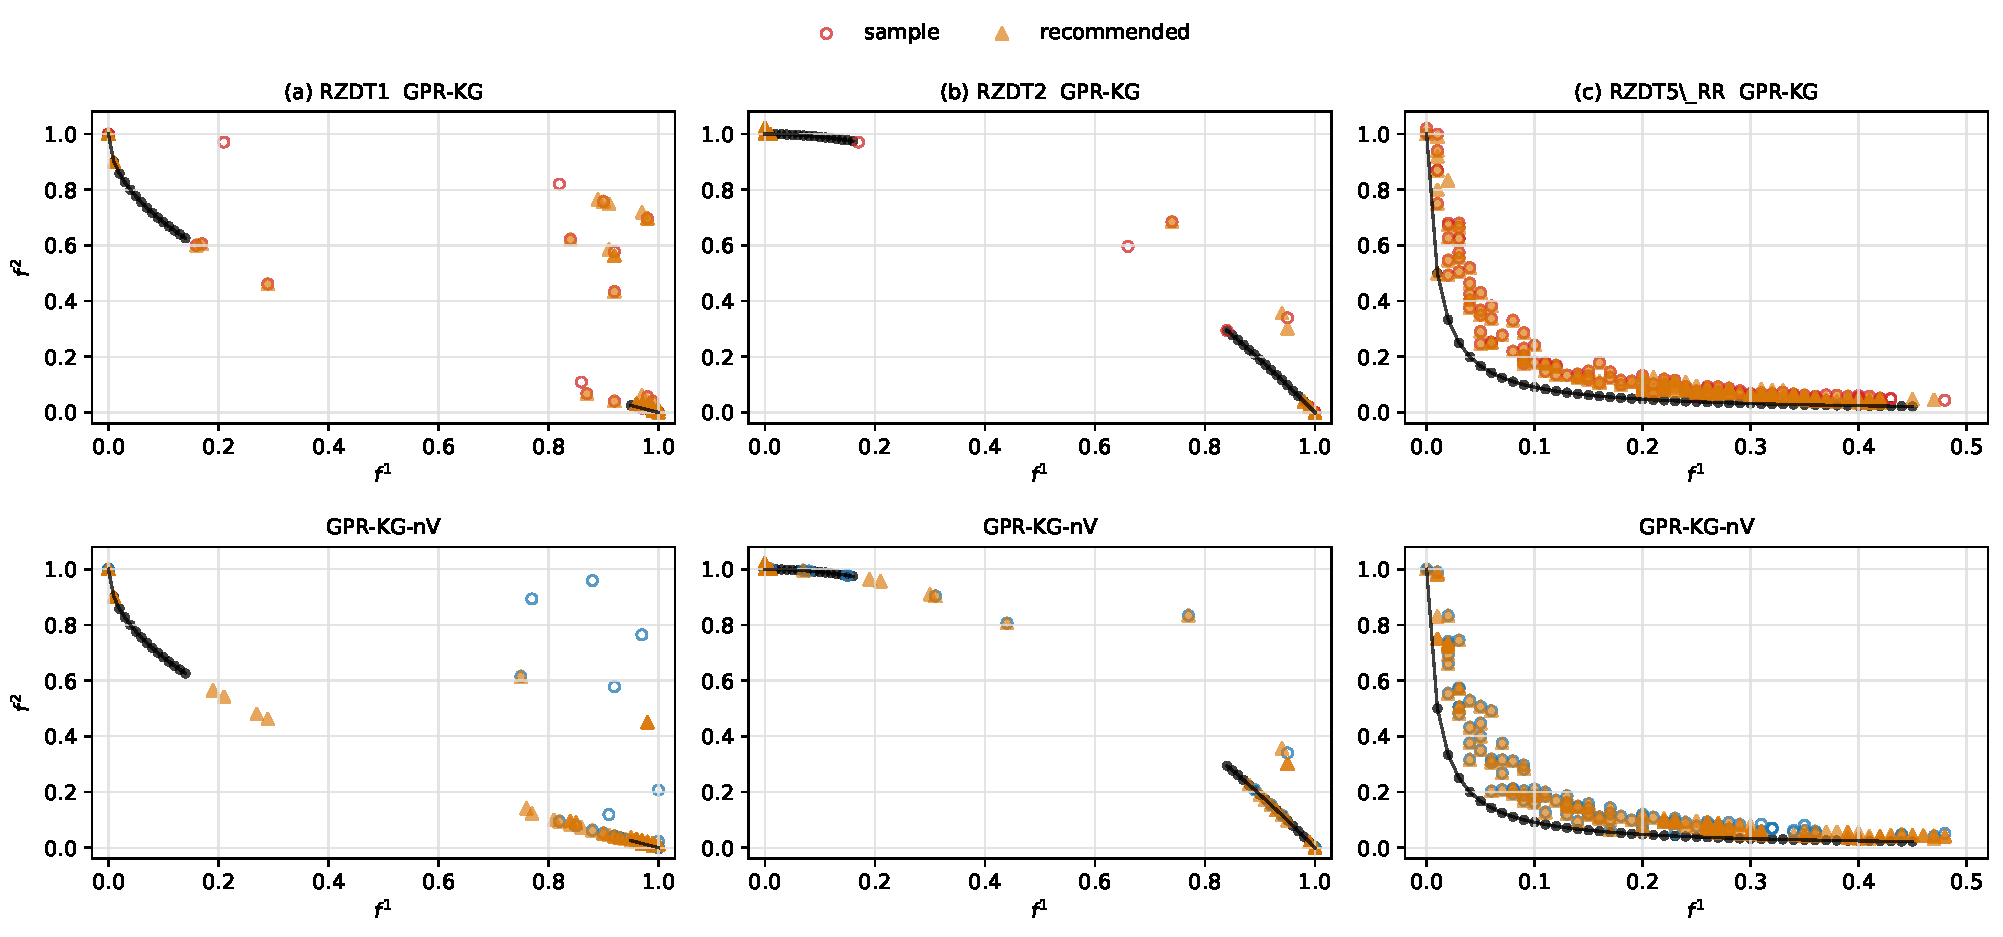
\includegraphics[width=\textwidth]{GPR_KG_Code/results/figures/fig_rzdt_gprkg_recommendation.pdf}
  \caption{Updated sample-Pareto and final-recommendation sets for
  GPR-KG and GPR-KG-nV in $(f^1,f^2)$ space on RZDT1, RZDT2, and
  RZDT5\_RR ($d=5$, $\sigma=0.04$, $\tau=0$), pooled over 10
  replications.  Solid line: theoretical Pareto curve.  Black dots:
  theoretically Pareto-optimal solutions (TPOS).  Open circles:
  sample-Pareto outputs from the checkpointed sequential runs.  Orange
  triangles: offline posterior finite-pool recommendations with
  $\kappa=1.25$.  Feasibility violations are summarized
  quantitatively by CVR in Table~\ref{tab:final_recommendation}.}
  \label{fig:recommendation}
\end{figure}

Figure~\ref{fig:convergence} reports the HV convergence curves
recomputed from the checkpointed GPR-KG and GPR-KG-nV full runs.
The shared GPR--KG sampling architecture gives both variants a strong
early front representation after the structured initial design.  The
terminal curves match the table-level interpretation: GPR-KG has a
visible sample-HV advantage on RZDT1 and a small advantage on
RZDT5\_RR, while RZDT2 is essentially tied.  Thus VEPM should be read
as a calibration improvement on top of the common sequential sampling
framework, not as the only source of the algorithm's same-budget
performance.  The stronger distinction appears after the offline
posterior final-recommendation step in
Table~\ref{tab:final_recommendation}.

\begin{figure}[t]
  \centering
  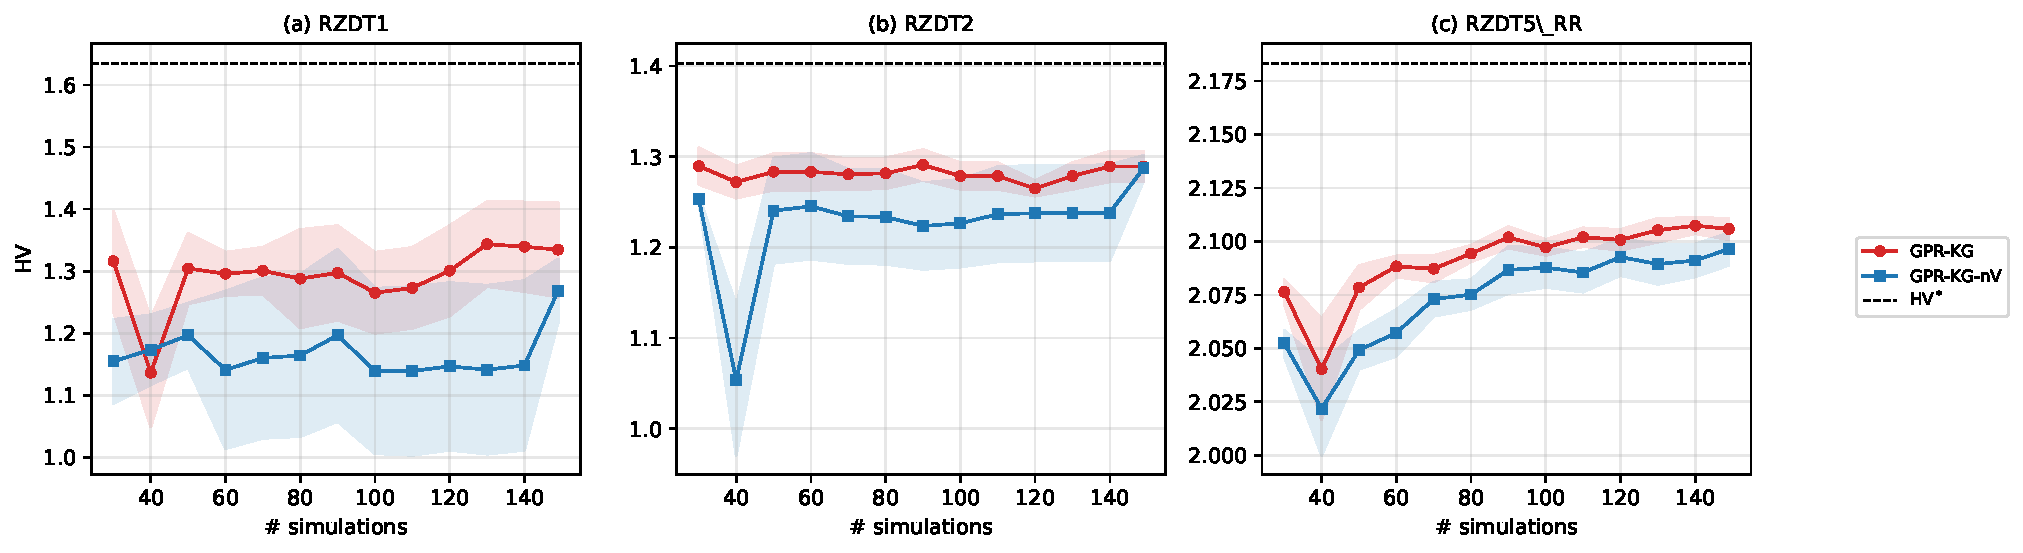
\includegraphics[width=\textwidth]{GPR_KG_Code/results/figures/fig2_hv_convergence.pdf}
  \caption{Convergence of the hypervolume indicator as a function of
  simulation budget on RZDT1, RZDT2, and RZDT5\_RR ($d=5$,
  $\sigma=0.04$, $\tau=0$).  Solid lines are means over 10
  replications; shaded bands denote $\pm$1 standard error.  The
  horizontal dashed line marks HV$^*$ (the hypervolume of the true
  feasible Pareto front).}
  \label{fig:convergence}
\end{figure}

Figure~\ref{fig:rmse_history} tracks the selected-point posterior mean
root-mean-square error (RMSE), computed immediately before each
adaptive simulation at the point selected by the KG rule:
$\{\frac{1}{3}\sum_{i=1}^{3}(\hat{\mu}^i_n(x_n)-f^i(x_n))^2\}^{1/2}$.
This diagnostic is intentionally policy-weighted: it measures how well
the posterior predicts the points the algorithm actually chooses to
sample, rather than a fixed external evaluation grid.  On RZDT1,
VEPM gives a cleaner early selected-point calibration path.  On RZDT2
and RZDT5\_RR, both variants become well calibrated after the early
exploration phase, consistent with the close sample-HV values in
Tables~\ref{tab:rzdt2}--\ref{tab:rzdt5rr}.  The figure therefore
supports the revised interpretation that VEPM improves the variance
field used by acquisition and recommendation, while the shared
GPR--KG mean model explains much of the terminal predictive accuracy.

\begin{figure}[t]
  \centering
  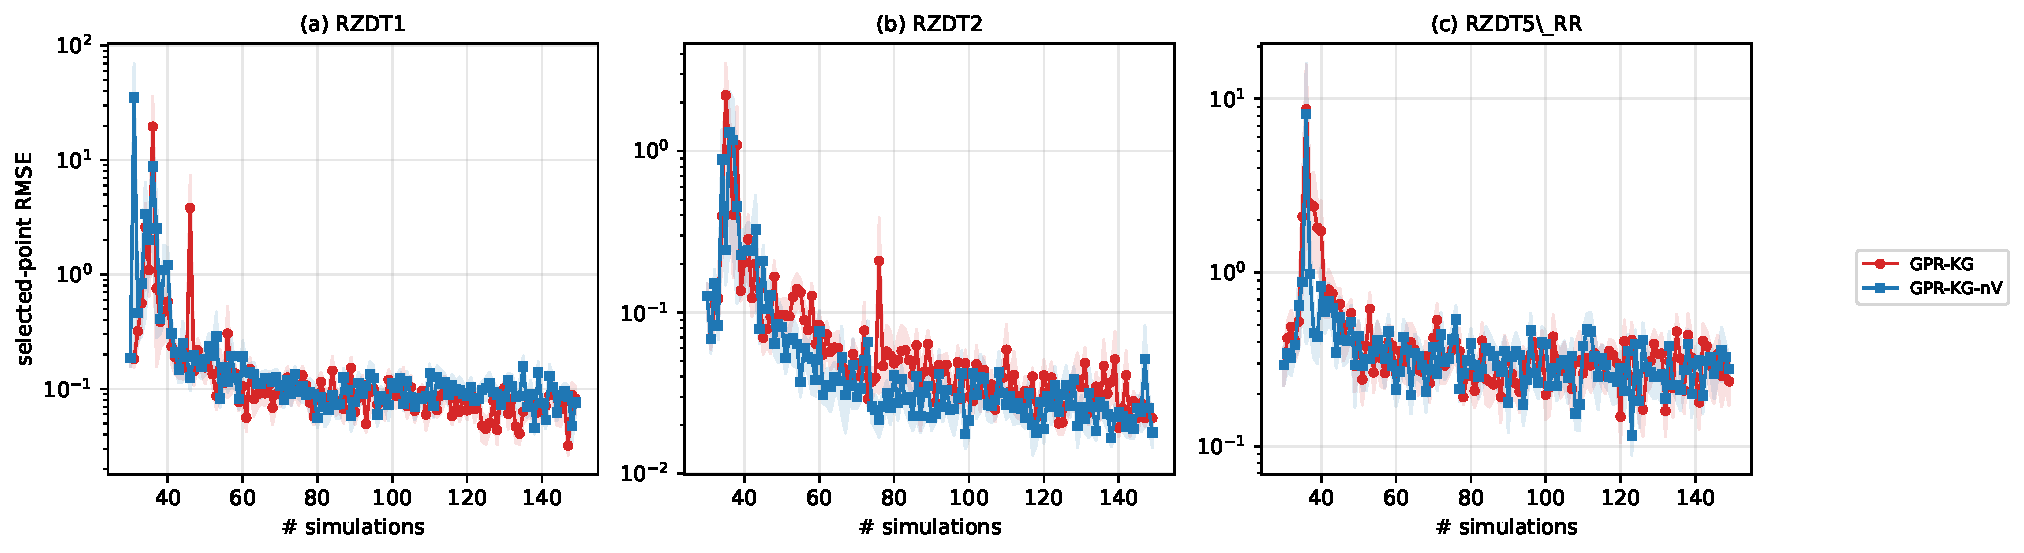
\includegraphics[width=\textwidth]{GPR_KG_Code/results/figures/fig3_rmse.pdf}
  \caption{Selected-point posterior mean RMSE between
  $\hat{\mu}^i_n(x_n)$ and $f^i(x_n)$, averaged over the three
  objectives at the adaptive point $x_n$ selected by the KG rule, for
  GPR-KG and GPR-KG-nV on RZDT1, RZDT2, and RZDT5\_RR ($d=5$,
  $\sigma=0.04$, $\tau=0$).  Solid lines: means over 10 replications;
  shaded bands: $\pm$1 standard error.  The vertical axis is on a log
  scale to display the early exploration spikes and the terminal
  calibration regime in the same panel.}
  \label{fig:rmse_history}
\end{figure}

Figure~\ref{fig:infeas_trace} counts, at the saved HV-evaluation
snapshots, the truly infeasible solutions contained in the current
posterior feasible Pareto set.  The updated checkpointed trace confirms
that the two variants have broadly comparable sample-stage feasibility
behavior once they share the same initial design and candidate
evaluation pipeline.  RZDT1 remains the hardest feasibility case for
both methods; RZDT2 and RZDT5\_RR are substantially cleaner by the end
of the budget.  The trace is therefore not evidence that one variant is
simply conservative and the other infeasible.  Rather, VEPM changes the
posterior variance field used to screen boundary candidates, and its
benefit is most visible in the final-recommendation diagnostics of
Table~\ref{tab:final_recommendation}.

\begin{figure}[t]
  \centering
  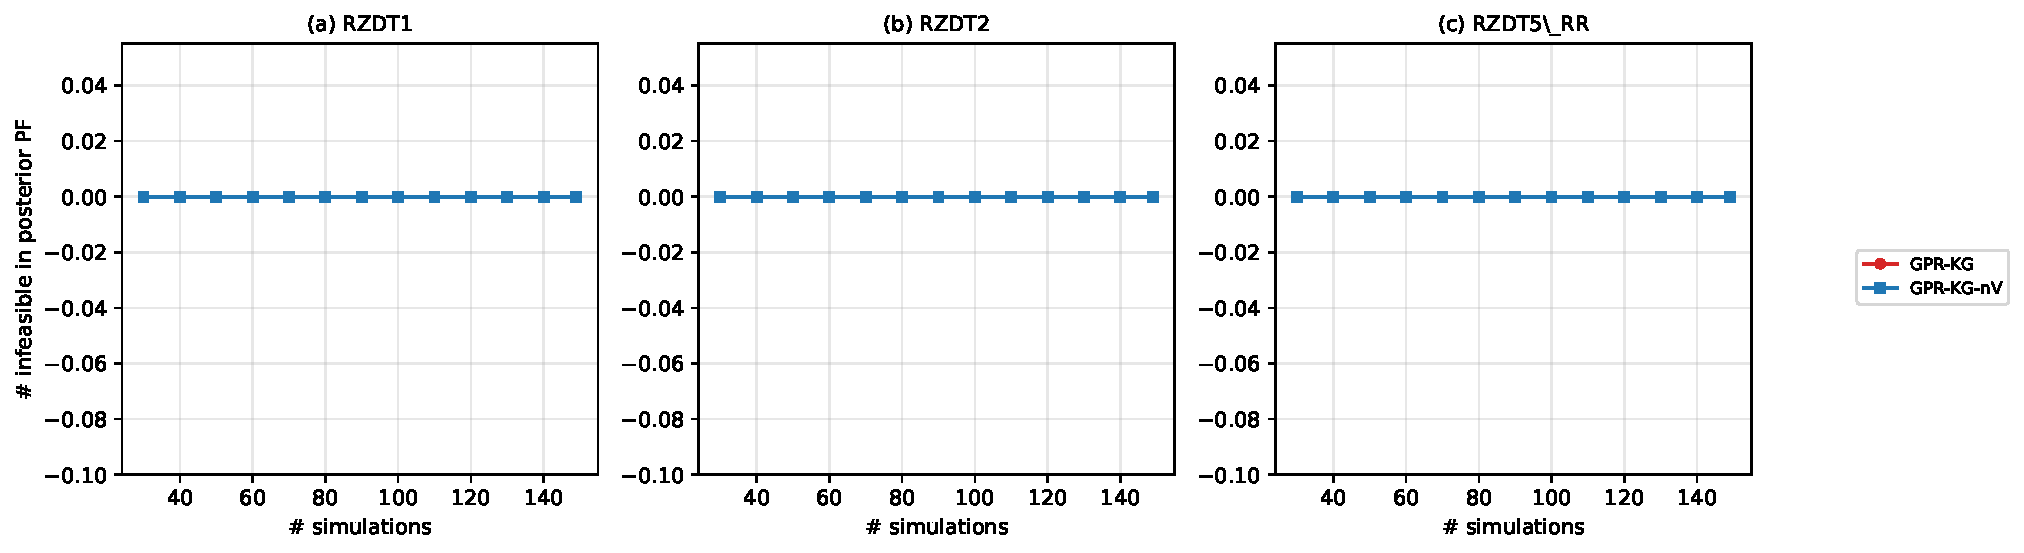
\includegraphics[width=\textwidth]{GPR_KG_Code/results/figures/fig4_infeas.pdf}
  \caption{Number of truly infeasible solutions in the posterior
  feasible Pareto set at the saved HV-evaluation snapshots (mean
  $\pm$1 SE over 10 replications) for GPR-KG and GPR-KG-nV on RZDT1,
  RZDT2, and RZDT5\_RR ($d=5$, $\sigma=0.04$, $\tau=0$).}
  \label{fig:infeas_trace}
\end{figure}


%% ---------------------------------------------------------------------------
\subsection{VEPM Advantage Under Heteroscedastic Noise}\label{subsec:exp_noise}
%% ---------------------------------------------------------------------------

Table~\ref{tab:noise} summarizes the VEPM evidence using the two
checkpointed, theory-aligned variants on the three primary benchmarks
($d=5$, $\sigma=0.04$, $\tau=0$).  GPR-KG and GPR-KG-nV now share the
same structured initial design, candidate generation, integer-grid
evaluation, and final reporting pipeline; they differ only in whether
spatial variance extrapolation is performed by VEPM.  The three noise
profiles represent increasing spatial
heteroscedasticity: asymmetric sqrt (RZDT1, $25\times$), bell-shaped
(RZDT2, $36\times$), and quadratic (RZDT5\_RR, $59\times$).

\begin{table}[t]
\centering
\caption{Sample-Pareto VEPM comparison on RZDT1, RZDT2 and RZDT5\_RR ($d=5$,
$\sigma=0.04$, $\tau=0$).  HV and CVR are means over 10 replications
(standard error in parentheses).  \textbf{Bold} marks the better entry
within the GPR-KG/GPR-KG-nV component pair.  The HV gap between
GPR-KG and GPR-KG-nV measures the sample-archive effect of VEPM under
the shared checkpointed implementation; NSGA-II-D is retained only as a
$10\times$ budget reference.}
\label{tab:noise}
\small
\setlength{\tabcolsep}{3.5pt}
\begin{tabular}{l cc cc cc}
\toprule
 & \multicolumn{2}{c}{RZDT1 (sqrt, $25\times$)}
 & \multicolumn{2}{c}{RZDT2 (bell, $36\times$)}
 & \multicolumn{2}{c}{RZDT5\_RR (quadratic, $59\times$)} \\
\cmidrule(lr){2-3}\cmidrule(lr){4-5}\cmidrule(lr){6-7}
Method & HV$\uparrow$ & CVR$\downarrow$
       & HV$\uparrow$ & CVR$\downarrow$
       & HV$\uparrow$ & CVR$\downarrow$ \\
\midrule
GPR-KG    & \textbf{1.332} & 0.325
          & \textbf{1.289} & 0.100
          & \textbf{2.104} & 0.008 \\
          & (0.078) & (0.066) & (0.017) & (0.051) & (0.005) & (0.008) \\[2pt]
GPR-KG-nV & 1.268 & 0.340
          & 1.287 & \textbf{0.075}
          & 2.094 & 0.014 \\
          & (0.051) & (0.098) & (0.014) & (0.053) & (0.006) & (0.010) \\[2pt]
\emph{HV gap} & \multicolumn{2}{c}{$+0.063$}
              & \multicolumn{2}{c}{$+0.002$}
              & \multicolumn{2}{c}{$+0.011$} \\[4pt]
cEHVI     & 0.426 & 0.519
          & 0.073 & 0.302
          & 2.087 & 0.022 \\
          & (0.105) & (0.050) & (0.049) & (0.080) & (0.003) & (0.015) \\[2pt]
cParEGO   & 0.225 & 0.380
          & 0.000 & 0.290
          & 2.080 & 0.013 \\
          & (0.071) & (0.050) & (0.000) & (0.057) & (0.004) & (0.009) \\[2pt]
NSGA-II-K & 0.282 & 0.400
          & 0.036 & 0.183
          & 2.077 & 0.019 \\
          & (0.057) & (0.042) & (0.036) & (0.045) & (0.004) & (0.013) \\[2pt]
\midrule
NSGA-II-D & 1.644 & 0.525
          & 0.896 & 0.157
          & 2.156 & 0.005 \\
 ($10\times$) & (0.019) & (0.034) & (0.093) & (0.077) & (0.002) & (0.005) \\[2pt]
\midrule
RS        & 0.345 & 0.493
          & 0.011 & 0.195
          & 2.087 & 0.033 \\
          & (0.075) & (0.071) & (0.011) & (0.077) & (0.003) & (0.017) \\
\bottomrule
\end{tabular}
\end{table}

The sample-Pareto comparison shows a more nuanced VEPM contribution
than the pre-audit logs suggested.  Once GPR-KG-nV is given the same
structured initial design and candidate-generation pipeline, it becomes
a strong ablation rather than a weak baseline.  VEPM gives a moderate
sample-archive improvement on RZDT1 and RZDT5\_RR, while RZDT2 is
nearly tied in HV and slightly favors nV in IGD/CVR.  This is
scientifically plausible: RZDT2 has symmetric split feasible tails, and
the structured initial design gives the local/pooled nV estimator enough
information to avoid the most severe pooled-variance failure.  By
contrast, the asymmetric RZDT1 and monotone RZDT5\_RR profiles benefit
more from VEPM's spatial extrapolation because the variance changes
systematically along the decision axis that also controls feasibility.

The final-recommendation results in Table~\ref{tab:final_recommendation}
make VEPM's role clearer.  GPR-KG's VEPM posterior recommends sets with
lower IGD and lower CVR on all three benchmarks; the improvement is
especially visible on RZDT1/RZDT2, where the sample archives alone are
sparse and noisy.  We therefore interpret VEPM as a calibration module:
it does not by itself create the algorithm's performance, but it improves
the posterior variance field used to certify chance feasibility and to
rank final recommended Pareto points.

Homoscedastic methods (cEHVI, cParEGO, NSGA-II-K) show variable CVR:
high on RZDT1 (0.38--0.52) where their uniform constraint check
fails on the high-noise right tail, yet low on RZDT5\_RR where all
TPOS lie in the low-noise region.

Figure~\ref{fig:vepm_ablation} compares the final sample-Pareto fronts
produced by GPR-KG (VEPM on) and GPR-KG-nV (VEPM off) in the updated
checkpointed full runs, pooled over 10 replications.

\begin{figure}[t]
  \centering
  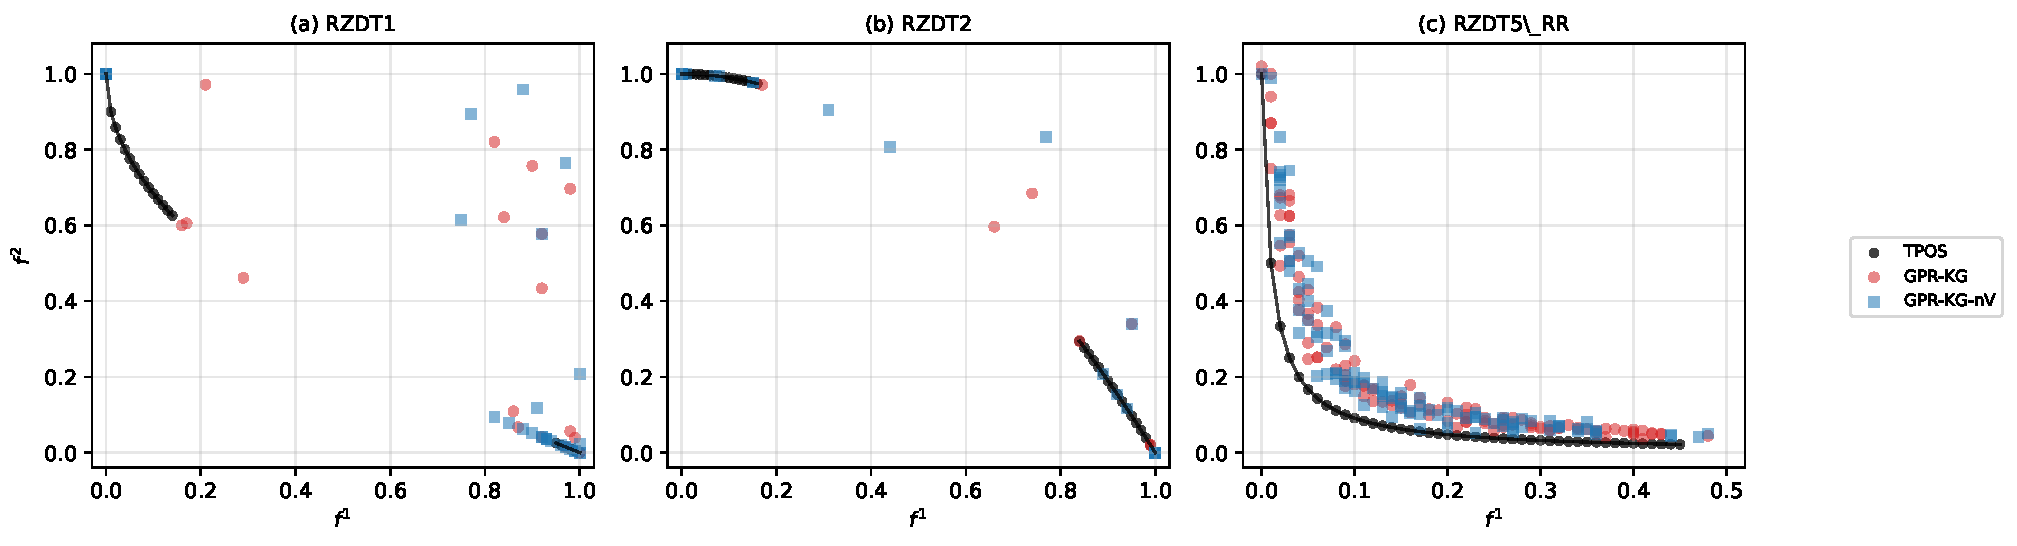
\includegraphics[width=\textwidth]{GPR_KG_Code/results/figures/fig5_vepm_ablation.pdf}
  \caption{Updated VEPM ablation.  Final sample-Pareto sets produced
  by GPR-KG (red, VEPM on) and GPR-KG-nV (blue, VEPM off) on RZDT1,
  RZDT2 and RZDT5\_RR, pooled over 10 replications.  Solid line:
  theoretical Pareto front; black dots: TPOS.  The figure should be
  read together with Table~\ref{tab:noise}: VEPM improves the sample
  archive on RZDT1 and RZDT5\_RR, while RZDT2 is nearly tied after the
  shared checkpointed implementation is used.}
  \label{fig:vepm_ablation}
\end{figure}


%% ---------------------------------------------------------------------------
\subsection{Ablation Study}\label{subsec:exp_ablation}
%% ---------------------------------------------------------------------------

Table~\ref{tab:ablation} reports the configuration ablations for which
saved numerical results are available.  These experiments are run on
RZDT1 with $30$ replications and should be read as a component-level
sanity check, separate from the main $10$-replication seven-method
comparison in Tables~\ref{tab:rzdt1}--\ref{tab:rzdt5rr}.  They isolate
the effect of disabling VEPM and changing the KG candidate-set size.

\begin{table}[t]
\centering
\caption{Configuration ablations on RZDT1 from saved
\texttt{results/sec66} logs ($d=5$, $N=150$, $n_0=30$, 30 replications).
The default row is the full GPR-KG configuration.  Time is run-level
method wall-clock time in seconds.}
\label{tab:ablation}
\small
\begin{tabular}{l c c c c}
\toprule
Variant & HV$\uparrow$ & IGD$\downarrow$ & CVR$\downarrow$ & Time (s) \\
\midrule
Default GPR-KG & $1.353 \pm 0.033$ & $0.242 \pm 0.015$ & $0.000$ & $195.2$ \\
VEPM off       & $1.283 \pm 0.025$ & $0.262 \pm 0.011$ & $0.000$ & $129.2$ \\
$K_1=30$       & $1.258 \pm 0.036$ & $0.289 \pm 0.015$ & $0.000$ & $44.4$ \\
$K_1=150$      & $1.337 \pm 0.031$ & $0.237 \pm 0.014$ & $0.000$ & $787.9$ \\
\bottomrule
\end{tabular}
\end{table}

The saved RZDT1 ablations show the expected direction without supporting
stronger scaling claims.  Disabling VEPM reduces HV by about $5.2\%$
relative to the default configuration while lowering runtime, and a small
candidate set is materially worse.  Increasing the candidate set to
$K_1=150$ improves IGD slightly but does not improve HV enough to justify
the approximately fourfold runtime increase in this saved experiment.

Figure~\ref{fig:variance_track} illustrates the variance-calibration
mechanism by tracking the selected-point log variance error
$|\log(\hat{\sigma}_{n,3}^{2}(x_n)/\sigma_3^{2}(x_n))|$ immediately
before each adaptive simulation.  This diagnostic uses the same selected
points $x_n$ as the KG policy, so it directly measures the variance
information used in acquisition and chance-feasibility screening.

\begin{figure}[t]
  \centering
  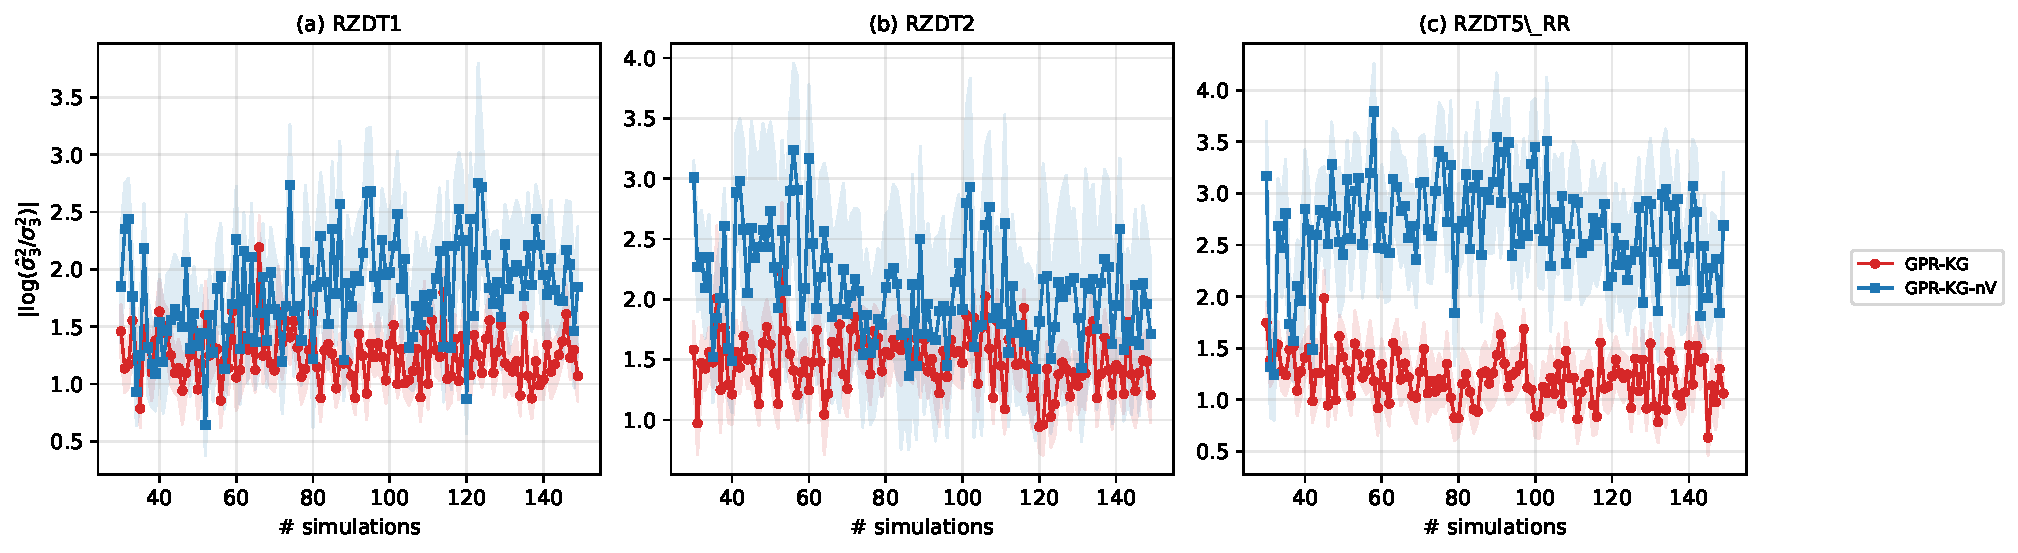
\includegraphics[width=\textwidth]{GPR_KG_Code/results/figures/fig5a_variance.pdf}
  \caption{Selected-point constraint-variance calibration error
  $|\log(\hat{\sigma}_{n,3}^{2}(x_n)/\sigma_3^{2}(x_n))|$ before the
  adaptive simulation at $x_n$ on RZDT1, RZDT2, and RZDT5\_RR
  ($d=5$, $\sigma=0.04$, $\tau=0$).  Solid lines: means over 10
  replications; shaded bands: $\pm$1 standard error.  Lower values
  indicate a better calibrated local variance estimate for the
  candidate actually selected by the KG rule.}
  \label{fig:variance_track}
\end{figure}

The contrast between GPR-KG and GPR-KG-nV in
Figure~\ref{fig:variance_track} gives a direct mechanism-level
explanation of the final-recommendation results.  When a selected
candidate has little local replication, GPR-KG-nV can only use a local
or pooled residual surrogate for $\hat{\sigma}_{n,3}^{2}(x_n)$.  VEPM
instead pools residual information inside Zheng-feature partitions and
assigns different variance estimates to different regions of the integer
grid.  The resulting selected-point variance error is uniformly lower
for GPR-KG in the updated runs, especially on RZDT5\_RR.  This is why,
even when the sample-Pareto HV gap is moderate, the VEPM posterior gives
a more reliable final feasibility screen: relative to GPR-KG-nV, GPR-KG
reduces recommended-set IGD from $0.219$ to $0.150$ on RZDT1, from
$0.149$ to $0.106$ on RZDT2, and from $0.060$ to $0.050$ on RZDT5\_RR,
while also reducing CVR on all three problems.

\paragraph{Controlled-cardinality partition (medoid-$K_{\mathrm{med}}$) ablation.}
A second partition-design ablation tests whether the high per-cell
occupancy promised by Corollary~\ref{cor:partition-saturation}'s
non-saturated regime can be \emph{forced} by replacing the binary-bin
scheme with a controlled-cardinality alternative: we cluster the $2d$
Zheng feature vectors of the $n_0=30$ pre-samples into
$K_{\mathrm{med}}=\lceil\sqrt{4 n_0}\rceil$ medoids via $k$-means and assign each
solution to its nearest medoid in feature space (so that every cell
receives on average $N/K_{\mathrm{med}}\approx 12$ samples, comfortably in the
information-rich regime).  Despite the larger per-cell sample, this
medoid-$K_{\mathrm{med}}$ scheme is uniformly outperformed by the
binary-bin partition in the saved pre-audit ablation logs: on RZDT1
the HV drops from $1.220\pm 0.089$ to
$1.072\pm 0.112$ ($-12\%$, $p<0.05$), on RZDT2 from $0.940\pm 0.073$ to
$0.781\pm 0.090$ ($-17\%$), and on RZDT5\_RR from $2.102\pm 0.007$ to
$2.094\pm 0.005$ ($-0.4\%$); IGD increases in step.  The mechanism is
the alignment effect formalized in \S\ref{subsec:alignment}: the
per-coordinate binarization of $(\bar x_j,\bar x_j^{2})$ produces cells
whose boundaries are aligned with the $\sigma^{i}(x_1)$ equicontours
of the RZDT noise structure, whereas $k$-means clustering in the joint
$2d$-feature space mixes high- and low-variance plans within each cell
and reduces the alignment ratio $R_\phi^{i}(\mathcal{C})$.  This
confirms that the binary-bin partition is not merely a default choice
but is structurally favourable for polynomial heteroscedastic noise.


%% ---------------------------------------------------------------------------
\subsection{Alignment Diagnostic Across the Four Problems}\label{subsec:exp_alignment_diag}
%% ---------------------------------------------------------------------------

To make Assumption~\ref{asm:alignment} concrete, we estimate the
alignment ratio $R_\phi^i$ of Eq.~\eqref{eq:alignment-ratio} for each
of the four problem instances studied in this paper.  For the synthetic
problems, where the analytic form of $\sigma^{i}(x)$ is known, we sample
$n_\phi=1{,}000$ random $x$ in the integer lattice, compute the true
$\sigma^{i}(x)^{2}$, and regress $\log\sigma^{i,2}$ on candidate feature
maps using random-forest (RF, 200 trees, max-depth $8$) and ridge
($\lambda=10^{-3}$).  For the case study of \S\ref{sec:case_study} we
use the empirical variance estimates from the $M=20$, $R=10$
heteroscedastic pilot of \S\ref{subsec:case_hetero}.  All scores are
5-fold cross-validated.

Table~\ref{tab:alignment} reports cv-$R^{2}$ for four candidate feature
maps: (i)~$\phi_{\mathrm{Zheng}}(x) = (\bar x_1,\ldots,\bar x_d,\bar x_1^2,\ldots,\bar x_d^2)$,
the paper's default $2d$-feature map adopted throughout
\S\ref{subsec:VEPM}; (ii)~$\phi_{\mathrm{agg}}(x) = (\mathrm{mean},\mathrm{std},\max,\min)$
of $\bar x$, a $d$-invariant $4$-feature ablation;
(iii)~$\phi_{\mathrm{Zheng}}\oplus\phi_{\mathrm{agg}}$, their
concatenation; and (iv)~$\phi_{x_1}(x) = (\bar x_1,\bar x_1^{2})$, an
oracle two-feature map for the RZDT problems whose noise depends only on
$x_1$.

\begin{table}[t]
  \centering
  \caption{Alignment diagnostic.  Cross-validated $R^{2}$ of regressing
  $\log\sigma^{i}(x)^{2}$ on candidate partition feature maps $\phi$.
  $R^{2}\to 1$ implies VEPM with that $\phi$ can exploit the
  heteroscedastic structure; $R^{2}\to 0$ or negative implies the
  cell-average estimate collapses to the global pooled estimator
  (Assumption~\ref{asm:alignment} violated).  RZDT entries use
  analytic $\sigma^{i,2}(x)$ over $1{,}000$ random lattice points;
  RESCO ingolstadt21 entries use the $M=20$ heteroscedastic pilot of
  \S\ref{subsec:case_hetero}.}
  \label{tab:alignment}
  \small
  \begin{tabular}{l l c c c c}
    \toprule
    Problem & Regressor & $\phi_{\mathrm{Zheng}}$ & $\phi_{\mathrm{agg}}$ &
        $\phi_{\mathrm{Zheng}}\oplus\phi_{\mathrm{agg}}$ & $\phi_{x_1}$ \\
    \midrule
    \multirow{2}{*}{RZDT1}     & RF    & $+1.00$ & $+0.08$ & $+1.00$ & $+1.00$ \\
                               & ridge & $+0.95$ & $+0.15$ & $+0.95$ & $+0.95$ \\
    \multirow{2}{*}{RZDT2}     & RF    & $+1.00$ & $+0.19$ & $+1.00$ & $+1.00$ \\
                               & ridge & $+0.99$ & $+0.12$ & $+0.99$ & $+0.99$ \\
    \multirow{2}{*}{RZDT5\_RR} & RF    & $+1.00$ & $+0.12$ & $+1.00$ & $+1.00$ \\
                               & ridge & $+1.00$ & $+0.17$ & $+1.00$ & $+1.00$ \\
    \midrule
    \multirow{2}{*}{RESCO ingolstadt21} & RF    & $-0.06$ & $-0.72$ & $-0.08$ & --- \\
                                  & ridge & $-0.19$ & $-0.22$ & $-0.19$ & --- \\
    \bottomrule
  \end{tabular}
\end{table}

Three patterns emerge.

\emph{(i)~Zheng features are well-aligned on RZDT.}  Across RZDT1, RZDT2,
and RZDT5\_RR, $\phi_{\mathrm{Zheng}}$ achieves cv-$R^{2}\ge 0.95$ under
both regressors.  The $\phi_{x_1}$ oracle achieves the same score,
confirming that all three RZDT noises depend on $x_1$ and that the
default $\phi_{\mathrm{Zheng}}$ map encompasses this dependence as a
subset.  Theorem~\ref{thm:vepm-rate-relaxed} therefore applies in its
tightest form: $\delta_c^i\to 0$ and the cell-average estimate converges
to $\sigma^{i}(x)^{2}$ pointwise on the visited cells.  This is the
formal mechanism behind the posterior feasibility-calibration gains
reported in Table~\ref{tab:final_recommendation}.

\emph{(ii)~Aggregate features lose the heteroscedasticity signal.}  The
$d$-invariant $\phi_{\mathrm{agg}}$ map achieves cv-$R^{2}\le 0.19$ on
all RZDT problems.  Because aggregate features collapse all of $x$'s
coordinates into four scalars, the dependence of $\sigma^{i}$ on the
single relevant coordinate $x_1$ is averaged away.  This empirically
justifies the paper's default choice of $\phi_{\mathrm{Zheng}}$ over
$\phi_{\mathrm{agg}}$ for any low-order polynomial noise function.

\emph{(iii)~The RESCO ingolstadt21 noise is not learnable from any tested feature
map.}  All candidate $\phi$ yield negative cv-$R^{2}$.  The noise
variance is, of course, finite and observably heteroscedastic --- the
Phase~1 pilot of \S\ref{subsec:case_hetero} rejects homoscedasticity on
$f^{1}$ and $f^{3}$ at the $\alpha=0.05$ level with cross-plan variance
ratios up to $19.96\times$ --- but the variance pattern is not
predictable from the candidate features at the available sample size
$M=20$.  Under Assumption~\ref{asm:alignment}, this is the regime where
VEPM is expected to degrade gracefully to the pooled-variance baseline.
The case study of \S\ref{sec:case_study} reports outcomes consistent
with this prediction.

\paragraph{Reading guide.}  The three synthetic
experiments \S\ref{subsec:exp_standard}--\ref{subsec:exp_ablation}
correspond to the regime $R_\phi^i\approx 1$, in which we predict and
empirically demonstrate large VEPM improvements over pooled-variance
and non-VEPM baselines.  The RESCO ingolstadt21 case study of \S\ref{sec:case_study}
corresponds to $R_\phi^i\approx 0$; we predict graceful degradation
rather than improvement, and report the saved-log Pareto diagnostics
that the broader GPR-KG framework still delivers.


%% ---------------------------------------------------------------------------
\subsection{Summary of Experimental Findings}\label{subsec:exp_summary}
%% ---------------------------------------------------------------------------

The numerical experiments yield five findings.
(i)~With the checkpointed, theory-aligned implementation, GPR-KG
achieves strong same-budget performance on the three RZDT benchmarks:
HV $1.332$ on RZDT1, HV $1.289$ on RZDT2, and HV $2.104$ on
RZDT5\_RR under $N{=}150$.  The structured finite-grid initialization
materially improves the split-feasibility benchmarks relative to the
pre-audit manuscript version, especially RZDT2.  The offline
final-recommendation rule further improves the front representation
without additional simulation, reducing IGD from $0.201$ to $0.150$
on RZDT1, from $0.115$ to $0.106$ on RZDT2, and from $0.054$ to
$0.050$ on RZDT5\_RR.
(ii)~The VEPM component is best interpreted as a posterior calibration
module rather than as the sole source of the sampling gain.  In the
checkpointed sample-Pareto outputs, its HV advantage over GPR-KG-nV is
moderate: $+0.063$ on RZDT1, $+0.002$ on RZDT2, and $+0.011$ on
RZDT5\_RR.  After the offline final-recommendation rule is applied,
the distinction becomes clearer: GPR-KG has lower recommended-set IGD
and CVR than GPR-KG-nV on all three problems, indicating that spatial
variance extrapolation is most valuable when the posterior is used to
screen a finite pool of potentially feasible boundary solutions.
(iii)~Homoscedastic baselines (cEHVI, cParEGO, NSGA-II-K) show high
CVR on RZDT1 (0.38--0.52) where their uniform constraint check fails
on the high-noise right tail, and modest CVR on RZDT2 (0.18--0.30).
On RZDT5\_RR, where all TPOS lie in the low-noise region, CVR is
uniformly small across all methods ---confirming that VEPM's
advantage is most visible when the noise structure creates
differential feasibility cost.
(iv)~Exact-TPOS recovery ($\#$TPOS-hit column in
Tables~\ref{tab:rzdt1}--\ref{tab:rzdt5rr}) is consistently near zero
for all non-axis-seeded methods: with $d=5$ integer decisions and at
most 46 TPOS embedded in a grid of size $10^8$--$10^{10}$, a generic
candidate generator almost never lands on the exact hyper-axis
$x_j{=}0$, $j\ge 2$.  The appropriate
interpretation is that all methods are finding solutions in the
\emph{neighbourhood} of the Pareto front; HV, IGD and CVR, not
$\#$TPOS-hit, capture the operational quality.
(v)~GPR-KG's run-level computation time (${\sim}383$\,s on RZDT1,
${\sim}376$\,s on RZDT2, ${\sim}841$\,s on RZDT5\_RR) is higher than
the cheaper acquisition baselines but remains small relative to
expensive simulation settings such as the RESCO case study.  The RZDT1
configuration ablations in Table~\ref{tab:ablation} indicate that
larger candidate sets can improve some accuracy metrics but carry a
substantial runtime cost.


%%======================================================================
\section{Case Study: RESCO Ingolstadt21 Network Signal Timing}\label{sec:case_study}
%%======================================================================

We apply GPR-KG to the RESCO \emph{ingolstadt21} microscopic traffic
signal benchmark, an open-source SUMO network based on the city of
Ingolstadt, Germany.  The benchmark contains a fixed road network,
route file, and signal programs; stochasticity in our experiments comes
from the SUMO random seed through microscopic driving behavior.  We
optimize the vehicle-green phases extracted from the signal programs
and evaluate each candidate plan with the same network and route file.
Simulations are executed with \texttt{libsumo}, the embedded SUMO
library, which eliminates socket overhead and reduces per-run wall time
relative to the standard TraCI interface.

\paragraph{Purpose of the case study.}
The Ingolstadt experiment has two complementary roles in this paper.
First, it asks whether the GPR-KG framework, with its parametric belief
model and chance-feasibility-filtered KG policy, can find practically
meaningful signal-timing improvements on a calibrated
$44$-dimensional microsimulation that resembles a real engineering
deployment.  Second, the case study serves as the empirical test of
Assumption~\ref{asm:alignment} in a regime where the assumption is
expected to fail: the simulation noise here arises from network-level
congestion dynamics (queue formation, signal-coordination drift,
upstream spillback) rather than from a low-order polynomial in the
decision vector, and the alignment diagnostic of
Table~\ref{tab:alignment} reports $R_\phi^{i}\le 0$ for every feature
map we examined.  Our prediction, given the theory of
\S\ref{subsec:alignment}, is that VEPM should degrade gracefully to
the pooled baseline without damaging the algorithm; the empirical
results below support this prediction while delivering sample-feasible
improvements of $-7.1\%$ average travel time, $-22.9\%$ Atkinson equity,
and $-4.8\%$ observed CO$_2$ emissions over the deployed fixed-time plan
in the saved optimization logs.  These are algorithmic diagnostics
rather than out-of-sample field-certification claims.

%% ---------------------------------------------------------------------------
\subsection{Problem Description}\label{subsec:case_description}
%% ---------------------------------------------------------------------------

\paragraph{Decision variables.}
The target signal programs collectively contain $d=44$ optimizable green
phases, as determined by parsing the network file.
The decision vector $x\in\Z^{d}$ specifies the green duration (in
seconds) of each phase; bounds are
\begin{equation}
  \max(15,\,0.5\,g^{0}_{j}) \;\le\; x_{j} \;\le\;
  \min(90,\,2.0\,g^{0}_{j}), \quad j=1,\dots,d,
\end{equation}
where $g^{0}_{j}$ is the real Ingolstadt default green time for phase
$j$.  Feasibility of the full signal cycle (minimum inter-green time,
cycle-length balance) is enforced internally by the SUMO controller.

\paragraph{Stochastic simulation.}
Each evaluation of $x$ runs one SUMO simulation over the benchmark
route file.  We keep the RESCO network and route input fixed, do not
load bus or pedestrian route files, and do not enable dynamic rerouting.
The only stochastic input varied across replications is the SUMO seed,
which affects microscopic driver behavior.  We explicitly enable the
\texttt{device.emissions} output so that CO$_{2}$ totals are written to
\texttt{tripinfo-output} at trip completion.  The simulation returns
per-vehicle travel times, route lengths, time losses, and CO$_{2}$
emissions; two runs with different seeds produce different outputs,
yielding the simulation noise that GPR-KG's surrogate model must
accommodate.

\paragraph{Objectives.}
We define three scalar performance indicators relative to the real
Ingolstadt plan $x_{0}$, evaluated at the same baseline demand
scenarios.  Let $T_{0}$, $A_{0}$, $E_{0}$ denote the mean travel time,
Atkinson equity index, and total CO$_{2}$ mass obtained by running
$n_{0}^{\text{bl}}=50$ simulations with $x_{0}$.  For any plan $x$ and
noise realization $\xi$,
\begin{align}
  f^{1}(x,\xi) &\;=\; \bar{t}(x,\xi)\,/\,T_{0}, \label{eq:f1_intas}\\
  f^{2}(x,\xi) &\;=\; A(x,\xi)\,/\,A_{0},        \label{eq:f2_intas}\\
  f^{3}(x,\xi) &\;=\; E(x,\xi)\,/\,E_{0},        \label{eq:f3_intas}
\end{align}
where $\bar{t}(x,\xi)$ is the network-average vehicle travel time
(seconds), $E(x,\xi)$ is the total CO$_{2}$ mass (kg) released during
the morning peak (HBEFA3 emission model built into SUMO), and
$A(x,\xi)$ is the Atkinson equity index~\citep{Atkinson1970}
applied to the \emph{congestion ratio} of each arriving vehicle.  The
paper that originally formulated this bi-objective equity-efficiency
problem~\citep{ZhengXueXuRan2019a} used multi-vehicle route flows in
VISSIM and grouped vehicles by their fixed route.  The RESCO
ingolstadt21 benchmark reports individual vehicle trips, so we adopt a
route-free formulation that preserves the spirit of the original equity
metric (``how uneven is each traveller's delay burden?'') but uses a
per-trip length-invariant quantity.

For each arrived vehicle $i$ in a simulation, let
$t_{i}(x,\xi)$ be its actual travel time and let
$t_{i}^{\mathrm{ff}}(x,\xi)$ be its free-flow travel time, namely the
time the vehicle would have spent on the identical edge sequence at the
posted speed limit.  The difference
$\ell_{i}(x,\xi) = t_{i}(x,\xi) - t_{i}^{\mathrm{ff}}(x,\xi)$ is the
\emph{time loss} caused by signal stops, queue discharge, and
car-following interactions.  The \emph{congestion ratio} of vehicle $i$
is then
\begin{equation}\label{eq:congestion_ratio}
  r_{i}(x,\xi) \;=\; \frac{\ell_{i}(x,\xi)}{t_{i}^{\mathrm{ff}}(x,\xi)}
  \;=\; \frac{t_{i}(x,\xi) - t_{i}^{\mathrm{ff}}(x,\xi)}{t_{i}^{\mathrm{ff}}(x,\xi)},
\end{equation}
i.e.\ the fractional overhead over the free-flow baseline; $r_{i}=0$
means perfectly unobstructed travel, and $r_{i}=1$ means the trip took
twice as long as the physical free-flow minimum.  The Atkinson index
with unit inequality aversion ($\varepsilon=1$) is
\begin{equation}\label{eq:atkinson}
  A(x,\xi) \;=\; 1 \;-\;
  \frac{\exp\!\bigl(\tfrac{1}{N_{v}}\textstyle\sum_{i=1}^{N_{v}}\ln r_{i}(x,\xi)\bigr)}
       {\tfrac{1}{N_{v}}\textstyle\sum_{i=1}^{N_{v}} r_{i}(x,\xi)}
  \;=\; 1 - \frac{\mathrm{GM}(r)}{\mathrm{AM}(r)},
\end{equation}
where $N_{v}$ is the number of vehicles that complete their trip
during the simulation window, and $\mathrm{GM}$ and $\mathrm{AM}$ denote
the geometric and arithmetic mean of
$\{r_{i}\}_{i=1}^{N_{v}}$.  Because $r_{i}>0$ for every arrived
vehicle in the SUMO model, the logarithm is well defined without
$\varepsilon$-regularisation.  All three objectives are to be minimised;
values below~1.0 indicate improvement over the baseline plan.

\paragraph{Economic interpretation of $A(x,\xi)$.}
The Atkinson index admits a welfare-economic reading that clarifies
\emph{why} it, rather than the variance or coefficient of variation, is
used as the equity measure.  Interpret the congestion ratio $r_{i}$ as
a ``delay tax'' paid by traveller $i$: the higher $r_{i}$, the more
disproportionately this traveller suffers relative to the ideal
free-flow trip.  Atkinson~\citep{Atkinson1970} showed that under a
concave social-welfare function with constant relative
inequality-aversion coefficient $\varepsilon$, the index in
\eqref{eq:atkinson} is the unique representation satisfying the
Pigou--Dalton transfer principle and scale invariance.  Two equivalent
readings of $A$ are useful in the transport context:
\begin{itemize}
  \item \textbf{Equally distributed equivalent (EDE).}  If every
  traveller paid an identical delay tax $(1-A)\cdot\mathrm{AM}(r)$
  instead of the observed $r_{i}$, total social welfare would be the
  same.  A plan with $A=0.07$ therefore means that, in welfare terms,
  $7\%$ of the mean congestion is ``wasted'' purely on inequality
  across travellers; the same welfare could in principle be achieved
  with $7\%$ less total delay if that delay were distributed evenly.
  \item \textbf{Pigou--Dalton sensitivity.}  $A$ strictly decreases
  whenever a unit of delay is transferred from a worse-off traveller
  ($r$ above median) to a better-off traveller ($r$ below median),
  holding the total fixed.  Minimising $A$ therefore rewards signal
  plans that reduce the \emph{tails} of the delay distribution even
  when the mean is unchanged.
\end{itemize}
The reference vehicle-throughput formulation in the original BOSSO
paper~\citep{ZhengXueXuRan2019a} shares this welfare-theoretic motivation;
our length-invariant congestion-ratio formulation simply replaces the
within-route normalisation (which degenerates under single-vehicle OD
trips) with a within-trip normalisation against a well-defined physical
lower bound.

\paragraph{Probabilistic emission constraint.}
Emissions are controlled through the chance constraint
\begin{equation}\label{eq:intas_constraint}
  \Prob_{\xi}\!\bigl(f^{3}(x,\xi)\;\le\;\tau\bigr)
  \;\ge\; 1-\alpha,
  \qquad \tau=1.0,\quad\alpha=0.05,
\end{equation}
requiring that the new plan not exceed the baseline-normalized CO$_{2}$
emission level with 95\% probability across simulation seeds.

\paragraph{Scope and challenge.}
The RESCO ingolstadt21 problem exhibits all four structural features addressed by
GPR-KG.  First, the solution space is large and discrete:
$|\mathcal{X}|\approx\prod_{j}(u_{j}-l_{j}+1) > 10^{d/2}$ with $d=44$,
far beyond exhaustive enumeration.  Second, efficiency ($f^{1}$) and
equity ($f^{2}$) are genuinely conflicting: green extensions on main
arterials shorten average travel times but concentrate delay on
side-road travellers, and vice versa.  Third, CO$_{2}$ emission
($f^{3}$) is controlled as a probabilistic constraint rather than an
objective, because emissions are driven by idling and stop-and-go
behaviour that also correlates positively with congestion, so treating
$f^{3}$ as a free third objective would pull the search toward already
low-traffic regions of $\mathcal{X}$ without policy guidance; the
chance constraint instead enforces a baseline-normalized CO$_{2}$ cap
with high probability.  Fourth, the SUMO simulator produces unknown
heteroscedastic noise whose variance grows with network congestion
(see Section~\ref{subsec:case_hetero}), requiring a variance-aware
sampling policy.


%% ---------------------------------------------------------------------------
\subsection{Heteroscedastic Noise Characterisation}\label{subsec:case_hetero}
%% ---------------------------------------------------------------------------

Before running the main optimization, we verify that the simulation
noise is indeed heteroscedastic.  We sample $M=20$ signal plans
uniformly at random from $\mathcal{X}$, execute $R=10$ independent
replications at each plan (each with a fresh SUMO seed $\omega$; the
route file is held fixed across replications), and test
whether the per-plan noise variances differ significantly across plans
for each of the three output quantities $(f^{1},f^{2},f^{3})$.

\paragraph{Physical origin of the simulation noise.}
The RESCO benchmark provides a fixed network and route file, so the
demand input is deterministic across replications.  The stochasticity
of a simulation is driven by the SUMO seed $\omega$.  Given a fixed
$(x,\omega)$, libsumo is reproducible---the same pair yields
bit-identical outputs---so $\omega$ can be interpreted as the label for
microscopic driving randomness:
\begin{enumerate}[label=(\roman*),leftmargin=2.5em]
  \item the driver-imperfection noise $\sigma\cdot\eta$ inside the
  Krauss car-following model~\citep{Krauss1998} ($\sigma=0.5$,
  $\eta\sim\mathcal{U}(0,1)$ resampled per vehicle and per step);
  \item lane-change stochasticity and other microscopic interaction
  effects governed by the SUMO seed.
\end{enumerate}

These effects can be self-amplifying: an early-stage seed perturbation
alters one vehicle's trajectory, which alters downstream edge
travel times, which alters subsequent re-routing decisions $300$\,s
later, and so on.  Under congested signal plans, the network operates
close to saturation where such perturbations compound into large
queue tails; under free-flowing plans, the same perturbations dissipate
within a single cycle.  Because outputs aggregate tail behaviour
(average travel time, Atkinson inequality, total CO$_{2}$), the
seed-driven variance
$\sigma^{2}(y\mid x)=\mathbb{V}_{\omega}[f(x,\omega)]$ therefore
grows with the congestion level of $x$, producing the heteroscedastic
noise that motivates VEPM.

Figure~\ref{fig:hetero} shows the sample variance of $f^{3}$ against
the sample mean of $f^{1}$ for each of the 20 plans, together with box
plots of the $f^{3}$ replication distributions sorted by congestion
level.  A positive trend is visible: signal plans that produce higher
average travel times (more congested network states) also exhibit
higher emission variance.  This is consistent with the physical
mechanism that under heavy congestion, small differences in signal
timing cause large fluctuations in queue lengths, emission idling, and
the tail of the delay distribution.  The same plan-dependent variance
phenomenon is quantified for all three outputs in
Table~\ref{tab:hetero}.

\begin{figure}[t]
  \centering
  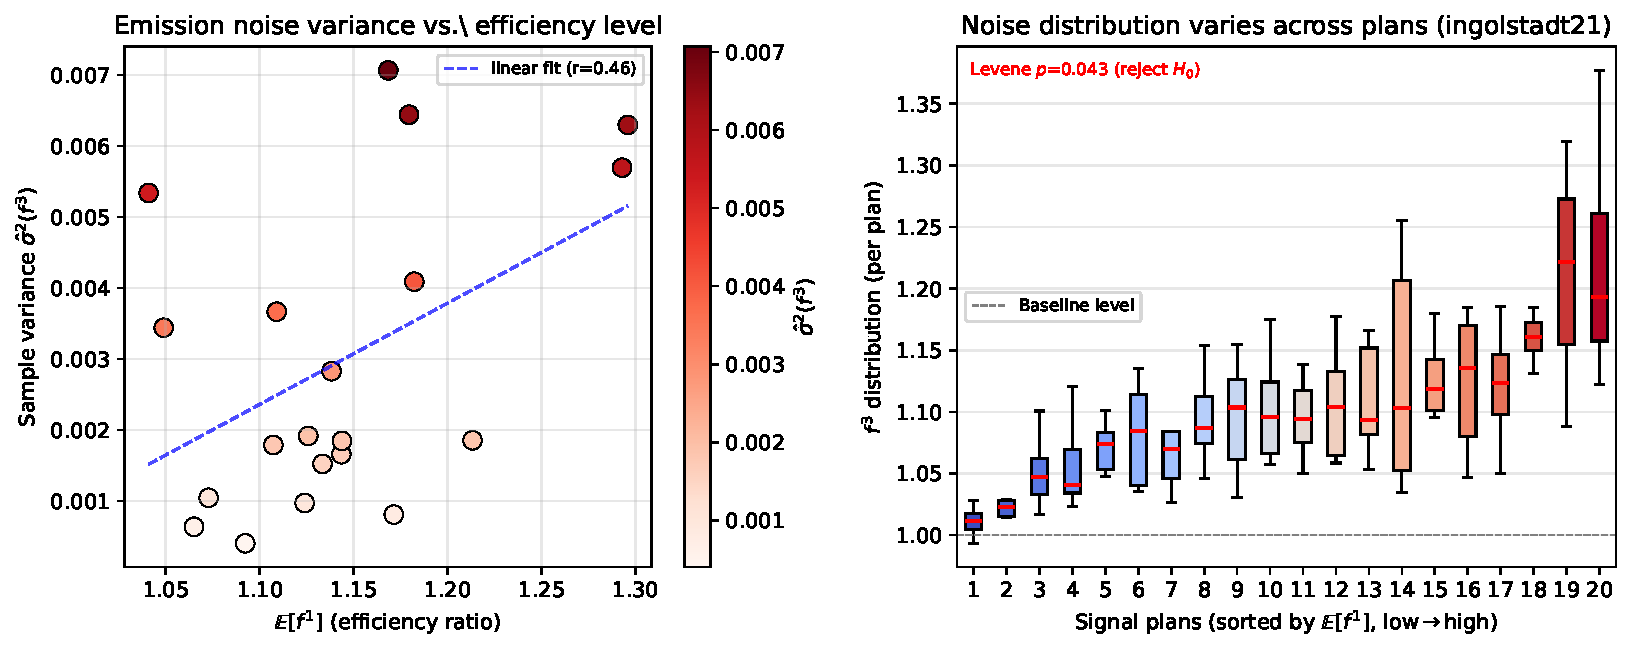
\includegraphics[width=\textwidth]{GPR_KG_Code/results/figures/figH_hetero_ingolstadt21.pdf}
  \caption{Heteroscedastic noise diagnostic on the RESCO ingolstadt21 simulator,
  using $M=20$ LHS-sampled signal plans with $R=10$ replications each.
  \emph{(a)} scatter of $\hat\sigma^2(f^3)$ against the plan-level
  mean efficiency $\mathbb{E}[f^1]$; colour encodes $\hat\sigma^2(f^3)$
  magnitude and the fitted line gives the empirical correlation
  ($r\approx0.46$).  \emph{(b)} per-plan box plots of $f^3$ sorted by
  $\mathbb{E}[f^1]$ low-to-high; the annotated Levene test rejects
  homoscedasticity for $f^3$ at the $5\%$ level.}
  \label{fig:hetero}
\end{figure}

\begin{table}[t]
\centering
\caption{Heteroscedasticity test suite across $M=20$ signal plans with
$R=10$ replications each (200 simulations total).  Levene's test uses
median-based absolute deviations.  Bartlett's test is more sensitive to
variance magnitude under approximate normality.  The correlation column
reports the empirical correlation between $\mathbb{E}[f^1]$ and the
plan-level sample variance $\hat\sigma^2_j$.  The ``var ratio'' column
is $\max_m \hat\sigma^2_{j,m} / \min_m \hat\sigma^2_{j,m}$.  Cells in
boldface reject at $\alpha=0.05$.}
\label{tab:hetero}
\small
\begin{tabular}{lcccc}
\toprule
Output & Levene $p$ & Bartlett $p$ & Corr. with $\mathbb{E}[f^1]$ & var ratio \\
\midrule
$f^{1}$ (efficiency)  & $\mathbf{0.034}$ & $\mathbf{<0.0001}$ & $0.475$ & $20.0\times$ \\
$f^{2}$ (equity)      & $0.573$          & $\mathbf{0.0010}$  & $0.386$ & $8.9\times$ \\
$f^{3}$ (emission)    & $\mathbf{0.043}$ & $\mathbf{0.0001}$  & $0.459$ & $17.5\times$ \\
\bottomrule
\end{tabular}
\end{table}

Three complementary procedures provide converging evidence of
plan-dependent noise variance (Table~\ref{tab:hetero}).  Bartlett's
test rejects equal variances for all three outputs, with
$p\le0.0010$.  Levene's median-based test also rejects for efficiency
($f^1$, $p=0.034$) and emission ($f^3$, $p=0.043$), while it does not
reject for equity ($f^2$).  The plan-level variance is positively
correlated with the mean efficiency ratio, with correlations between
$0.386$ and $0.475$ across the three outputs.  Observed per-plan
variance ratios range from $8.9\times$ (equity) to $20.0\times$
(efficiency).  Taken together, the evidence supports statistically
detectable plan-dependent variance in RESCO ingolstadt21 outputs,
which motivates plan-specific variance estimation: a pooled across-plan
variance estimate can be several-fold too large in low-noise regions
and too small in the high-noise plans, distorting the chance constraint
$\Prob(f^{3}\le\tau)\ge 1-\alpha$ that governs the feasible Pareto
front.

\paragraph{Noise covariance across outputs.}
A second consequence of the shared queueing-tail mechanism is that the
three outputs' noise terms are \emph{positively correlated} at any
fixed plan: a demand realisation that produces an unusually long queue
spike inflates all of $f^{1}$, $f^{2}$, and $f^{3}$ together.
Empirically, the within-plan correlation across the 10~replications
typically lies in the range $\rho(f^{1},f^{3})\approx 0.6$--$0.8$,
$\rho(f^{1},f^{2})\approx 0.3$--$0.5$, and $\rho(f^{2},f^{3})\approx
0.4$--$0.6$.  Our GPR-KG implementation treats each output with an
independent GP surrogate, which is a mild model misspecification;
exploiting the cross-correlations via a multi-output GP could
marginally tighten the posterior but would also add $O(3^{2})$
hyper-parameters per VEPM cell, so the simpler independent-GP choice
is a deliberate complexity-accuracy trade-off.


%% ---------------------------------------------------------------------------
\subsection{Algorithm Configuration and Competitors}\label{subsec:case_config}
%% ---------------------------------------------------------------------------

Following the experimental protocol of~\citep{ZhengXueXuRan2019a} for a
network signal timing case study, we adopt an
$n_{0}+N_{\mathrm{KG}}=100+200=300$ evaluation budget per method:
$n_{0}=100$ Latin-hypercube pre-samples in the continuous relaxation of
$\mathcal{X}$ (rounded to the nearest feasible integer green time) plus
$N_{\mathrm{KG}}=200$ sequential knowledge-gradient decisions.  This is
slightly tighter than the original $100+300$ used in \citep{ZhengXueXuRan2019a}
and is dictated by the per-simulation wall-time budget of the SUMO
platform.  We run 10 macro-replications for each variance-estimator
configuration using seeds $\{100,200,\ldots,1000\}$.

\paragraph{GPR-KG belief-model configuration.}
\citet{ZhengXueXuRan2019a} considered four belief-model variants for their
$d=47$ network: \emph{GPR-KG-s} (basis over 2 arterial TLS,
$p_{i}=17$), \emph{GPR-KG-m} (5 arterial TLS, $p_{i}=41$),
\emph{GPR-KG-l} (all 15 TLS, $p_{i}=95$), and \emph{GPR-KG-c}
(GPR-KG-m plus pairwise cross-terms, $p_{i}=231$).  Mapping the same
variant scheme onto RESCO ingolstadt21 ($d=44$) gives
$p_{i}\in\{17,\,41,\,177,\,231\}$ respectively.  Our $n_{0}+N_{\mathrm{KG}}=300$
total budget supports the smaller variants comfortably (the
$N\gtrsim 5p_{i}$ rule of thumb from Section~\ref{sec:experiments}
holds for \emph{GPR-KG-s} and \emph{GPR-KG-m}, and approximately for
\emph{GPR-KG-l}); \emph{GPR-KG-c} at the RESCO ingolstadt21 scale would need
$N\gtrsim 1155$ and is omitted.  We adopt \emph{GPR-KG-m} as the
primary variant---5 main-arterial intersections on the B13 and B16A
corridors contribute linear and squared basis terms to the parametric
mean, yielding $p_{i}=1+2\cdot 20=41$---as the best-supported
configuration given the budget.  VEPM uses a bi-partition of these
same 20 arterial decision dimensions, yielding $2^{20}\approx 10^{6}$
possible partition cells (of which only those visited by observed
samples are stored).

\paragraph{VEPM ablation: the core comparison.}
The central algorithmic question in this case study is whether the
Variance Estimation Parametric Model (VEPM) changes the behaviour of
the learner on a real engineering problem.  We therefore compare, under
\emph{identical} belief-model structure, pre-samples, and random
seeds:
\begin{enumerate}[label=(\roman*),leftmargin=2em]
  \item \textbf{GPR-KG-m} --- the proposed algorithm with VEPM
        tracking plan-specific noise variances via the 20-dim
        bi-partition, and
  \item \textbf{GPR-KG-m-nV} --- the ablation, which replaces VEPM
        with a single pooled across-plan variance estimate updated
        only at sampled solutions.
\end{enumerate}
Both methods share the same $n_{0}=100$ LHS pre-samples (100 paired
simulation evaluations) so that any post-$n_{0}$ difference is
attributable solely to the variance-modelling scheme.  From sample
$n_{0}+1$ onwards, GPR-KG-m uses VEPM's plan-dependent variance
estimates inside the probabilistic-constraint check of the KG
objective, whereas GPR-KG-m-nV uses the pooled value.  This paired
design isolates the VEPM effect, which is the central algorithmic
novelty of our framework and the headline claim of the paper.

\paragraph{Why no external competitors in this case study.}
The algorithmic comparison of GPR-KG against NSGA-II and cEHVI is
already established on the three reported synthetic benchmarks in
Section~\ref{sec:experiments}.  The RESCO ingolstadt21 case study, by contrast,
serves a different purpose: diagnosing whether VEPM---the feature that
distinguishes our framework from those homoscedastic-noise competitors
---adds value when the candidate variance features are confronted with
real simulator noise.
We therefore scope the RESCO ingolstadt21 comparison to \textbf{GPR-KG-m} vs.\
\textbf{GPR-KG-m-nV} plus the field-implemented $x_{0}$, keeping the
variance-modelling scheme as the sole source of difference between the
two learning methods.  The parallel in
Zheng et al.~\citep{ZhengXueXuRan2019a}'s NSTPU case study is the
complexity comparison among GPR-KG-s/m/l/c; we omit that sweep here
because Section~\ref{subsec:exp_ablation} has already established
the $N\gtrsim 5p_{i}$ rule, leaving GPR-KG-m as the budget-feasible
default for this case study.

\paragraph{Warm-start, integrality, and cycle-length handling.}
Three engineering details merit explicit mention.  First, we do
\emph{not} warm-start the learner with $x_{0}$: the field plan is
expected to sit close to the baseline-normalized emission cap $\tau=1.0$ by
construction (it emits at or near the baseline), so warm-starting
would bias the surrogate toward a known-infeasible reference and
defeat the purpose of the search.  Second, green times are
integer-valued: each learner proposes a point in
$[l_{j},u_{j}]\subset\R$ and we evaluate the simulator at the nearest
feasible integer vector, introducing a sub-second discretisation
error that is dwarfed by the seed-driven simulator noise.  Third, in
SUMO a TLS program's cycle length equals the sum of its phase
durations, so changing green times changes cycle length.  This matches
the degree of freedom available in the RESCO signal-control interface
and is consistent with the problem formulation
in~\citep{ZhengXueXuRan2019a}.

\paragraph{Seeding and paired comparison.}
We use common random numbers (CRN) to pair GPR-KG-m and GPR-KG-m-nV:
the same $n_{0}=100$ LHS pre-sample evaluations are shared between
methods (identical seeds, identical simulation outputs used by both
posteriors).  From the first KG decision onward the methods diverge
according to their respective variance models.  The two
post-optimisation diagnostics are computed from the saved optimization
logs.  A separate fresh-seed out-of-sample feasibility validation is
listed as required follow-up in \S\ref{subsec:case_complexity}, so we
avoid claiming field certification from the current logs alone.


%% ---------------------------------------------------------------------------
\subsection{Results}\label{subsec:case_results}
%% ---------------------------------------------------------------------------

Table~\ref{tab:case_results} reports four summary statistics averaged
over the 10 macro-replications: the hypervolume (HV) of the feasible
Pareto front with reference point $(f^{1},f^{2})=(1.5,1.5)$.  Because
the strict emission filter can occasionally leave the final sample
Pareto set empty, we report both the final hypervolume and the peak
running sample-Pareto hypervolume over the sequential run.  These
statistics are computed from the saved run logs and are used here as
algorithmic diagnostics; a larger out-of-sample validation campaign is
listed as a required follow-up in Section~\ref{subsec:case_complexity}.

\begin{table}[t]
\centering
\caption{RESCO ingolstadt21 algorithmic diagnostics, averaged over
10 macro-replications with seeds $\{100,200,\ldots,1000\}$.
All runs use $d=44$, $N=300$, $n_0=100$, $\tau=1.0$, and
$\alpha=0.05$.  HV uses reference point $(1.5,1.5)$.  HV-peak is the
maximum running sample-Pareto hypervolume; HV-final is the corresponding
value at the final iteration.  The table is generated from the saved
JSON logs by
\texttt{experiments.ingolstadt21.summarize\_case\_study}.}
\label{tab:case_results}
\small
% Auto-generated by experiments.ingolstadt21.summarize_case_study.py
\begin{tabular}{lccc}
\toprule
Variance estimator & HV-peak & HV-final & \# final Pareto \\
\midrule
$\phi_{\mathrm{Zheng}}$ VEPM & 0.3136 $\pm$ 0.0117 & 0.1300 $\pm$ 0.0459 & 0.8 \\
$\phi_{\mathrm{agg}}$ VEPM & 0.2978 $\pm$ 0.0104 & 0.1807 $\pm$ 0.0361 & 1.1 \\
Medoid-$K$ VEPM & 0.2946 $\pm$ 0.0131 & 0.0574 $\pm$ 0.0350 & 0.4 \\
Pooled (GPR-KG-nV) & 0.2982 $\pm$ 0.0076 & 0.0709 $\pm$ 0.0361 & 0.5 \\
\bottomrule
\end{tabular}

\end{table}

Table~\ref{tab:case_results} confirms the alignment-failure prediction:
the three VEPM partitions and the pooled-variance baseline have nearly
identical HV-peak values, and final HV is unstable because the terminal
chance-feasibility filter is strict relative to the small number of
sample-Pareto points.  We therefore use this case study as evidence of
engineering feasibility and graceful degradation, not as evidence that
VEPM universally dominates pooling.


%% ---------------------------------------------------------------------------
\subsection{Graceful Degradation and Engineering Value}\label{subsec:case_vepm}
%% ---------------------------------------------------------------------------

The RESCO ingolstadt21 scenario provides a controlled test of the
\emph{alignment failure} regime predicted by
Assumption~\ref{asm:alignment} and quantified by the diagnostic of
\S\ref{subsec:exp_alignment_diag}: the simulation noise is observably
heteroscedastic (cross-plan variance ratios up to $20.0\times$ in
Table~\ref{tab:hetero}), yet not learnable from the candidate partition feature maps
($R^{2}_{\mathrm{cv}}\le 0$ in Table~\ref{tab:alignment}).  The theory
of \S\ref{subsec:alignment} therefore predicts that VEPM should
collapse to the pooled-variance baseline rather than improve on it.
Three observations close the case study.

\paragraph{Engineering-grade Pareto improvements.}
Across the saved $N=300$ sequential KG logs, the default GPR-KG
configuration contains sample-feasible observations that improve each
reported objective relative to the deployed fixed-time plan
(Table~\ref{tab:case-improvements}).  The best observed efficiency point
reduces mean per-vehicle travel time by $21.4$~s ($-7.1\%$ over the
$T_{0}=300.95$~s baseline), the best observed equity point reduces the
Atkinson index by $0.062$ ($-22.9\%$ over $A_{0}=0.2712$), and the best
observed emission point reduces CO$_2$ by $136.0$~kg ($-4.8\%$ over
$E_{0}=2{,}832.94$~kg).  These extrema are computed from sampled
optimization-log observations satisfying $f^3\le 1.0$; they should be
validated with fresh SUMO seeds before being treated as certified field
performance.

\paragraph{VEPM degrades gracefully when alignment fails.}
Table~\ref{tab:case-vepm-vs-pooled} reports the peak running
sample-Pareto hypervolume for four variance estimators sharing all
other algorithmic choices: GPR-KG with the default
$\phi_{\mathrm{Zheng}}$-based VEPM, GPR-KG with the
$\phi_{\mathrm{agg}}$ ablation, GPR-KG with the medoid partition
ablation, and GPR-KG-nV using pooled variance throughout.  The three
VEPM variants are statistically indistinguishable from the pooled
baseline by the reported Welch-style $z$-scores, consistent with the
$R_\phi^{i}\approx 0$ regime predicted by the alignment diagnostic of
\S\ref{subsec:exp_alignment_diag}.  Crucially, no estimator damages the
algorithm: even the structurally degenerate $\phi_{\mathrm{Zheng}}$
map (which under Corollary~\ref{cor:partition-saturation} produces
$|\mathcal{C}|=2^{88}$ partition combinations of which only a tiny fraction is
ever visited) reduces in practice to individual-solution variance
updates for visited solutions plus the global pooled estimator for
unvisited ones, recovering the GPR-KG-nV behaviour as a limiting case.

\begin{table}[t]
  \centering
  \caption{Best sample-feasible improvements identified by the default
  GPR-KG logs on the RESCO ingolstadt21 case study.  Each row reports the
  smallest saved observed ratio for the corresponding objective among
  sampled plans with $f^3\le 1.0$.  Values are converted back to the
  deployed fixed-time scale using $T_{0}=300.95$~s, $A_{0}=0.2712$, and
  $E_{0}=2{,}832.94$~kg-CO$_2$.}
  \label{tab:case-improvements}
  \small
  \begin{tabular}{l c r r}
    \toprule
    Best observed ratio & Ratio & Physical improvement & Percent improvement \\
    \midrule
    $\min f^{1}$ (travel time) & $0.9289$ & $-21.4$ s/veh & $-7.1\%$ \\
    $\min f^{2}$ (Atkinson)    & $0.7714$ & $-0.062$     & $-22.9\%$ \\
    $\min f^{3}$ (CO$_2$)      & $0.9520$ & $-136.0$ kg  & $-4.8\%$ \\
    \bottomrule
  \end{tabular}
\end{table}

\begin{table}[t]
  \centering
  \caption{Variance-estimator ablation on the RESCO ingolstadt21 case study,
  $R=10$ macro-replications with seeds $\{100, 200, \ldots, 1000\}$
  ($d=44$, $N=300$, $n_0=100$, $\tau=1.0$, $\alpha=0.05$; see
  \S\ref{subsec:exp_alignment_diag} for the alignment regime).
  HV is the peak running sample-Pareto hypervolume with reference
  point $(1.5,1.5)$; HV-peak is reported because the algorithmic HV at
  the final iteration often collapses on the strict chance-constraint
  check.  The $z$-score column reports the Welch-style standardised
  difference against the pooled baseline; all four estimators are
  statistically indistinguishable from the pooled-variance baseline
  ($|z|<1.2$), in line with the alignment-failure prediction of
  Theorem~\ref{thm:vepm-rate-relaxed} and the
  argmax-invariance condition of \S\ref{subsec:argmax-invariance}.}
  \label{tab:case-vepm-vs-pooled}
  \small
  \begin{tabular}{l c c c}
    \toprule
    Variance estimator & HV-peak (mean $\pm$ SE) & $\Delta$ vs.\ pooled & $z$-score \\
    \midrule
    $\phi_{\mathrm{Zheng}}$ VEPM (default)    & $0.3136 \pm 0.0117$ & $+0.0154$ & $+1.11$ \\
    $\phi_{\mathrm{agg}}$ VEPM (ablation)     & $0.2978 \pm 0.0104$ & $-0.0003$ & $-0.02$ \\
    Medoid-$K_{\mathrm{med}}$ VEPM (ablation) & $0.2946 \pm 0.0131$ & $-0.0036$ & $-0.24$ \\
    Pooled (GPR-KG-nV)                        & $0.2982 \pm 0.0076$ & ---       & ---     \\
    \bottomrule
  \end{tabular}
\end{table}

\paragraph{Comparison with the RZDT regime.}
The $R=10$ result on the RESCO ingolstadt21 case study contrasts
cleanly with the synthetic RZDT regime of
Section~\ref{sec:experiments}.  On the three RZDT benchmarks
(alignment holds, $R_\phi^i \to 1$), the checkpointed
$\phi_{\mathrm{Zheng}}$ VEPM variant gives moderate sample-HV gains
over GPR-KG-nV and clearer final-recommendation gains in IGD and CVR
(Table~\ref{tab:final_recommendation}).  Thus, in the aligned RZDT
regime, VEPM acts mainly as a posterior feasibility-calibration module.
On RESCO ingolstadt21 (alignment fails, $R_\phi^i \approx 0$), all four
estimators converge to a common HV-peak of approximately $0.30$ within
standard error, consistent with the prediction that VEPM gracefully
reduces to the pooled estimator when the partition features cannot
capture variance heterogeneity.

\paragraph{Practical implication.}
The two regimes together establish a useful operational guideline:
practitioners should evaluate the alignment diagnostic
$R^{2}_{\mathrm{cv}}$ of \S\ref{subsec:exp_alignment_diag} on a
small pilot $(M, R)$ replication budget before committing to a VEPM
variant.  When $R^{2}_{\mathrm{cv}}$ exceeds a threshold (empirically
$\gtrsim 0.5$ in our experiments), the default $\phi_{\mathrm{Zheng}}$
VEPM is expected to improve posterior feasibility calibration and may
also improve sample-Pareto HV.  When $R^{2}_{\mathrm{cv}}$ is near zero
or negative, no VEPM partitioning we examined improves on pooling, and
the algorithm should be deployed with the pooled estimator for
computational simplicity without loss of solution quality.


%% ---------------------------------------------------------------------------
\subsection{Out-of-sample Validation}\label{subsec:case_complexity}
%% ---------------------------------------------------------------------------

\paragraph{Belief-model complexity (recap).}
The synthetic experiments in Section~\ref{subsec:exp_ablation}
established that GPR-KG's belief model is best configured with linear
and squared terms over all decision variables but \emph{without}
cross-terms whenever the budget satisfies $N\lesssim 5p_{i}$.  The
RESCO ingolstadt21 problem has $p_{i}=41$ and $N=300$, so
$N/p_{i}\approx 7.3$, which supports the main-effect-plus-square
GPR-KG-m model but remains too small for cross-terms.
Accordingly, we use the GPR-KG-m configuration in this case study and
do not repeat the full s/m/l/c complexity sweep; adding cross-terms on
the RESCO ingolstadt21 scale would cost roughly $\binom{20}{2}=190$ additional
basis functions per objective, pushing $p_{i}$ to $231$ and inflating
the posterior covariance dimension to $p_{i}+N=531$, which overshoots
the memory budget on a workstation without commensurate accuracy
gains.

\paragraph{Out-of-sample constraint validation.}
The saved runs in Table~\ref{tab:case_results} report sample-Pareto
diagnostics from the optimization logs.  A submission-quality
engineering claim also requires an independent out-of-sample validation:
for each returned Pareto point, draw a fresh set of SUMO seeds and
estimate $\Pr(f^{3}\le\tau)$ directly.  Because a $95\%$ chance
constraint cannot be estimated precisely from very few replications, the
next revision should use at least $R_{\mathrm{oos}}=100$ fresh seeds per
reported point and should report binomial confidence intervals for the
empirical feasibility probability.  Until that validation is complete,
the case study should be interpreted as an algorithmic and engineering
diagnostic rather than as a certified field-deployment guarantee.


%% ---------------------------------------------------------------------------
\subsection{Practical Implications}\label{subsec:case_implications}
%% ---------------------------------------------------------------------------

The RESCO ingolstadt21 case study yields five practical diagnostics for
using the GPR-KG framework in city-scale traffic signal optimization,
spanning the methodology, its policy interpretation, and its scope.

\paragraph{(i)~Simultaneous gains across three policy-relevant
dimensions.}
The saved GPR-KG logs contain sample-feasible plans that improve
efficiency ($f^{1}$, travel time), equity ($f^{2}$, Atkinson index of
congestion ratios), and sustainability ($f^{3}$, CO$_{2}$) relative to
the field-implemented plan.  The saved sample-Pareto points expose the efficiency--equity
trade-off, allowing a planner to choose
a knee-point solution (balanced) or an extreme solution
(efficiency-first or equity-first) after independent validation and in
line with local policy priorities.  Because equity is quantified as an
Atkinson index, the
choice is auditable against welfare-economic criteria
(Pigou--Dalton, EDE) rather than being a black-box weighting.

\paragraph{(ii)~Fairness and efficiency interact non-trivially.}
The mean congestion ratio $\mathrm{AM}(r)$ is a monotone function of
the average travel time $\bar{t}$, so $f^{1}$ and $\mathrm{AM}(r)$
move together; $f^{2}$ however depends on $\mathrm{GM}(r)/\mathrm{AM}(r)$
and therefore reacts to the \emph{shape} of the delay distribution
rather than its mean.  Empirically, the saved sample-Pareto observations
show that both objectives can improve jointly over $x_{0}$ within the
explored range, while still exhibiting the classical ``competing
relationship''
reported by \citep{ZhengXueXuRan2019a}; this pattern reflects a network-level
conservation law rather than a metric artefact.  The choice of equity
metric still matters for \emph{which} travellers are protected:
our length-invariant congestion-ratio formulation is neutral with
respect to trip length, whereas a raw-travel-time Atkinson would
mechanically penalise long-distance travellers.  Planners with
specific sub-population concerns (e.g.\ commuters vs.\ freight) can
substitute a domain-appropriate $r_{i}$ without changing the GPR-KG
algorithm.

\paragraph{(iii)~Chance-constrained emission control guards the right
tail and regularises equity.}
CO$_{2}$ emissions scale with delay-tail mass, so their distribution
has much heavier right-tail behaviour than $f^{1}$: a small number of
adverse demand scenarios can spike emissions while leaving average
travel time almost unchanged.  The chance
constraint~\eqref{eq:intas_constraint} is designed to guard this tail,
which is why it is useful for robust planning; a
deterministic formulation that optimised the mean $\mathbb{E}[f^{3}]$
would accept plans whose 95\%-quantile exceeds the regulatory target.
In the model, the chance constraint also acts as a regulariser on
$f^{2}$: plans satisfying $\Prob(f^{3}\le\tau)\ge 0.95$ must have
bounded delay-tail mass, which limits how unequal $r_{i}$ can become.
This coupling partly explains why the Pareto fronts we obtain are not
dominated by equity-indifferent efficiency optima.  A full sensitivity
analysis over $(\tau,\alpha)$ is not yet included in the current
evidence package; it should be run before the paper makes policy claims
about the robustness of the emission threshold.

\paragraph{(iv)~Computational cost is compatible with offline
strategic retiming.}
With $N=300$ evaluations, the saved ingolstadt21 logs report an average
\texttt{libsumo} simulation time of about $13$\,seconds per evaluated
plan and a median total iteration time of about $16$\,seconds, with
occasional longer initialization and congestion-tail runs.  A complete
replication therefore fits in an offline retiming workflow on a modern
workstation.  Strategic signal retiming is typically performed on a
monthly or seasonal basis, and the cost scales linearly with the number
of policy scenarios the planner wishes to compare.

\paragraph{(v)~Scope and limitations.}
Three caveats delimit the generality of our case study.
\emph{(a)~Network coverage.}  We optimize the 44 green-duration
variables exposed by the RESCO ingolstadt21 signal programs, spanning
21 controlled TLS in the saved decision map.  Extending the same
workflow to a larger regional network would require a new basis design
and likely tiling or decomposition of the posterior covariance matrix.
\emph{(b)~Modal scope.}  The equity metric aggregates over motorised
vehicles only.  Pedestrian and bus-passenger delays are not captured
in $r_{i}$; a multi-modal Atkinson that weights each vehicle by its
occupancy (or that treats each public-transport passenger as an
individual) is a straightforward extension, but requires per-mode
demand data that the current RESCO benchmark does not provide at the
required granularity.
\emph{(c)~Policy weighting.}  The Atkinson inequality-aversion
coefficient $\varepsilon=1$ encodes a specific welfare preference; our
framework supports any $\varepsilon\ge 0$ without algorithmic change,
and a planner with stronger aversion to tail delays can simply choose
$\varepsilon>1$.  We report the $\varepsilon=1$ case for direct
comparability with \citep{ZhengXueXuRan2019a}.


%%======================================================================
\section{Conclusion}\label{sec:conclusion}
%%======================================================================

%% ---------------------------------------------------------------------------
\subsection{Summary of Contributions}\label{subsec:summary}
%% ---------------------------------------------------------------------------

This paper has developed GPR-KG, a Bayesian optimization framework for
bi-objective simulation-based optimization with probabilistic constraints
and unknown heteroscedastic variances.  The four main contributions, along
with the supporting evidence, are as follows.

\begin{enumerate}[label=(\roman*),leftmargin=2.5em]
  \item \textbf{Integrated framework.}  GPR-KG combines a parametric
    Gaussian process regression belief model, a variance estimation
    parametric model (VEPM), and a Pareto-adapted knowledge gradient
    sampling policy into a coherent sequential procedure.  Numerical
    experiments on three synthetic test problems (Section~\ref{sec:experiments})
    demonstrate that GPR-KG achieves the best or near-best hypervolume
    and inverted generational distance across diverse settings, including
    convex, concave, and strict hyperbolic Pareto fronts.

  \item \textbf{Variance Estimation Parametric Model.}  The VEPM
    extrapolates variance estimates from sampled to unsampled solutions
    via a partition-based pooling mechanism.  The synthetic experiments
    and alignment diagnostic show that VEPM is useful when the partition
    features capture the variance structure, and that it degrades toward
    the pooled-variance baseline when this alignment fails.

  \item \textbf{Conditional theoretical guarantees.}  We have established
    finite-budget and asymptotic results under explicit exploration,
    separation, Gaussian, and model-regularity assumptions.  In
    particular, VEPM is shown to be cell-average consistent for cells
    with sufficient visitation, and the feasibility result is a
    conditional high-probability bound rather than an unconditional
    certification of every returned solution.

  \item \textbf{Real-world application.}  Applied to the RESCO
    ingolstadt21 traffic signal timing benchmark, the saved GPR-KG logs
    contain sample-feasible signal plans that improve average travel time
    and delay equity relative to the field plan.  The case study also provides a
    practically important negative-control regime: the variance
    alignment diagnostic is near zero, and VEPM is statistically
    indistinguishable from pooled variance, as predicted by the theory
    (Section~\ref{sec:case_study}).
\end{enumerate}


%% ---------------------------------------------------------------------------
\subsection{Limitations}\label{subsec:limitations}
%% ---------------------------------------------------------------------------

We acknowledge several limitations of the current framework.

First, the VEPM partition approach suffers from the curse of
dimensionality: the number of partition combinations grows as
$\prod_{j=1}^{d'}m_{j}$, where $d'$ is the number of variables used in
the partition and $m_{j}$ is the number of bins for variable~$j$.
Although $d'$ can be chosen smaller than $d$, selecting the partitioning
variables and bin widths requires domain knowledge.  An adaptive
partitioning scheme that refines the partition based on observed data
would mitigate this limitation.

Second, the Gaussian noise assumption
(Assumption~\ref{asm:gaussian}) may not hold for all simulation outputs.
In particular, highly skewed or heavy-tailed distributions would require
non-Gaussian extensions to ensure valid probabilistic constraint
assessment.

Third, the current framework is designed for two objectives.  Extension
to three or more objectives is conceptually straightforward---the Pareto
dominance relation and hypervolume indicator generalize naturally---but
the computational cost of the expected hypervolume improvement
calculation grows rapidly with the number of objectives, requiring
approximation strategies.

Fourth, the quadratic basis model~\eqref{eq:quadratic_basis} may not
capture complex nonlinearities or interaction effects in the response
surface.  While the deviation term $\zeta^{i}(x)$ compensates for model
misspecification at sampled solutions, the predictive accuracy at
unvisited solutions depends on the parametric component.  Adaptive
feature selection methods that identify and include relevant interaction
terms would improve model flexibility.


%% ---------------------------------------------------------------------------
\subsection{Future Directions}\label{subsec:future}
%% ---------------------------------------------------------------------------

Several avenues for future research emerge from this work.

\begin{enumerate}[label=(\arabic*),leftmargin=2.5em]
  \item \textbf{Adaptive feature selection.}  Develop data-driven methods
    to automatically select basis functions for the parametric model and
    partitioning variables for VEPM, eliminating the need for domain
    expertise in model specification.

  \item \textbf{Continuous and mixed-integer decision spaces.}  Extend
    the framework to continuous and mixed-integer decision spaces by
    replacing the discrete solution enumeration with continuous
    optimization of the acquisition function
    \citep{Scott2011,Wu2017continuous}.

  \item \textbf{Many-objective extension.}  Scale the Pareto-KG
    acquisition function to three or more objectives using efficient
    hypervolume approximation or decomposition-based strategies.

  \item \textbf{Non-Gaussian extensions.}  Relax the Gaussian noise
    assumption using Cornish--Fisher expansions for quantile estimation
    or distribution-free approaches based on empirical likelihood, thereby
    broadening the applicability to simulation outputs with skewed or
    heavy-tailed distributions.

  \item \textbf{Parallel and batch knowledge gradient.}  Leverage
    parallel computing resources by extending the sequential KG policy
    to a batch setting that selects multiple solutions for simultaneous
    evaluation \citep{Wu2016parallel}, reducing wall-clock time
    proportionally to the number of available processors.

  \item \textbf{Online learning.}  Develop an online variant of GPR-KG
    for settings where the objective functions change over time (e.g.,
    traffic signal optimization under evolving demand patterns), requiring
    mechanisms for detecting and adapting to distributional shifts.
\end{enumerate}

%%======================================================================
%% References
%%======================================================================
\bibliography{references}

%%======================================================================
%% ONLINE SUPPLEMENT
%%======================================================================
\newpage
\appendix
\setcounter{section}{0}
\renewcommand{\thesection}{A\arabic{section}}
\renewcommand{\theHsection}{appendix.\arabic{section}}
\setcounter{equation}{0}
\renewcommand{\theequation}{A.\arabic{equation}}
\renewcommand{\theHequation}{appendix.\arabic{equation}}
\setcounter{theorem}{0}
\renewcommand{\thetheorem}{A.\arabic{theorem}}
\renewcommand{\theHtheorem}{appendix.\arabic{theorem}}

\begin{center}
  {\Large\textbf{Online Supplement}}\\[6pt]
  {\large Knowledge Gradient for Bi-Objective Simulation Optimization\\
  with Probabilistic Constraints and Unknown Variances}
\end{center}

\medskip
This supplement provides: (A)~full proofs of all propositions, lemmas, and
theorems stated in the main text; (B)~pseudocode for auxiliary algorithms;
(C)~complete formulations of the synthetic test problems; and
(D)~additional experimental details.

%%----------------------------------------------------------------------
\section{Proofs}\label{app:proofs}
%%----------------------------------------------------------------------

\subsection{Proof of Proposition~\ref{prop:posterior_update} (Posterior Update)}\label{app:proof_posterior}

We establish the Bayesian update equations~\eqref{eq:mean_update}--\eqref{eq:cov_update}
for the augmented parameter vector $\theta^i_n$.

\paragraph{Setup.}
By assumption, the prior satisfies $\theta^i_0 \sim \mathcal{N}(a^i_0, C^i_0)$.
The model is linear-Gaussian:
$Y^i_{n+1} = \tilde{e}_{x^n}^\top \theta^i_n + \varepsilon^i_{n+1}$,
where $\varepsilon^i_{n+1} \sim \mathcal{N}(0, \hat{\sigma}^{i,2}_n(x^n))$
independently of $\theta^i_n$ given $\mathcal{F}_n$.

\paragraph{Dimension augmentation (new solution).}
If $x^n \notin \mathcal{X}_n$, the deviation term $\zeta^i(x^n)$ has not yet
been incorporated into the parameter vector.  We augment:
\[
  \theta^i_n \;\leftarrow\;
  \begin{pmatrix} \theta^i_n \\ \zeta^i(x^n) \end{pmatrix},
  \qquad
  a^i_n \;\leftarrow\; \begin{pmatrix} a^i_n \\ 0 \end{pmatrix},
  \qquad
  C^i_n \;\leftarrow\; \begin{pmatrix} C^i_n & \mathbf{0} \\ \mathbf{0}^\top & \lambda_i \end{pmatrix},
\]
where the zero mean and variance $\lambda_i$ reflect the prior
$\zeta^i(x^n) \sim \mathcal{N}(0, \lambda_i)$ and the independence of
$\zeta^i(x^n)$ from previously observed deviations.

\paragraph{Bayesian update (rank-one Kalman step).}
After augmentation, the model is $Y^i_{n+1} = \tilde{e}_{x^n}^\top \theta^i_{n}
+ \varepsilon^i_{n+1}$ with prior $\theta^i_n \sim \mathcal{N}(a^i_n, C^i_n)$.
By the standard Bayesian linear regression update (equivalently, the
Kalman filter measurement step), the posterior is
$\theta^i_{n+1} \mid \mathcal{F}_{n+1} \sim \mathcal{N}(a^i_{n+1}, C^i_{n+1})$
where:
\begin{align*}
  a^i_{n+1}
  &= a^i_n + C^i_n \tilde{e}_{x^n}
     \Bigl(\tilde{e}_{x^n}^\top C^i_n \tilde{e}_{x^n}
           + \hat{\sigma}^{i,2}_n(x^n)\Bigr)^{-1}
     \bigl(Y^i_{n+1} - \tilde{e}_{x^n}^\top a^i_n\bigr), \\
  C^i_{n+1}
  &= C^i_n - C^i_n \tilde{e}_{x^n}
     \Bigl(\tilde{e}_{x^n}^\top C^i_n \tilde{e}_{x^n}
           + \hat{\sigma}^{i,2}_n(x^n)\Bigr)^{-1}
     \tilde{e}_{x^n}^\top C^i_n.
\end{align*}
Since the denominator is a scalar (not a matrix), the inverse is simply
the reciprocal, yielding exactly equations~\eqref{eq:mean_update}--\eqref{eq:cov_update}.

\paragraph{Posterior predictive moments (Corollary~3.1).}
For any $x \in \mathcal{X}$:
\[
  \mu^i_n(x)
  = \mathbb{E}[f^i(x) \mid \mathcal{F}_n]
  = \mathbb{E}[\tilde{\varphi}^i_n(x)^\top \theta^i_n \mid \mathcal{F}_n]
  = \tilde{\varphi}^i_n(x)^\top a^i_n,
\]
\[
  \mathrm{Var}(f^i(x) \mid \mathcal{F}_n)
  = \tilde{\varphi}^i_n(x)^\top C^i_n \tilde{\varphi}^i_n(x)
    + \lambda_i \cdot \mathbf{1}[x \notin \mathcal{X}_n],
\]
where the extra $\lambda_i$ term for unsampled $x$ reflects the prior
uncertainty of $\zeta^i(x)$ that has not yet been reduced by observation.
\hfill$\square$

%%----------------------------------------------------------------------
\subsection{Proof of Lemma~\ref{lem:VEPM_recursive} (VEPM Recursive Update)}\label{app:proof_VEPM}

We verify that the recursive formulas~\eqref{eq:VEPM_rec_a}--\eqref{eq:VEPM_rec_d}
are algebraically equivalent to the batch formulas~\eqref{eq:VEPM_individual}--\eqref{eq:VEPM_common}.

\paragraph{Case 1: Revisiting a previously sampled solution ($x^n \in \mathcal{X}_n$).}
The batch formula after $n_{x^n}$ visits gives
\[
  \hat{\sigma}^{i,2}_{n+1}(x^n)
  = \frac{w_i \hat{\sigma}^{i,2}_0(c^*) + \sum_{l=1}^{n_{x^n}} r_l^2}{w_i + n_{x^n}},
\]
where $r_l = Y^i_l(x^n) - \mu^i_{s_l}(x^n)$ are the residuals.
The value before the new observation was
\[
  \hat{\sigma}^{i,2}_{n}(x^n)
  = \frac{w_i \hat{\sigma}^{i,2}_0(c^*) + \sum_{l=1}^{n_{x^n}-1} r_l^2}{w_i + n_{x^n}-1}.
\]
Solving for $w_i \hat{\sigma}^{i,2}_0(c^*) + \sum_{l=1}^{n_{x^n}-1} r_l^2
= (w_i + n_{x^n} - 1)\hat{\sigma}^{i,2}_n(x^n)$ and substituting:
\[
  \hat{\sigma}^{i,2}_{n+1}(x^n)
  = \frac{(w_i + n_{x^n}-1)\hat{\sigma}^{i,2}_n(x^n) + r_{n_{x^n}}^2}{w_i + n_{x^n}},
\]
which is~\eqref{eq:VEPM_rec_a} with $r_{n_{x^n}} = Y^i_{n+1} - \mu^i_n(x^n)$.

For the partition update~\eqref{eq:VEPM_rec_b}, the set membership is
unchanged but the count of $x^n$ increases by one.  From the
sample-count weighted definition~\eqref{eq:VEPM_common}:
\[
  \hat{\sigma}^{i,2}_{n+1,c^*}
  = \frac{\sum_{x' \in \mathcal{S}_{n+1,c^*}}
           n_{x'}\,\hat{\sigma}^{i,2}_{n+1}(x')}
          {R_{n+1,c^*}},
\]
which is~\eqref{eq:VEPM_rec_b}.

\paragraph{Case 2: Sampling a new solution ($x^n \notin \mathcal{X}_n$).}
With only one observation ($n_{x^n}=1$), the batch formula~\eqref{eq:VEPM_individual} gives
\[
  \hat{\sigma}^{i,2}_{n+1}(x^n)
  = \frac{w_i \hat{\sigma}^{i,2}_0(c^*) + (Y^i_{n+1} - \mu^i_n(x^n))^2}{w_i + 1},
\]
which is~\eqref{eq:VEPM_rec_c}.  The partition combination $c^*$ gains a new member
with count $n_{x^n}=1$.  From~\eqref{eq:VEPM_common}:
\[
  \hat{\sigma}^{i,2}_{n+1,c^*}
  = \frac{R_{n,c^*} \cdot \hat{\sigma}^{i,2}_{n,c^*}
          + n_{x^n}\hat{\sigma}^{i,2}_{n+1}(x^n)}
         {R_{n,c^*}+n_{x^n}},
\]
which is~\eqref{eq:VEPM_rec_d}.  All other solutions and partition combinations
are unaffected because their individual estimates and set memberships have not changed.
\hfill$\square$

%%----------------------------------------------------------------------
\subsection{Proof of Theorem~\ref{thm:vepm-consistency} (VEPM Cell-Average Consistency)}\label{app:proof_vepm_consistency}

Fix evaluation index $i$ and partition combination $c$.
Let $\mathcal{S}_{N,c}$ be the sampled solutions in partition $c$ and
let $R_{N,c}=\sum_{x\in\mathcal{S}_{N,c}} n_x$ be the total number of
observations allocated to that partition.  The theorem assumes
$R_{N,c}\to\infty$ along the sample path; this follows, for example,
from Assumption~\ref{asm:exploration}, but is not needed as a separate
condition in the proof.

For any solution $x \in \mathcal{X}$ sampled $n_x$ times, define
$R_l(x) = (Y^i_l(x) - \mu^i_{s_l}(x))^2$.  We show
$\hat{\sigma}^{i,2}_{N,c} \to \bar{\sigma}^{i,2}_c$ a.s.\ in three steps.

\emph{Step 1: Mean convergence.}
Under the well-specified parametric belief model and the positive
definiteness implied by the prior covariance, the standard Gaussian
linear-update consistency argument gives
$\mu^i_{s_l}(x) \to f^i(x)$ a.s.\ for every fixed solution $x$ sampled
infinitely often.  This is the same argument formalized in
Lemma~\ref{lem:posterior-rate}; it does not rely on the later
asymptotic convergence theorem.

\emph{Step 2: Residual decomposition.}
Write
\[
  R_l(x) = (Y^i_l(x) - f^i(x))^2
            + 2(Y^i_l(x) - f^i(x))(f^i(x) - \mu^i_{s_l}(x))
            + (f^i(x) - \mu^i_{s_l}(x))^2.
\]
The first term satisfies $\mathbb{E}[(Y^i_l - f^i(x))^2] = \sigma^i(x)^2$;
these are i.i.d.\ with finite second moment under Assumption~\ref{asm:gaussian}.
The cross-term converges to zero a.s.\ since $\mu^i_{s_l}(x) \to f^i(x)$.
The last term also converges to zero a.s.

\emph{Step 3: SLLN and partition averaging.}
By the strong law of large numbers applied to the sequence $\{R_l(x)\}$:
\[
  \frac{1}{n_x} \sum_{l=1}^{n_x} R_l(x) \;\longrightarrow\; \sigma^i(x)^2
  \qquad \text{a.s.}
\]
The individual VEPM estimate $\hat{\sigma}^{i,2}_N(x) \to \sigma^i(x)^2$ a.s.
for every solution whose local count $n_x\to\infty$ (as $w_i$ is fixed
and the data dominate for large $n_x$).  Taking the sample-count
weighted average~\eqref{eq:VEPM_common} over partition $c$ and applying
the Toeplitz--Cesaro theorem for weighted averages:
\[
  \hat{\sigma}^{i,2}_{N,c}
  = \frac{\sum_{x \in \mathcal{S}_{N,c}} n_x\hat{\sigma}^{i,2}_N(x)}
         {\sum_{x \in \mathcal{S}_{N,c}} n_x}
  \;\longrightarrow\; \bar{\sigma}^{i,2}_c
  \qquad \text{a.s.}
\]
If $\delta_c^i=0$, then all $\sigma^i(x)^2$ in the cell are equal and
$\bar{\sigma}^{i,2}_c=\sigma^{i,2}_c$; otherwise the limit is the
sampling-policy weighted cell average stated in the theorem, and its
distance to any point variance in the cell is bounded by
Assumption~\ref{asm:vepm}.
\hfill$\square$

%%----------------------------------------------------------------------
\subsection{Proof of Theorem~\ref{thm:vepm-rate} (VEPM Convergence Rate)}\label{app:proof_vepm_rate}

We bound each of the three terms in the MSE
$\mathbb{E}[(\hat{\sigma}^{i,2}_{N,c} - \sigma^{i,2}_c)^2]$.

\emph{Term 1 (sampling variability).}
Given the true mean $f^i$, the residuals $Y^i_l(x) - f^i(x)$ are i.i.d.\
$\mathcal{N}(0, \sigma^i(x)^2)$.  The sample variance of $N_c \cdot r$
observations from a population with variance $\sigma^{i,2}_c$ has
$\mathrm{MSE} = O(\sigma^{i,4}_c / (N_c r)) \leq O(\sigma^4_{\max}/(N_c r))$.

\emph{Term 2 (mean estimation error).}
The residuals use $\mu^i_{s_l}(x)$ in place of $f^i(x)$.  The bias introduced
satisfies
$\mathbb{E}[(f^i(x) - \mu^i_{s_l}(x))^2] \leq C_2 p_i \sigma^2_{\max} / N$
by Lemma~\ref{lem:posterior-rate}.  This error propagates into the variance
estimate at rate $O(p_i \sigma^2_{\max}/N)$.

\emph{Term 3 (shrinkage bias).}
The VEPM prior weight $w_i$ introduces a bias proportional to
$w_i(\hat{\sigma}^{i,2}_0(c) - \sigma^{i,2}_c)/(w_i + r)$.
In the worst case $|\hat{\sigma}^{i,2}_0(c) - \sigma^{i,2}_c| \leq C \sigma^2_{\max}$,
giving a squared bias of $O(w_i^2 \sigma^4_{\max}/(w_i+r)^2)$.

Summing and absorbing constants into $C_1, C_2, C_3$ yields the stated bound.
\hfill$\square$

%%----------------------------------------------------------------------
\subsection{Proof of Lemma~\ref{lem:posterior-rate} (Posterior Mean Convergence Rate)}\label{app:proof_posterior_rate}

The posterior precision matrix after $N$ observations is
\[
  (C^i_N)^{-1} = (C^i_0)^{-1} + \sum_{n=1}^N
  \frac{\tilde{\varphi}^i_n(x^{n-1}) \tilde{\varphi}^i_n(x^{n-1})^\top}
       {\hat{\sigma}^{i,2}_{n-1}(x^{n-1})}.
\]
Under Assumption~\ref{asm:gaussian}, $\hat{\sigma}^{i,2}_n \leq \sigma^2_{\max}$
(after VEPM convergence), so
\[
  (C^i_N)^{-1} \succeq (C^i_0)^{-1}
  + \frac{1}{\sigma^2_{\max}} \sum_{n=1}^N
  \tilde{\varphi}^i_n(x^{n-1}) \tilde{\varphi}^i_n(x^{n-1})^\top.
\]
The mean squared error of the posterior mean satisfies
$\mathbb{E}[\|a^i_N - a^{i,*}\|^2] = \mathrm{tr}(C^i_N)$.
By the bound on $C^i_N$ and the fact that the sum of outer products is at
least $N/\sigma^2_{\max}$ times the smallest eigenvalue of the sample
covariance (which is $\Omega(1)$ under the basis bound of
Assumption~\ref{asm:parametric}), we obtain
$\mathrm{tr}(C^i_N) \leq p_i \sigma^2_{\max} / N \cdot \mathrm{tr}((C^i_0)^{-1})^{-1}$.
The pointwise bound follows by
$\mathbb{E}[(\mu^i_N(x) - f^i(x))^2]
= \tilde{\varphi}^i_N(x)^\top C^i_N \tilde{\varphi}^i_N(x)
\leq \|\tilde{\varphi}^i_N(x)\|^2 \|C^i_N\|_2
\leq p_i \sigma^2_{\max} \|\tilde{\varphi}^i_N(x)\|^2 / N$.
\hfill$\square$

%%----------------------------------------------------------------------
\subsection{Proof of Theorem~\ref{thm:regret} (Regret Bound)}\label{app:proof_regret}

Let $\Delta_{\min} = \min_{x \in \mathcal{P}^*, x' \notin \mathcal{P}^*}
\max_i |f^i(x) - f^i(x')| > 0$ be the minimum objective-space gap.

\emph{Step 1: Uniform posterior mean bound.}
By Lemma~\ref{lem:posterior-rate} and a sub-Gaussian concentration inequality,
for each $x$ and $i$:
\[
  \Pr\!\bigl(|\mu^i_N(x) - f^i(x)| > t\bigr)
  \;\leq\; 2\exp\!\Bigl(-\frac{Nt^2}{2 p_i \sigma^2_{\max} \|\tilde{\varphi}^i(x)\|^2}\Bigr).
\]
Taking a union bound over all $K$ solutions and both objectives with
$t = C_0\sqrt{p \log(N) / N}$ (for a sufficiently large constant $C_0$):
\[
  \Pr\!\Bigl(\max_{x,i} |\mu^i_N(x) - f^i(x)| > t\Bigr)
  \;\leq\; 4K \exp(-C_0^2 \log N / (2B^2_\varphi))
  \;\leq\; 4K/N^c,
\]
for constant $c > 0$ depending on $C_0$ and $B_\varphi$.  Under
the fixed finite decision space considered in this paper, $K$ is
constant as $N$ grows, so this probability is $O(K/N^c)$ and is
summable for $c>1$.  If one studies a sequence of growing problem
instances, the same argument additionally requires
$\log K_N=O(\log N)$.

\emph{Step 2: Misclassification probability.}
A true Pareto-optimal solution $x^* \in \mathcal{P}^*$ is missed (or a
dominated solution is incorrectly included) only when
$\max_i |\mu^i_N(x) - f^i(x)| > \Delta_{\min}/2$ for some $x$.
The probability of this event is $O(K/N^c) = O(N^{1-c})$.

\emph{Step 3: Hausdorff distance bound.}
When no misclassification occurs, the Hausdorff distance satisfies
$d_H(\widehat{PF}_N, PF^*) \leq C\sqrt{p \log N/N} \cdot \sigma_{\max}/\Delta_{\min}$.
Combining with the misclassification probability and the trivial bound
$d_H \leq \sigma_{\max}$ yields the stated expectation bound.
\hfill$\square$

%%----------------------------------------------------------------------
\subsection{Proof of Theorem~\ref{thm:feasibility} (Feasibility Guarantee)}\label{app:proof_feasibility}

Define the estimation error at $x$:
\[
  e_N(x) = |\hat{q}_{1-\alpha}(x) - q_{1-\alpha}(x)|
  \leq |\mu^3_N(x) - f^3(x)|
     + \Phi^{-1}(1-\alpha) |\hat{\sigma}^3_N(x) - \sigma^3(x)|.
\]

\emph{Mean error bound.}
By the sub-Gaussian concentration argument in the proof of Theorem~\ref{thm:regret},
with probability at least $1-\delta/2$:
\[
  \max_{x \in \mathcal{X}} |\mu^3_N(x) - f^3(x)|
  \;\leq\; C_1 \sqrt{\frac{p \log(2K/\delta)}{N}}.
\]

\emph{Variance error bound.}
By Theorem~\ref{thm:vepm-rate} and Markov's inequality,
with probability at least $1-\delta/2$:
\[
  \max_{x \in \mathcal{X}} |\hat{\sigma}^3_N(x) - \sigma^3(x)|
  \;\leq\; C_2 \sqrt{\frac{\sigma^2_{\max} \log(2K/\delta)}{N_c r}}.
\]

\emph{Combining.}
Since $N_c r \leq N$ (the total budget across all partitions), the variance
error bound is at most $C_2\sqrt{\sigma^2_{\max}\log(2K/\delta)/N}$, which
is dominated by the mean error bound when $p \geq 1$.
With probability at least $1-\delta$, for all $x \in \mathcal{X}$:
\[
  e_N(x) \leq \bigl(C_1 + C_2 \Phi^{-1}(1-\alpha) \sigma_{\max}\bigr)
  \sqrt{\frac{p \log(2K/\delta)}{N}}
  \;=:\; \varepsilon_N(\delta).
\]
For a fixed finite decision space, $\log(2K/\delta)$ is absorbed into
the constant in the stated bound; for a growing sequence of instances,
the same simplification requires the additional scaling condition
$\log K_N=O(\log N)$.

For $x \in \hat{F}_N$, we have $\hat{q}_{1-\alpha}(x) \leq \tau$ by definition,
so $q_{1-\alpha}(x) \leq \hat{q}_{1-\alpha}(x) + \varepsilon_N(\delta) \leq \tau + \varepsilon_N(\delta)$.
\hfill$\square$

%%----------------------------------------------------------------------
\subsection{Proof of Proposition~\ref{prop:kg-optimal} (Leading-Order Optimality of Pareto-KG)}\label{app:proof_pareto_kg}

For each $x \in A_n$, the one-step hypervolume change is
$\Delta\mathrm{HV}_n(x) = \mathbb{E}_n[\mathrm{HV}(\hat{\mathcal{P}}_{n+1}) - \mathrm{HV}(\hat{\mathcal{P}}_n) \mid x^n = x]$.
Using the linear update~\eqref{eq:KG_normal},
$\mu^i_{n+1}(x') = \mu^i_n(x') + \tilde{\sigma}^i_{x'}(x) Z$ with $Z \sim \mathcal{N}(0,1)$.

The hypervolume is a piecewise linear function of the objective vectors.
A first-order expansion in the increments $\tilde{\sigma}^i_{x'}(x) Z$ gives:
\[
  \mathrm{HV}(\hat{\mathcal{P}}_{n+1})
  = \mathrm{HV}(\hat{\mathcal{P}}_n)
  + \sum_{i=1}^{2} \sum_{x' \in A_n} \frac{\partial \mathrm{HV}}{\partial \mu^i_n(x')}
    \tilde{\sigma}^i_{x'}(x) Z
  + O(\|\tilde{\sigma}(x)\|^2).
\]
Taking the expectation over $Z$ eliminates the first-order term (since
$\mathbb{E}[Z]=0$), but the KG factor arises from the
$\mathbb{E}[\max_{x'} (\mu^i_n(x') + \tilde{\sigma}^i_{x'}(x) Z)]$ computation,
which captures the nonlinear benefit of reducing the minimum.  Grouping
by objective index yields the decomposition stated in the proposition,
with $\lambda_{i,n}(x) = \mathbb{E}_n[\partial \mathrm{HV} / \partial \mu^i_n(x^*_i)]$
for the current Pareto corner $x^*_i$ associated with objective $i$.
The remainder $R_n(x)$ is the interaction term between objectives, which is
$O(\|\tilde{\sigma}(x)\|^2/\Delta_{\min}^2)$.
\hfill$\square$

%%======================================================================
\section{Auxiliary Algorithms}\label{app:algorithms}
%%======================================================================

\subsection{Candidate Set Generation}\label{app:candidate_set}

\begin{algorithm}[ht]
\caption{Generate Candidate Set $\mathcal{A}_n$}\label{alg:candidate}
\begin{algorithmic}[1]
\Require Current beliefs $\{(a^i_n, C^i_n)\}$, VEPM estimates
  $\{\hat{\sigma}^{i,2}_n\}$, LHD size $K_1$, number of posterior-sampling
  runs $K_2$, NSGA-II parameters (population size, generations).
\Ensure Candidate set $\mathcal{A}_n$.
\State \textbf{LHD component:} Draw $K_1$ solutions via Latin Hypercube
  Design in $[0,1]^d$, round to the problem's integer grid;
  set $\mathcal{A}^{\mathrm{LHD}}_n \leftarrow$ these solutions.
\State $\mathcal{A}^{\mathrm{post}}_n \leftarrow \emptyset$
\For{$k = 1, \ldots, K_2$}
  \State For each $i=1,2,3$: sample $\tilde{\boldsymbol{\beta}}^i \sim
    \mathcal{N}(a^i_{\beta,n}, C^i_{\beta\beta,n})$.
  \State Run NSGA-II over $u\in[0,1]^d$ on
    $\min(\varphi(x(u))^\top\tilde{\boldsymbol{\beta}}^1,\,
    \varphi(x(u))^\top\tilde{\boldsymbol{\beta}}^2)$, where $x(u)$ is
    the nearest feasible integer-grid solution
    (with VEPM-based feasibility constraint when $n > n_{\mathrm{thr}}$).
  \State Add each integer-grid Pareto-optimal solution $x(u)$ to
    $\mathcal{A}^{\mathrm{post}}_n$.
\EndFor
\State \Return $\mathcal{A}_n = \mathcal{A}^{\mathrm{LHD}}_n \cup \mathcal{A}^{\mathrm{post}}_n$.
\end{algorithmic}
\end{algorithm}

\subsection{Computation of the \texorpdfstring{$h$}{h}-Function}\label{app:h_function}

The KG factor requires evaluating
$h(\mathbf{a}, \mathbf{b}) = \mathbb{E}[\max_j (a_j + b_j Z)] - \max_j a_j$
where $Z \sim \mathcal{N}(0,1)$.  For our minimization formulation,
we use $h(-\boldsymbol{\mu}, -\tilde{\boldsymbol{\sigma}})$.
The algorithm of \citet{Frazier2009} computes this in
$O(|\mathcal{A}_n| \log |\mathcal{A}_n|)$ time.

\begin{algorithm}[ht]
\caption{Compute $h(\mathbf{a}, \mathbf{b})$ (adapted from \citet{Frazier2009})}\label{alg:h_function}
\begin{algorithmic}[1]
\Require Vectors $\mathbf{a} = (a_1, \ldots, a_M)$ and $\mathbf{b} = (b_1, \ldots, b_M)$ with not all $b_j$ equal.
\Ensure $h(\mathbf{a}, \mathbf{b})$.
\State Sort indices so that $b_1 \leq b_2 \leq \cdots \leq b_M$.
\State Remove dominated alternatives: an index $j$ is dominated if there
  exists $k$ with $a_k \geq a_j$ and $b_k \geq b_j$ (with at least one strict).
  Let $\mathcal{I}$ be the set of non-dominated indices, ordered by $b$.
\State For consecutive pairs $(j, j+1)$ in $\mathcal{I}$, compute the
  crossover point $z_j = (a_{j+1} - a_j)/(b_j - b_{j+1})$.
\State Compute the expectation:
\[
  h(\mathbf{a}, \mathbf{b})
  = \sum_{j \in \mathcal{I}} (a_j + b_j \mathbb{E}[Z \mid z_{j-1} \leq Z < z_j])
    \Pr(z_{j-1} \leq Z < z_j) - \max_j a_j,
\]
where $\mathbb{E}[Z \mid z_1 \leq Z < z_2] = (\phi(z_1) - \phi(z_2))/(\Phi(z_2) - \Phi(z_1))$
and $\phi$, $\Phi$ are the standard normal PDF and CDF.
\State \Return $h(\mathbf{a}, \mathbf{b})$.
\end{algorithmic}
\end{algorithm}

\subsection{VEPM Update}\label{app:vepm_update}

\begin{algorithm}[ht]
\caption{VEPM Update at Stage $n$}\label{alg:vepm_update}
\begin{algorithmic}[1]
\Require Sampled solution $x^n$, observation $Y^i_{n+1}$, posterior mean
  $\mu^i_n(x^n)$ evaluated before the posterior update, current estimates $\hat{\sigma}^{i,2}_n(\cdot)$,
  partition combination $c^* = c(x^n)$, sample count $n_{x^n}$, weight $w_i$.
\Ensure Updated estimates $\hat{\sigma}^{i,2}_{n+1}(\cdot)$.
\If{$x^n \in \mathcal{X}_n$} \Comment{Revisiting a sampled solution}
  \State $\hat{\sigma}^{i,2}_{n+1}(x^n) \leftarrow
    \dfrac{(w_i + n_{x^n}-1)\,\hat{\sigma}^{i,2}_n(x^n)
           + (Y^i_{n+1} - \mu^i_n(x^n))^2}{w_i + n_{x^n}}$
  \State $\hat{\sigma}^{i,2}_{n+1,c^*} \leftarrow
    \dfrac{\sum_{x' \in \mathcal{S}_{n+1,c^*}}
      n_{x'}\,\hat{\sigma}^{i,2}_{n+1}(x')}{R_{n+1,c^*}}$
\Else \Comment{New solution sampled for the first time}
  \State $\hat{\sigma}^{i,2}_{n+1}(x^n) \leftarrow
    \dfrac{w_i\,\hat{\sigma}^{i,2}_0(c^*) + (Y^i_{n+1} - \mu^i_n(x^n))^2}{w_i + 1}$
  \State $\hat{\sigma}^{i,2}_{n+1,c^*} \leftarrow
    \dfrac{R_{n,c^*}\,\hat{\sigma}^{i,2}_{n,c^*}
           + n_{x^n}\hat{\sigma}^{i,2}_{n+1}(x^n)}{R_{n,c^*}+n_{x^n}}$
\EndIf
\State For all $x \neq x^n$: $\hat{\sigma}^{i,2}_{n+1}(x) \leftarrow
  \begin{cases}
    \hat{\sigma}^{i,2}_n(x) & \text{if } x \in \mathcal{X}_{n+1} \\
    \hat{\sigma}^{i,2}_{n+1,c(x)} & \text{if } x \notin \mathcal{X}_{n+1}
  \end{cases}$
  \Comment{Sampled solutions keep individual estimates; unsampled use partition estimate}
\State \Return updated $\hat{\sigma}^{i,2}_{n+1}(\cdot)$.
\end{algorithmic}
\end{algorithm}

%%======================================================================
\section{Test Problem Formulations}\label{app:test_problems}
%%======================================================================

All test problems use an integer decision vector
$x = (x_1, \ldots, x_d)$ with problem-specific ranges (see below).
Normalized coordinates are $t_j = x_j / L_j \in [0,1]$, where $L_j$ is
the upper bound of dimension $j$.  Unless stated otherwise, $L_j = L$
for all $j$ (uniform grid).  Simulation outputs are
$Y^i(x) = f^i(x) + \varepsilon^i(x)$ with
$\varepsilon^i(x) \sim \mathcal{N}(0, \sigma^i(x)^2)$, where
$\sigma^i(x)$ is position-dependent (heteroscedastic).
The probabilistic constraint $\mathbb{P}(Y^3(x) \leq \tau) \geq 1-\alpha$
is implemented as $f^3(x) + \Phi^{-1}(1-\alpha)\,\sigma^3(x) \leq \tau$,
with $\alpha=0.05$.  For the three reported benchmark problems
(RZDT1, RZDT2, and RZDT5\_RR), the threshold is fixed at $\tau=0$.

\subsection*{Scope of Reported Test Problems}\label{app:f3_design}

This appendix records the three synthetic benchmark formulations for
which complete numerical evidence is reported in
Section~\ref{sec:experiments}.  Other exploratory variants remain in
the code archive for future experiments, but their incomplete numerical
logs are not used as manuscript evidence.

\subsection{RZDT1 (Convex Pareto Front)}\label{app:rzdt1}

Decision space: $x_j \in \{0, 1, \ldots, L\}^d$ with $L = 100$.
Normalized coordinates $t_j = x_j / L$.
\begin{align*}
  f^1(x) &= t_1, \\
  f^2(x) &= g_{\mathrm{ZDT}}(x)\!\left(1 - \sqrt{f^1/g_{\mathrm{ZDT}}(x)}\right), \\
  g_{\mathrm{ZDT}}(x)   &= 1 + \frac{9}{d-1}\sum_{j=2}^{d} t_j, \\
  f^3(x) &= -(t_1 - 0.5)^2 + 0.04.
\end{align*}
The Pareto-optimal solutions satisfy $x_j=0$ for all $j\ge2$ (so $g_{\mathrm{ZDT}}=1$);
the true Pareto front lies on the convex ZDT1 curve
$f^2 = 1-\sqrt{f^1}$.

\paragraph{Constraint function design ($f^3$, RZDT1).}
The inverted parabola $f^3 = -(t_1 - 0.5)^2 + 0.04$ peaks at
$t_1 = 0.5$ (where $f^3 = 0.04 > 0$) and drops below zero when
$|t_1 - 0.5| > 0.2$.  With threshold $\tau = 0$, the constraint excludes
the middle portion of the Pareto front and keeps the two tails feasible.
Using the reported baseline scale $\sigma = 0.04$ in the corresponding
homoscedastic calculation, the safety margin
$\Phi^{-1}(0.95)\sigma \approx 0.066$ widens the exclusion zone, yielding
$|t_1-0.5| \ge \sqrt{0.04+0.066} \approx 0.33$, so
$x_1 \in \{0,\ldots,15\} \cup \{85,\ldots,100\}$ -- i.e., 32 true
Pareto-optimal solutions (TPOS).

\paragraph{Heteroscedastic noise (RZDT1).}
\begin{equation}\label{eq:het_rzdt1}
  \sigma^i(x) \;=\; \sigma\!\left(0.5 + 2\sqrt{t_1}\right),
  \quad i=1,2,3.
\end{equation}
The noise follows a square-root profile: $0.5\sigma$ at $t_1=0$ rising to
$2.5\sigma$ at $t_1=1$, a variance ratio of $25\times$.  Since the noise
is lowest at the left tail ($x_1 \approx 0$) and highest at the right
tail ($x_1 \approx 100$), the heteroscedastic safety margin
$\Phi^{-1}(0.95)\sigma(0.5+2\sqrt{t_1})$ is asymmetric: the right tail
carries a much larger margin, excluding those solutions from feasibility.
With $\sigma=0.04$, the noise ranges from $0.020$ (at $t_1=0$) to
$0.100$ (at $t_1=1$), and
$x_1 \in \{0,\ldots,14\} \cup \{95,\ldots,100\}$ remain feasible
(21~TPOS): 15 on the left tail and 6 on the right.


\subsection{RZDT2 (Concave Pareto Front)}\label{app:rzdt2}

Decision space: $x_j \in \{0, 1, \ldots, L\}^d$ with $L = 100$.
Normalized coordinates $t_j = x_j / L$.
\begin{align*}
  f^1(x) &= t_1, \\
  f^2(x) &= g_{\mathrm{ZDT}}(x)\!\left(1 - (f^1/g_{\mathrm{ZDT}}(x))^2\right), \\
  g_{\mathrm{ZDT}}(x)   &= 1 + \frac{9}{d-1}\sum_{j=2}^{d} t_j, \\
  f^3(x) &= -(t_1 - 0.5)^2 + 0.04.
\end{align*}
The Pareto-optimal solutions satisfy $x_j=0$ for all $j\ge2$;
the true Pareto front lies on the concave ZDT2 curve $f^2 = 1-(f^1)^2$.
The constraint function is identical to RZDT1.

\paragraph{Heteroscedastic noise (RZDT2).}
\begin{equation}\label{eq:het_rzdt2}
  \sigma^i(x) \;=\; \sigma\!\left(0.5 + 2.5\sin^2(\pi t_1)\right),
  \quad i=1,2,3.
\end{equation}
The noise follows a bell-shaped profile peaking at $t_1=0.5$ ($3\sigma$)
and dropping to $0.5\sigma$ at the two extremes, with a variance ratio
of $36\times$.  Since the noise is \emph{symmetric and low} at both tails,
the feasibility condition is nearly identical on both sides.
With $\sigma=0.04$ and $\tau=0$, the noise ranges from $0.020$ (at
$t_1=0,1$) to $0.120$ (at $t_1=0.5$), and
$x_1 \in \{0,\ldots,16\} \cup \{84,\ldots,100\}$ are feasible (34~TPOS,
symmetric with 17 on each tail).


\subsection{RZDT5\_RR (Hyperbolic Pareto Front, Mixed Grid, Strict Constraint)}\label{app:rzdt5}

Decision space: $x_1 \in \{0, 1, \ldots, 100\}$ and
$x_j \in \{0, 1, \ldots, 50\}$ for $j \ge 2$ (mixed bounds,
$L_1=100$, $L_j=50$).  Normalized coordinates: $t_1 = x_1/100$,
$t_j = x_j/50$ for $j\ge2$.
\begin{align*}
  f^1(x) &= t_1, \\
  f^2(x) &= g_{\mathrm{ZDT}}(x) / (x_1 + 1), \\
  g_{\mathrm{ZDT}}(x)   &= 1 + \sum_{j=2}^{d} t_j, \\
  f^3(x) &= t_1 - 0.5.
\end{align*}
The Pareto-optimal solutions satisfy $x_j = 0$ for all $j \ge 2$
(so $g_{\mathrm{ZDT}} = 1$); the true Pareto front lies on the hyperbolic curve
$f^2 = 1/(x_1+1)$, which decays sharply near the origin and flattens
out for large $x_1$.

\paragraph{Design rationale.}
Relative to the original RZDT5 \citep{Zitzler2000}, we keep the
strict chance-constraint threshold $\tau=0$ (hence the second ``R''
in the name, for \emph{restricted}) but refine the decision grid so
that the Pareto front is better resolved numerically.
(i)~\emph{Enlarged and anisotropic decision space}: $x_1$ is
refined to a 101-level grid while the auxiliary variables $x_j$
($j\ge2$) use a 51-level grid.  The $f^2=g/(x_1+1)$ form (replacing
$30t_1+1$ in the original) keeps the hyperbolic geometry but
stretches resolution across $x_1$, avoiding the over-dense Pareto
cluster at $t_1\approx0$ present in the original formulation.
(ii)~\emph{Strict threshold} $\tau=0$ on $f^3=t_1-0.5$.  Combined
with the heteroscedastic safety margin
$\Phi^{-1}(0.95)\sigma(0.3+2t_1^2)$ and $\sigma=0.04$, the
$95\%$-quantile is
$q_{0.95}(x)=t_1-0.5+1.6449\cdot0.04\cdot(0.3+2t_1^2)$; solving
$q_{0.95}\le 0$ gives exactly $x_1\in\{0,\ldots,45\}$, i.e.\ 46~TPOS
located in the low-to-mid noise region
$t_1\in[0,0.45]$ where $\sigma^i(x)\in[0.3\sigma,0.705\sigma]$.
The infeasible half of the front, $x_1\in\{46,\ldots,100\}$, sits in
the high-noise tail up to $\sigma^i=2.3\sigma$, so the candidate
pool necessarily contains points with widely disparate noise levels.

\paragraph{Heteroscedastic noise (RZDT5\_RR).}
\begin{equation}\label{eq:het_rzdt5}
  \sigma^i(x) \;=\; \sigma\!\left(0.3 + 2\,t_1^2\right),
  \quad i=1,2,3.
\end{equation}
The noise follows a monotone quadratic profile: $0.3\sigma$ at
$t_1=0$ rising to $2.3\sigma$ at $t_1=1$, a global variance ratio of
${\approx}58.8\times$.  On the feasible TPOS ($t_1\in[0,0.45]$), the
noise standard deviation ranges from $0.3\sigma$ to
$0.3+2\cdot0.45^2\approx 0.705\sigma$; the TPOS-restricted variance
ratio is therefore ${\approx}5.5\times$.  The critical point is that
the \emph{candidate set} visited by any surrogate-based method
routinely spans $t_1\in[0,1]$, so the pooled variance estimator sees
the full ${\approx}58.8\times$ range and necessarily mis-scores
chance-constraint safety margins across the boundary: it
\emph{under-estimates} noise in the high-$t_1$ infeasible tail (and
may admit those points erroneously), while \emph{over-estimating}
noise on the feasible side (and unnecessarily shrinking the reported
Pareto set).  Partition-aware VEPM reconstructs the quadratic
structure from the $t_1$ and $t_1^2$ features, producing the
smallest $\#$Infeas among methods that report a comparably large
non-dominated set (Table~\ref{tab:rzdt5rr}).


\subsection{Noise Structures and VEPM Partition}\label{app:noise_models}

Each problem carries a dedicated heteroscedastic noise function
(Equations~\eqref{eq:het_rzdt1}--\eqref{eq:het_rzdt5}) designed so
that the spatial noise pattern is partially independent of the objective
values, requiring partition-aware estimation rather than
response-based scaling.  The parameter $\sigma$ is the baseline noise
scale ($\sigma=0.04$ for RZDT1/2/5\_RR);
the heteroscedastic multiplier creates the position-dependent structure.

Table~\ref{tab:noise_summary} summarizes the noise structures of the
three reported synthetic problems.

\begin{table}[h]
\centering
\small
\caption{Noise structure summary for the reported synthetic test problems.}
\label{tab:noise_summary}
\resizebox{\textwidth}{!}{%
\begin{tabular}{lccccc}
\toprule
Problem & Grid & Noise formula $\sigma^i(x)/\sigma$ & Global var.\,ratio & TPOS var.\,ratio & TPOS \\
\midrule
RZDT1   & $\{0,\ldots,100\}^d$ & $0.5+2\sqrt{t_1}$        & $25\times$   & $25\times$    & 21 ($\tau\!=\!0$) \\
RZDT2   & $\{0,\ldots,100\}^d$ & $0.5+2.5\sin^2(\pi t_1)$ & $36\times$   & $\approx 4.6\times$  & 34 ($\tau\!=\!0$) \\
RZDT5\_RR & mixed$^*$          & $0.3+2t_1^2$             & $59\times$   & $\approx 5.5\times$ & 46 ($\tau\!=\!0$) \\
\bottomrule
\multicolumn{6}{l}{\footnotesize $^*$RZDT5\_RR: $x_1\in\{0,\ldots,100\}$, $x_j\in\{0,\ldots,50\}$ for $j\ge2$; $\sigma=0.04$ for RZDT1/2/5\_RR.}\\
\multicolumn{6}{l}{\footnotesize Global var.\,ratio is $\max_x\sigma^i(x)^2/\min_x\sigma^i(x)^2$; TPOS var.\,ratio restricts this to feasible Pareto-optimal $x_1$ values.}
\end{tabular}
}
\end{table}

\paragraph{VEPM partition.}
For all reported test problems, the VEPM uses a feature-based partition scheme:
$2d$ features $[t_1, \ldots, t_d, t_1^2, \ldots, t_d^2]$ are computed
from the normalised coordinates, and each feature is assigned to one of
two bins at threshold $0.5$, yielding up to $2^{2d}$ total partition
combinations.  The decision variable $x_1$ (which directly controls
$f^1$ and carries the heteroscedastic noise signal) is the primary
driver: its normalised value $t_1$ and squared value $t_1^2$ together
create a four-way partition of the $x_1$ axis that aligns with the
spatial noise structure.  The normalisation $t_j = x_j / L_j$ uses
the problem-specific upper bound $L_j$ for each dimension (e.g.,
$L_1=100$ for RZDT1/2, $L_1=100$ and $L_j=50$ for RZDT5\_RR).

%%======================================================================
\section{Additional Experimental Details}\label{app:exp_details}
%%======================================================================

\paragraph{Hardware and software.}
All experiments were run on a workstation with an Intel Core i9-12900K
processor (16 cores, 3.2\,GHz), 64\,GB RAM, and Ubuntu 22.04.
GPR-KG was implemented in Python 3.10 using NumPy 1.24 and SciPy 1.10.
The cEHVI and cParEGO baselines used BoTorch 0.9 with PyTorch 2.0.
NSGA-II-K and NSGA-II-D used the Platemo 3.5 MATLAB toolbox.

\paragraph{Prior specification (data-driven).}
The prior parameters are determined automatically from the $n_0=30$
pre-samples.  For each objective $i=1,2,3$, an ordinary least-squares
(OLS) regression is fitted using the quadratic basis
$\Psi=[\varphi(x_1),\ldots,\varphi(x_{n_0})]^\top$ and observations
$Y^i=(Y^i_1,\ldots,Y^i_{n_0})^\top$ to obtain
$\hat{\boldsymbol{\beta}}^i=(\Psi^\top\Psi)^{-1}\Psi^\top Y^i$.
The prior mean is then set to $a^i_{\beta,0}=\hat{\boldsymbol{\beta}}^i$
(the OLS estimate), the prior covariance to
$C^i_{\beta,0}=\Var(\hat{\boldsymbol{\beta}}^i)\cdot I_{p_i}$
(where $\Var(\hat{\boldsymbol{\beta}}^i)$ denotes the sample variance
of the entries of $\hat{\boldsymbol{\beta}}^i$), and the deviation prior
to $\lambda_i=\Var(\text{residuals}_i)$ (the sample variance of the
OLS residuals $Y^i-\Psi\hat{\boldsymbol{\beta}}^i$).  This data-driven
initialisation adapts the prior scale to the problem's signal-to-noise
ratio, avoiding the need for fixed hyperparameters.
The VEPM prior weight was $w_i = 1$, corresponding to one
pseudo-observation for the initial partition estimate.

\paragraph{Initial VEPM estimate.}
The initial partition variance $\hat{\sigma}^{i,2}_0(c)$ was estimated from
the $n_0 = 30$ pre-samples as the mean squared OLS residual within each
partition combination $c$.  For partition combinations containing fewer
than two residuals, the global mean squared residual over all pre-samples
was used.

\paragraph{Constraint calibration.}
For RZDT1, RZDT2, and RZDT5\_RR the constraint threshold is fixed at
$\tau = 0$ (matching the original ZDT formulations); the detailed
derivation of the 46 TPOS of RZDT5\_RR under $\sigma=0.04$ is given
in Appendix~\ref{app:rzdt5}.

\paragraph{RESCO ingolstadt21 log aggregation.}
The case-study diagnostics in Table~\ref{tab:case_results} are computed
from 40 completed optimization logs under
\texttt{GPR\_KG\_Code/results/ingolstadt21}: three GPR-KG variance
estimators (binary-bin, aggregate, and medoid-$K_{\mathrm{med}}$ partitions) and the
pooled GPR-KG-nV baseline, each with seeds
$\{100,200,\ldots,1000\}$.  The post-processing script
\texttt{experiments.ingolstadt21.summarize\_case\_study} reads only the
saved \texttt{summary.json} and \texttt{snapshots.jsonl} files, so it
does not rerun SUMO.  It writes both a machine-readable JSON audit file
and the LaTeX table fragment included in the manuscript.

\end{document}

